% This is a template for Latex presentations with "AWI style".
% It uses the tikz package to put the HU logo in the upper right corner.
% PLEASE NOTE THAT YOU HAVE TO COMPILE THE FILE TWICE BEFORE THE LOGO IS AT ITS SUPPOSED LOCATION
% As an unfortunate side effect, a big space appears between title and the first item of the slide.
% I use a crude fix for this by shifting the slide items using "\vspace".

% If you come up with improvements to the template, please send them to me (jonas.dovern@awi.uni-heidelberg.de)

\documentclass[xcolor=dvipsnames,t,10pt]{beamer}
\definecolor{darkred}{rgb}{0.8,0,0}

\mode<presentation> {
    \usetheme{Boadilla}
    \setbeamercovered{transparent}
    \usecolortheme{beaver}
    \setbeamerfont{alerted text}{series=\bfseries}
    \setbeamercolor{alerted text}{fg=darkred}
    \setbeamercolor{button}{bg=darkred,fg=white}
    \setbeamercolor{item projected}{bg=darkred}
    \usesubitemizeitemtemplate{
        \tiny\raise1.5pt\hbox{\color{darkred}$\blacktriangleright$}%
    }
}
\usepackage{natbib}
\usepackage[english]{babel}
\usepackage{appendixnumberbeamer}
\usepackage[utf8]{inputenc}
\usepackage{datetime}
\usepackage{multirow}
\usepackage{subcaption}

\newdateformat{monthyeardate}{% displaying date in format MONTH YEAR for command \monthyeardate
  \monthname[\THEMONTH] \THEYEAR}


% Two commands that allows to remove space between title/subtitle and the first item
\newcommand{\moveup}{\vspace{-18pt}}
\newcommand{\fst}[1]{\framesubtitle{#1} \moveup}

% This allows to place a link button in the lower left corner of a slide
\newcommand{\btVFill}{\vskip0pt plus 1filll}

% Definition of new itemize environment with larger vertical spaces
\newenvironment{wideitemize}{\itemize\addtolength{\itemsep}{10pt}}{\enditemize}

% Definition of a 'proposition' environment
\newtheorem{proposition}[theorem]{Result}

% number theorems
\setbeamertemplate{theorems}[numbered]

%%%% Put university logo in upper right corner
%\addtobeamertemplate{frametitle}{}{%##
%\begin{tikzpicture}[remember picture,overlay]
%    \node[anchor=north east,yshift=2pt] at (current page.north east) {\includegraphics[height=0.7cm]{../unihei_logo_bl.pdf}};
%\end{tikzpicture}}

\makeatletter
\makeatother

%\DTMlangsetup{showdayofmonth=false}
\title[Expression profiling CLL]{Systematic Expression Profiling of Chronic Lymphatic Leukemia Transcriptomes}
\author[Almut Lütge - European Molecular Biology Laboratory]{Almut Lütge\\European Molecular Biology Laboratory}
\date{Zürich \\ \bigskip {\monthyeardate{\today}}}

\begin{document}




%%% Title slide %%%%%%%%%%%%%%%%%%%%%%%%%%%%%%%%%%%%%%%%%%%%%%%%%%%%%%%%%%
\begin{frame}
  \titlepage
\end{frame}
%
\section{Introduction}
%
\begin{frame}[c]
	\frametitle{Chronic lymphatic leukemia}
	\begin{itemize}
	\item Phenotypic and genotypic \textbf{heterogeneity} 
	\item Individual therapeutic strategies: \textbf{"personalized medicine"}
	\item Specific molecular targets 
	\\~\\
	\textbf{\textit{Aim of the study: Characterization of gene expression changes in common genetic variants in chronic lymphatic leukemia  (CLL)}}
	\end{itemize}
\end{frame}
%
%
\begin{frame}[c]
\frametitle{Project overview}
\begin{figure}
\centering
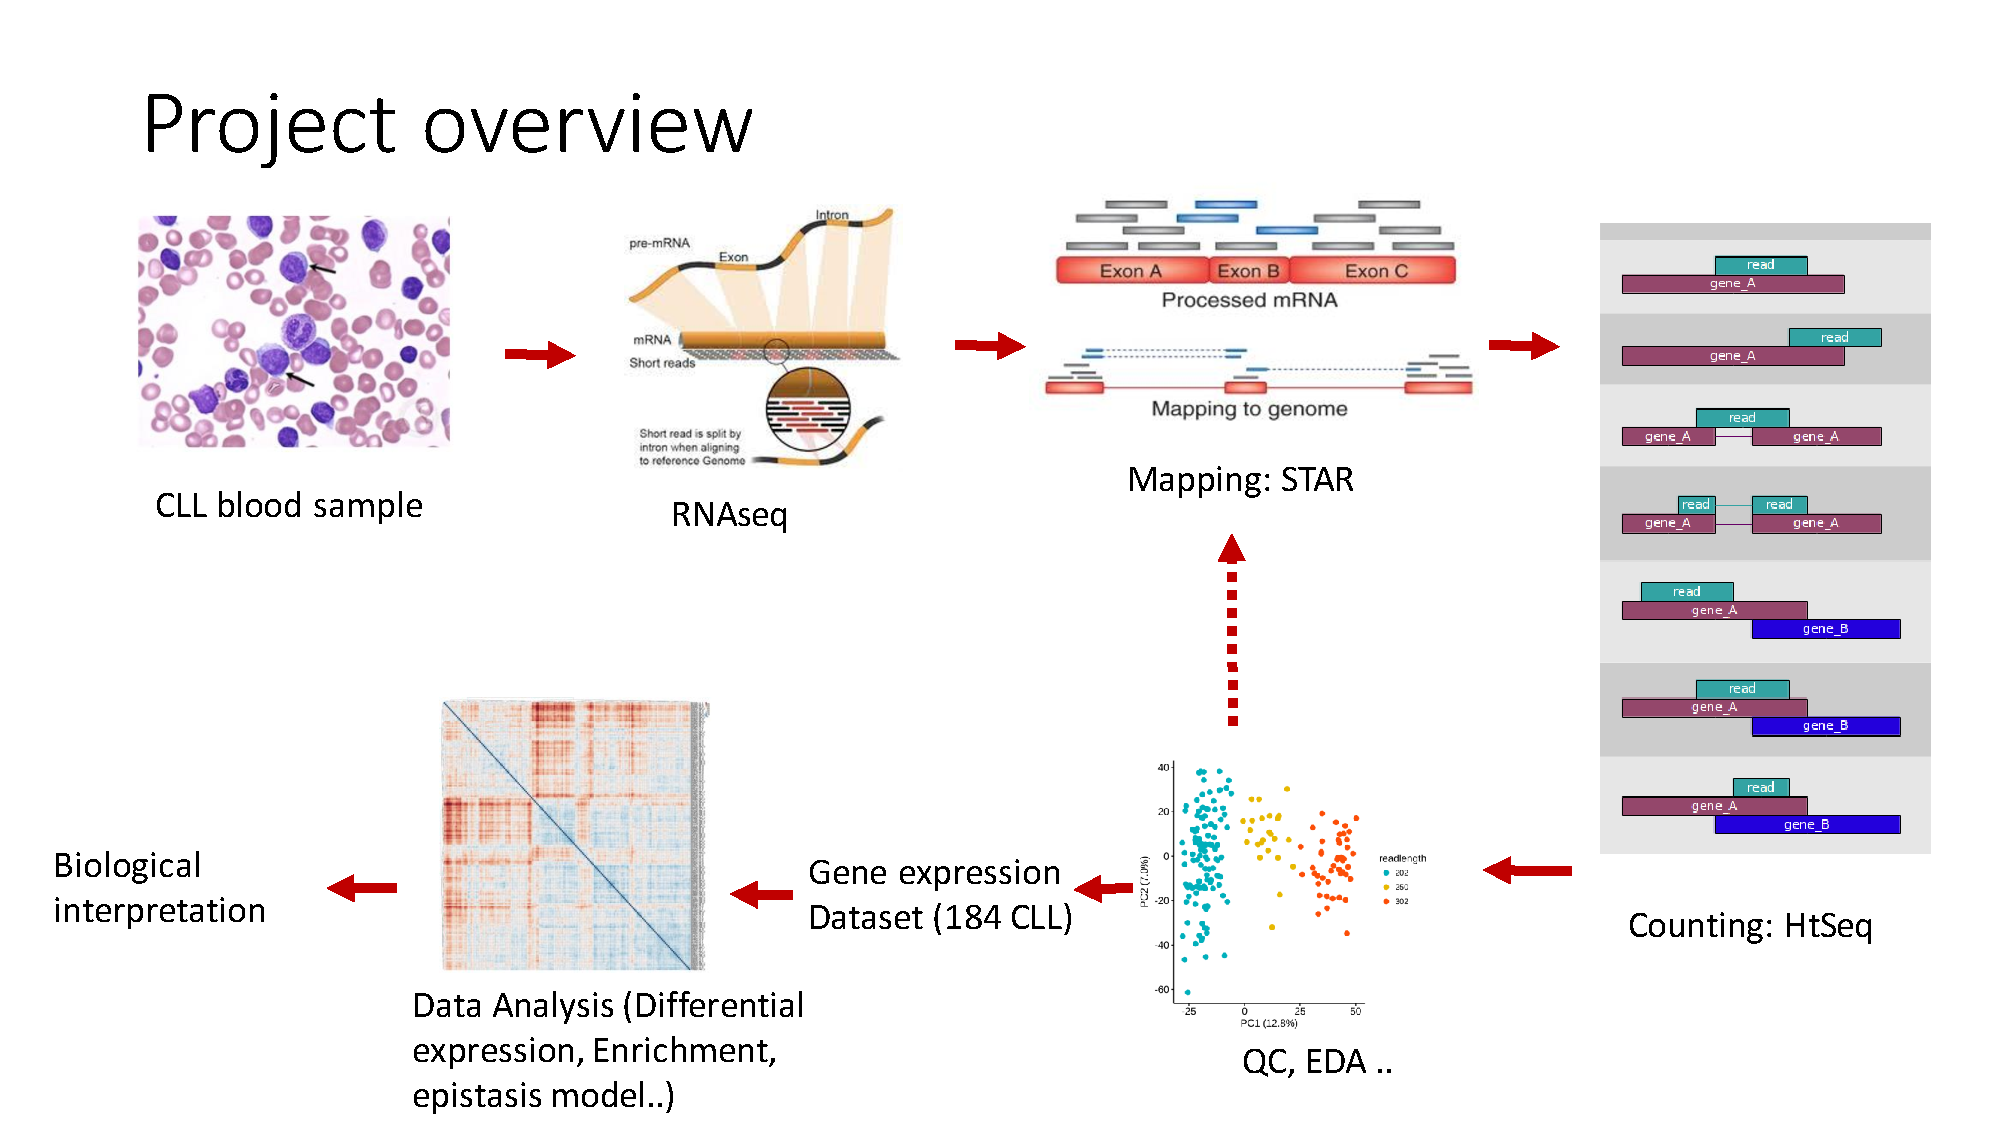
\includegraphics[width=\textwidth]{/home/almut/Dokumente/git/Transcriptome_CLL/presentation/figures/projectOverview.pdf}
%\caption{$x_V$: Victim's optimal SRM provision point. $x_I$: Injurer's optimal SRM provision point (Free-Driver Outcome).}
\end{figure}
\end{frame}
%
\section{Results}
%
%
\begin{frame}[c]
	\frametitle{Tumor epistasis - drug sensitivity}
	\begin{figure}
		\centering
		\begin{subfigure}[t]{0.48\columnwidth}
			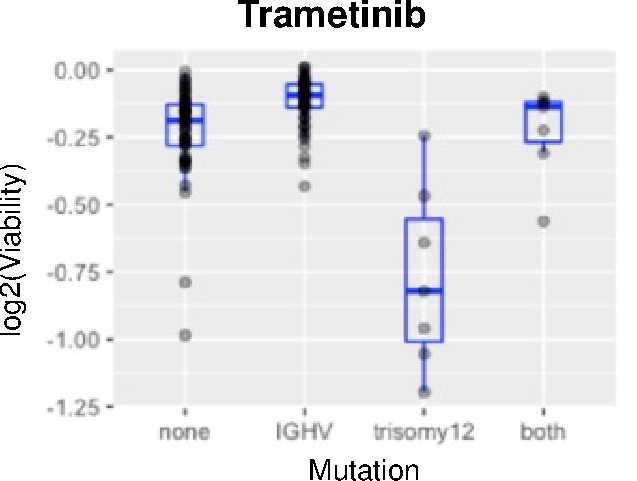
\includegraphics[width=\textwidth]{/home/almut/Dokumente/git/Transcriptome_CLL//presentation/figures/drugIII.pdf}
		\end{subfigure}
		\hfill
		\begin{subfigure}[t]{0.45\columnwidth}
			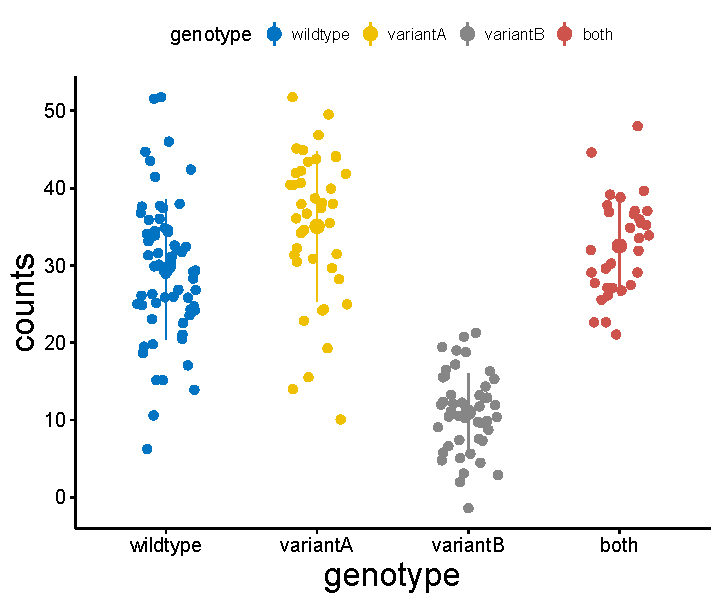
\includegraphics[width=\textwidth]{/home/almut/Dokumente/git/Transcriptome_CLL/thesis/Figures/genetic_interaction_concept.pdf}
		\end{subfigure}
	\end{figure}
	%\begin{itemize}
	%	\item \textbf{Trisomy12} sample are less/more sensitive in M-CLL
	%\end{itemize}
\end{frame}
%
%
\begin{frame}[c]
	\frametitle{Epistatic interaction of Trisomy12 and IGHV}
	\begin{figure}
		\centering
		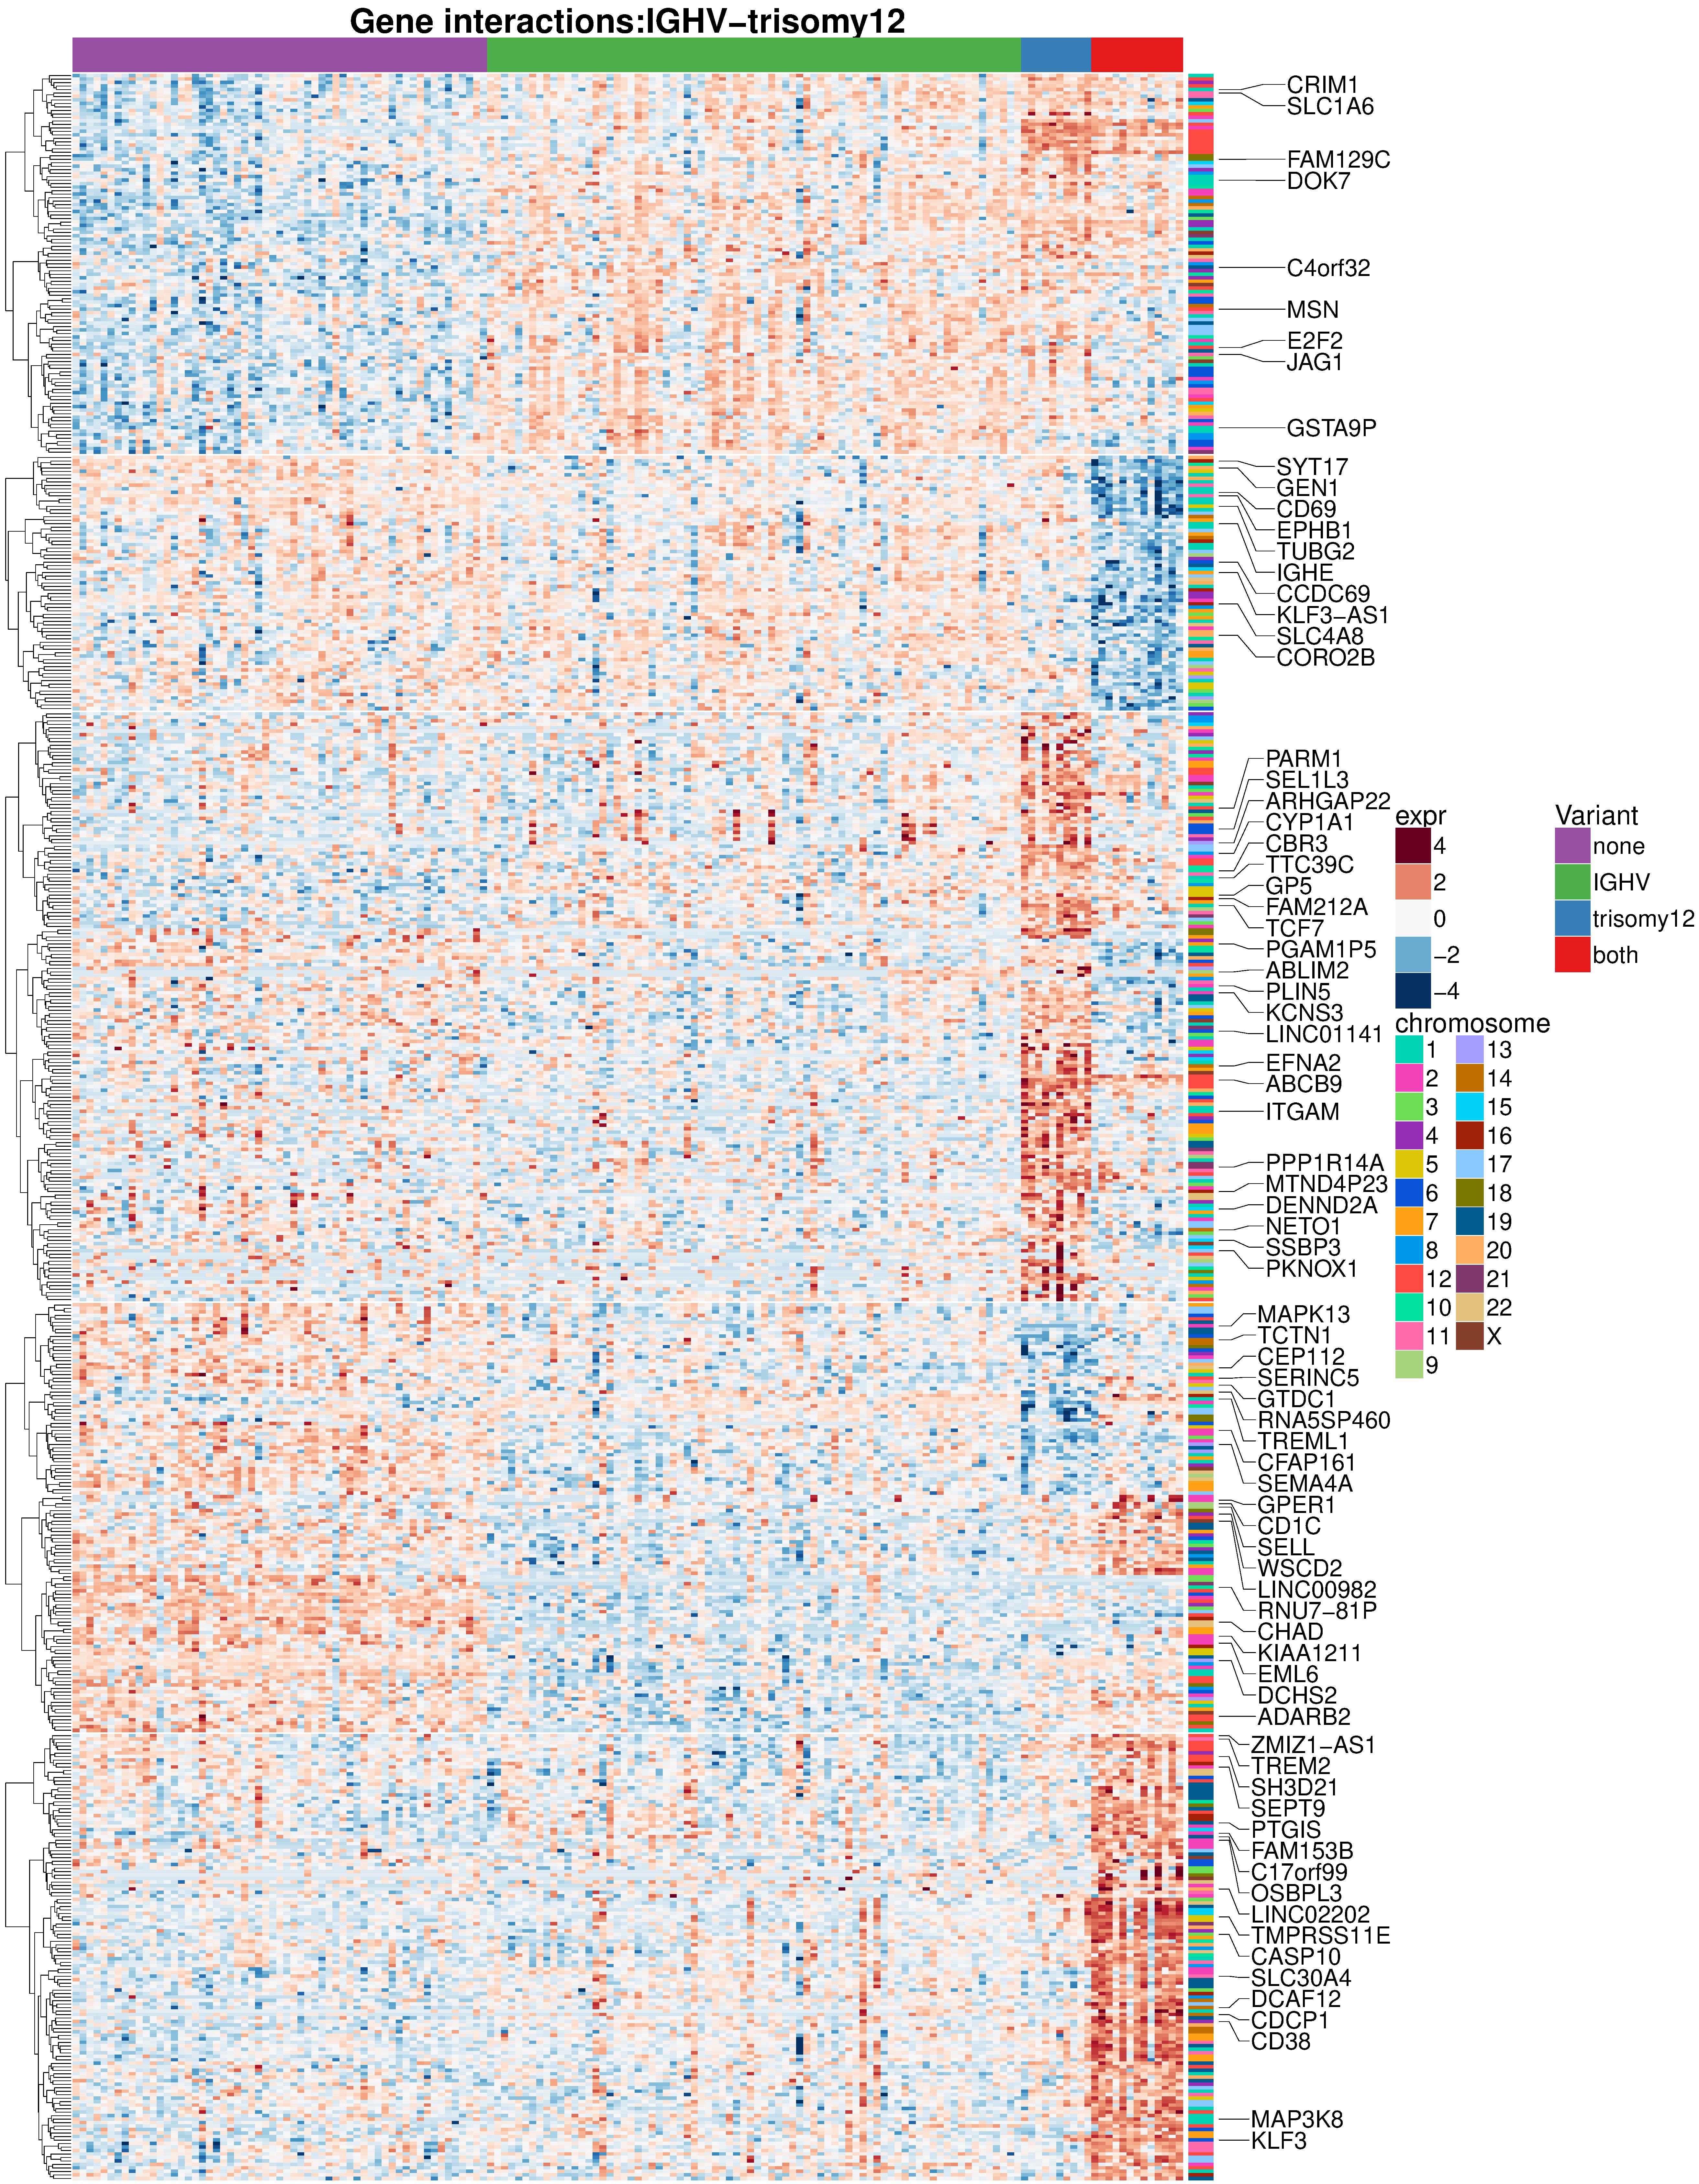
\includegraphics[width=0.5\textwidth]{/home/almut/Dokumente/git/Transcriptome_CLL/thesis/Figures/epistatsisTri12IGHV_withoutDirs.pdf}
	\end{figure}
\end{frame}

% 
%%% Backup slides %%%%%%%%%%%%%%%%%%%%%%%%%%%%%%%%%%%%%%%%%%%%%%%%%%%%%%%%%%%%%%%%%%%%%%%%%%%%%%%%%%%%%%%%
% Note that these slides are not taken into account when computing the total number of slides of the presentation.

\appendix
\section{Appendix}
%
%
%
\begin{frame}[c]
	\frametitle{Thanks to ..}
	\begin{figure}
		\centering
		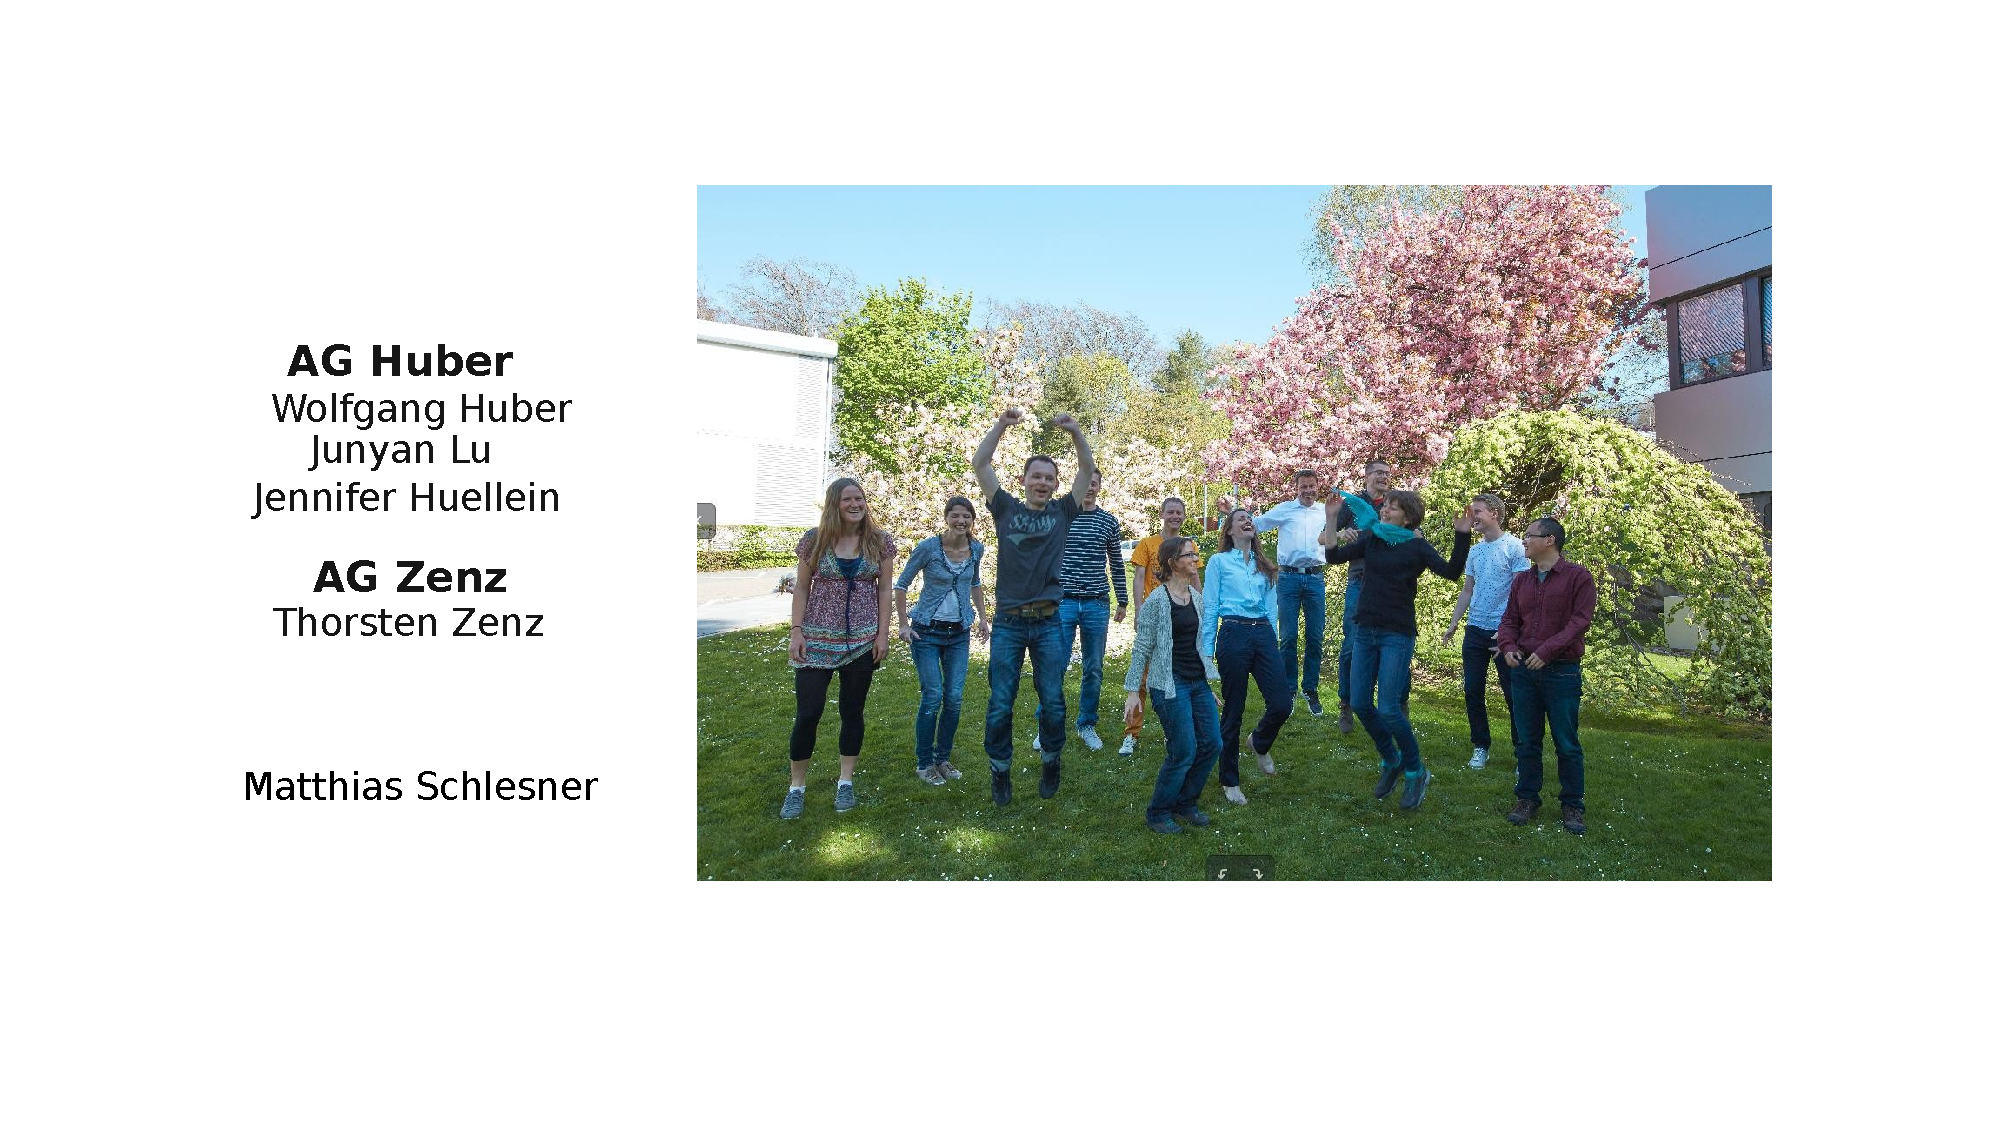
\includegraphics[width=\textwidth]{/home/almut/Dokumente/git/Transcriptome_CLL/presentation/figures/group.pdf}
	\end{figure}
\end{frame}
%
\section{models}
%
%
%
\section{Gene expression signatures}
%
%
\begin{frame}[c]
	\frametitle{Mixed epistasis model}
	\begin{figure}
		\centering
		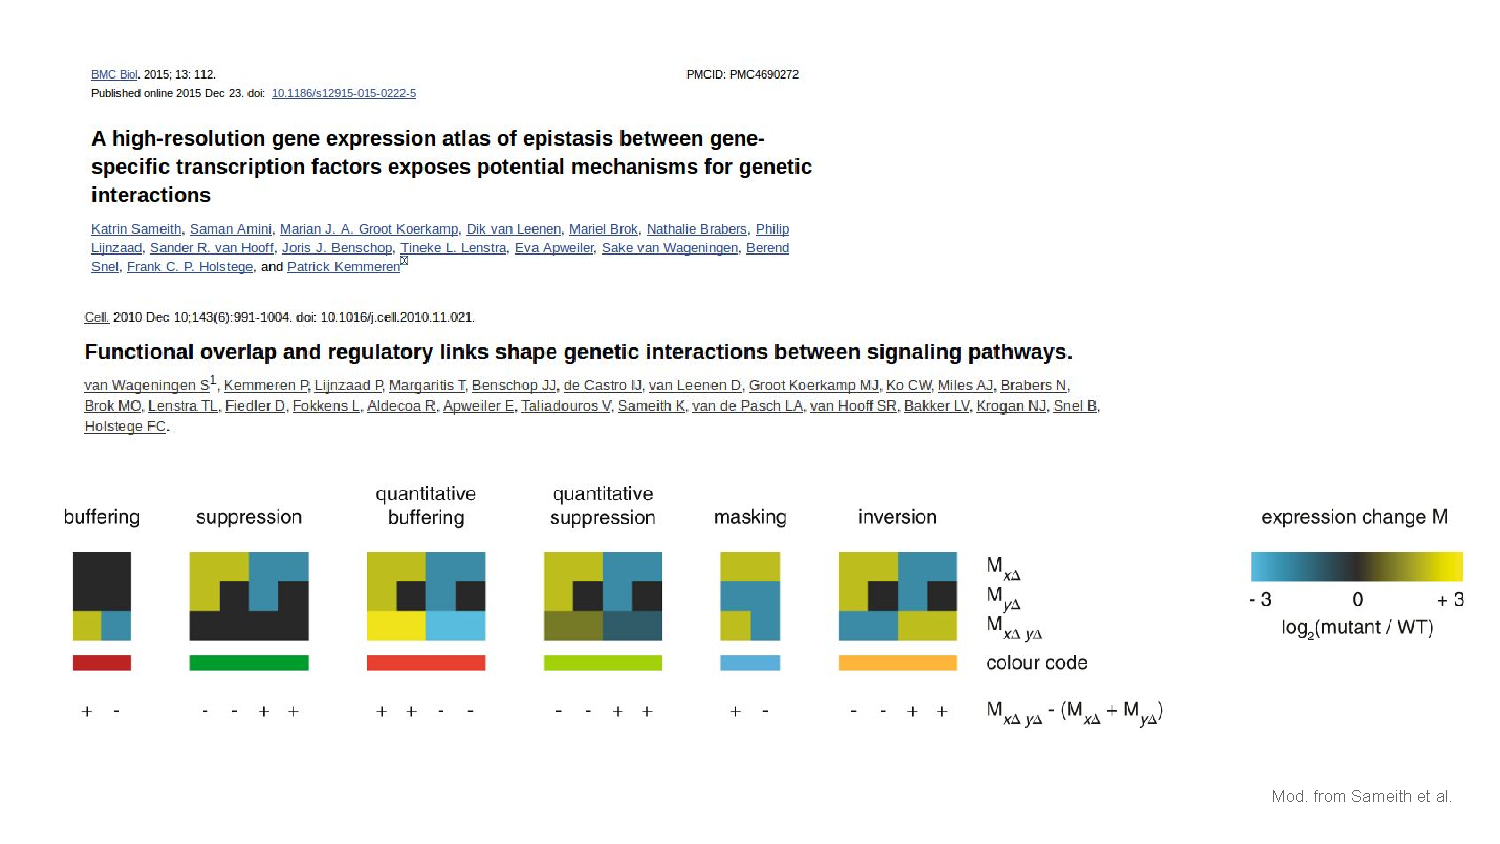
\includegraphics[width=\textwidth]{/home/almut/Dokumente/git/Transcriptome_CLL/presentation/figures/Mixed_epistasis_model.pdf}
	\end{figure}
\end{frame}
%
%
\begin{frame}[c]
	\frametitle{Hierachical Clustering}
	\begin{figure}
		\centering
		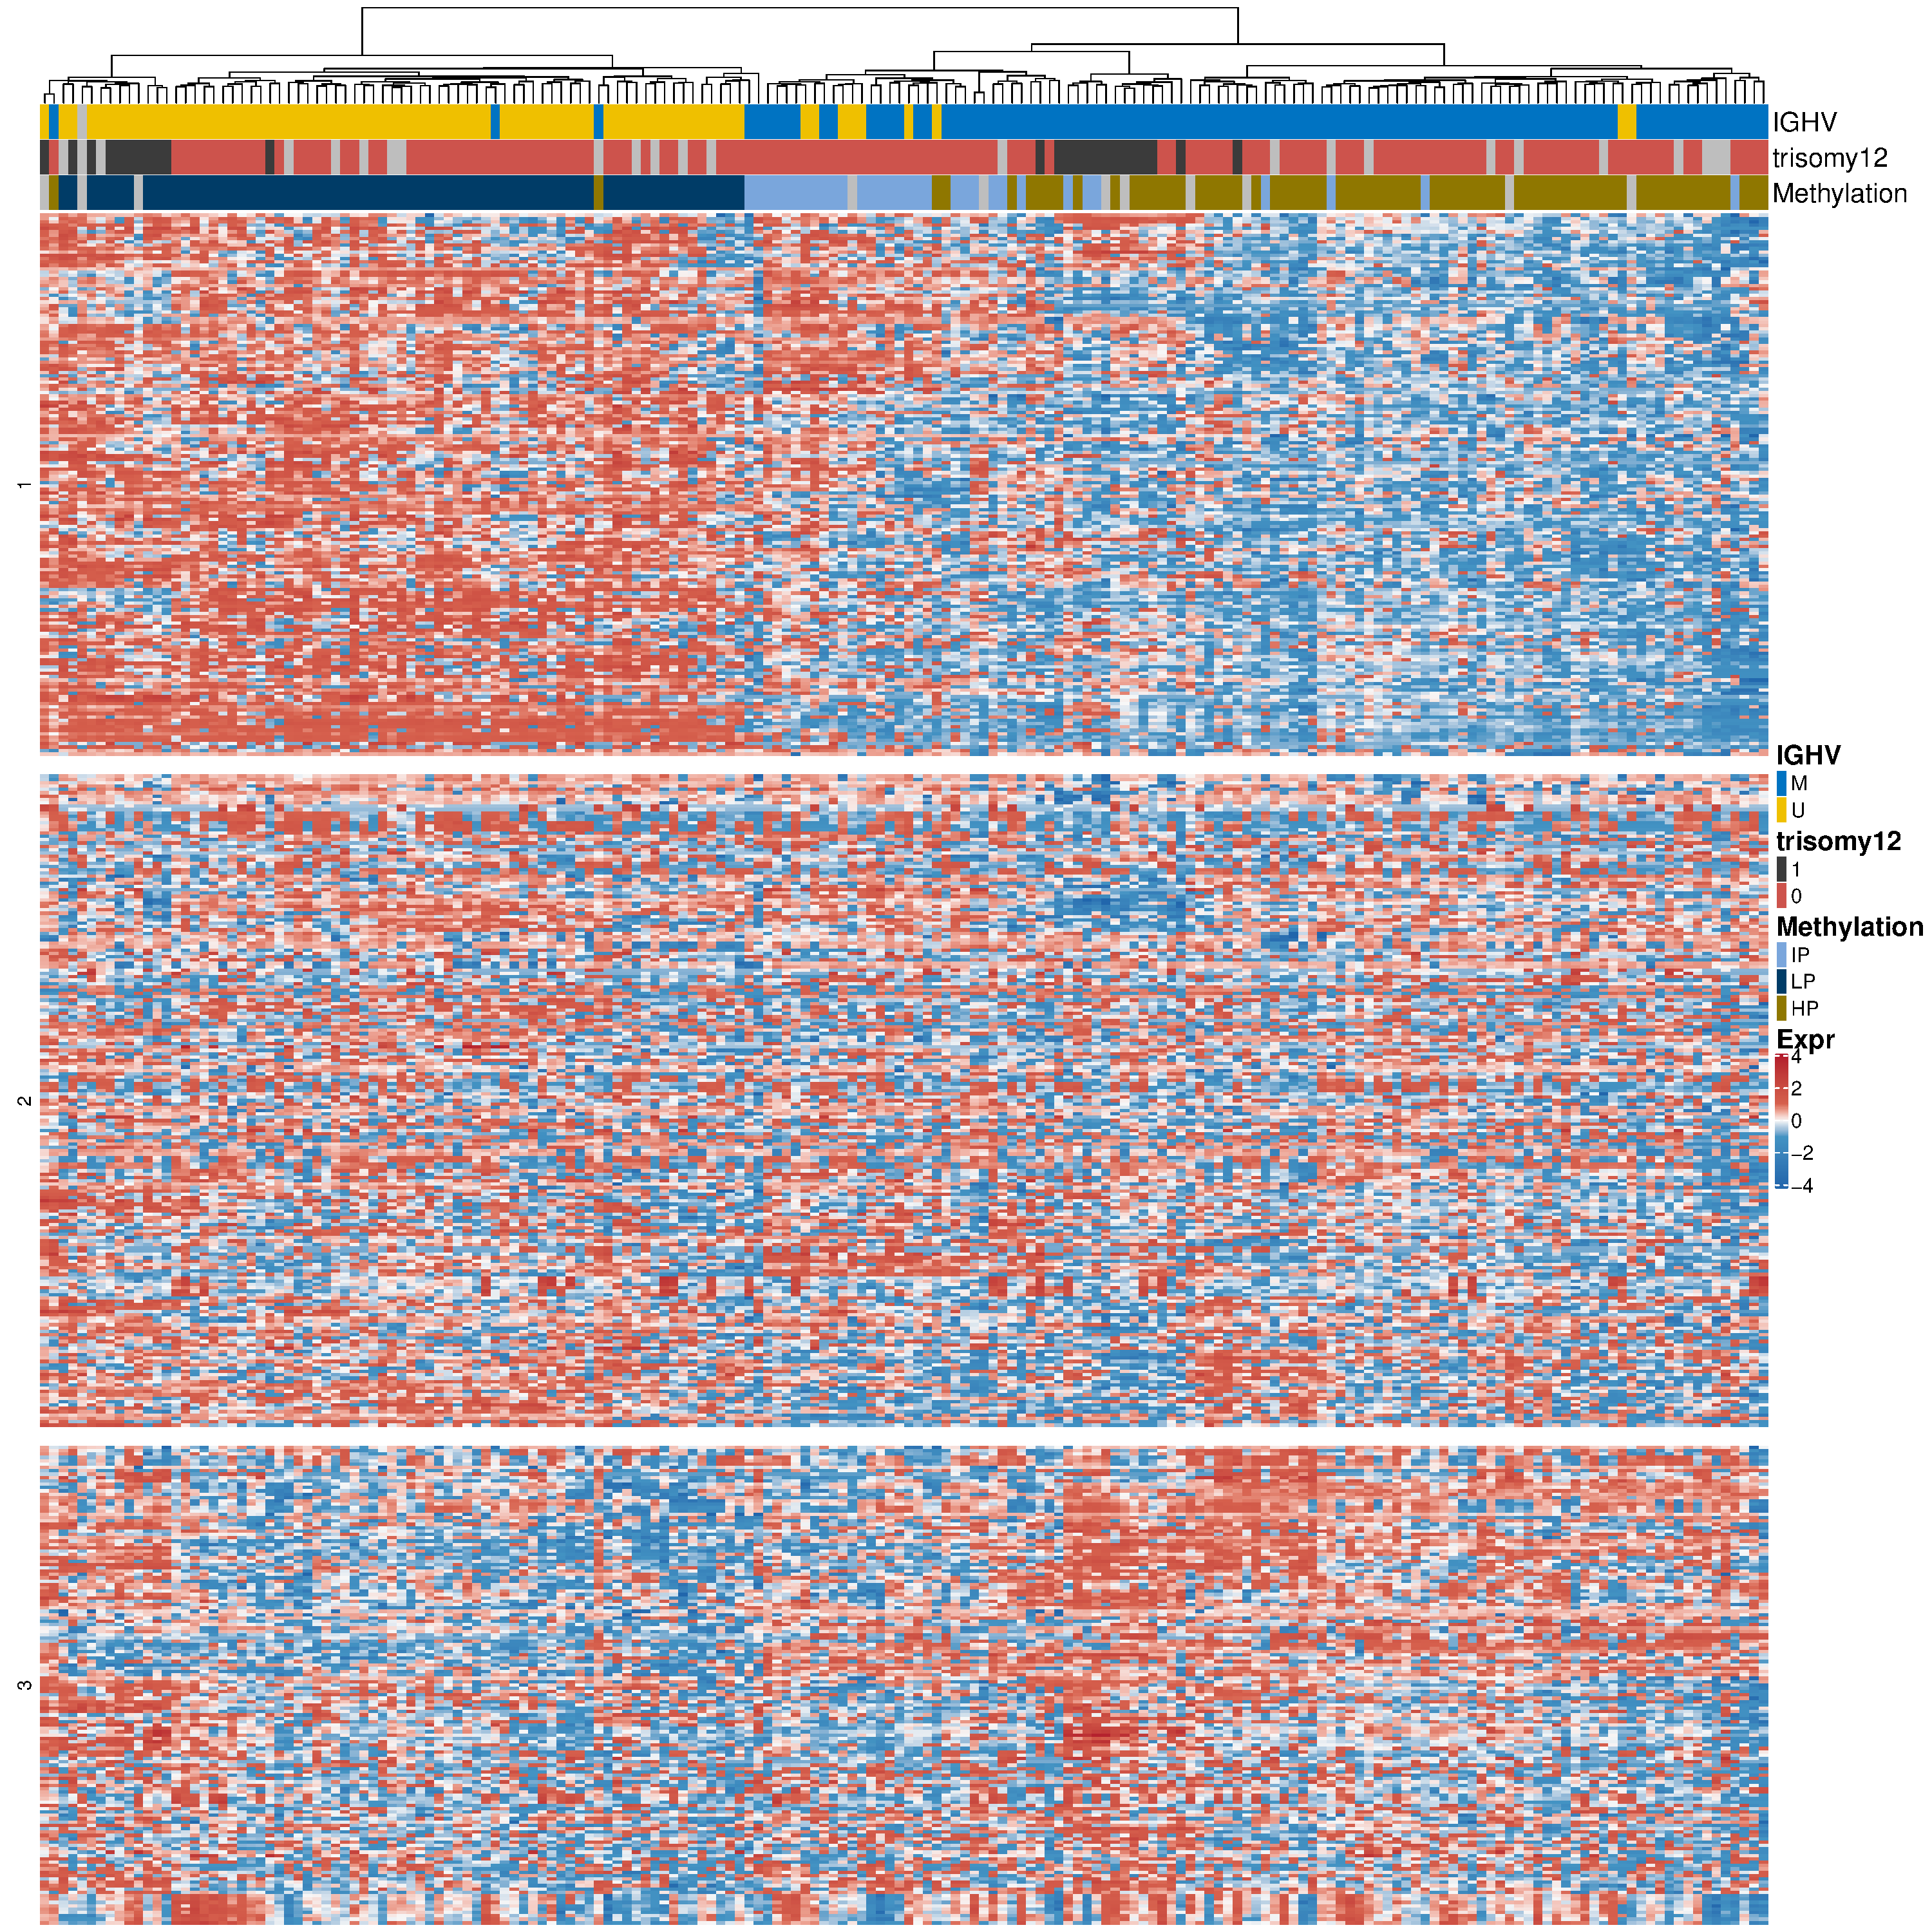
\includegraphics[width=0.7\textwidth]{/home/almut/Dokumente/git/Transcriptome_CLL/thesis/Figures/cluster500exprgenes.pdf}
	\end{figure}
\end{frame}
%
%
\begin{frame}[c]
	\frametitle{Trisomy12 signature}
	\begin{figure}
		\centering
		\includegraphics[width=0.7\textwidth]{/home/almut/Dokumente/git/Transcriptome_CLL/thesis/Figures/gene_exprTrisomy12_gsea_Hallmark.pdf}
	\end{figure}
\end{frame}
% 
\begin{frame}[c]
	\frametitle{Multivariate model}
	\begin{minipage}[t]{.67\textwidth}
		\begin{figure}
			%\centering
			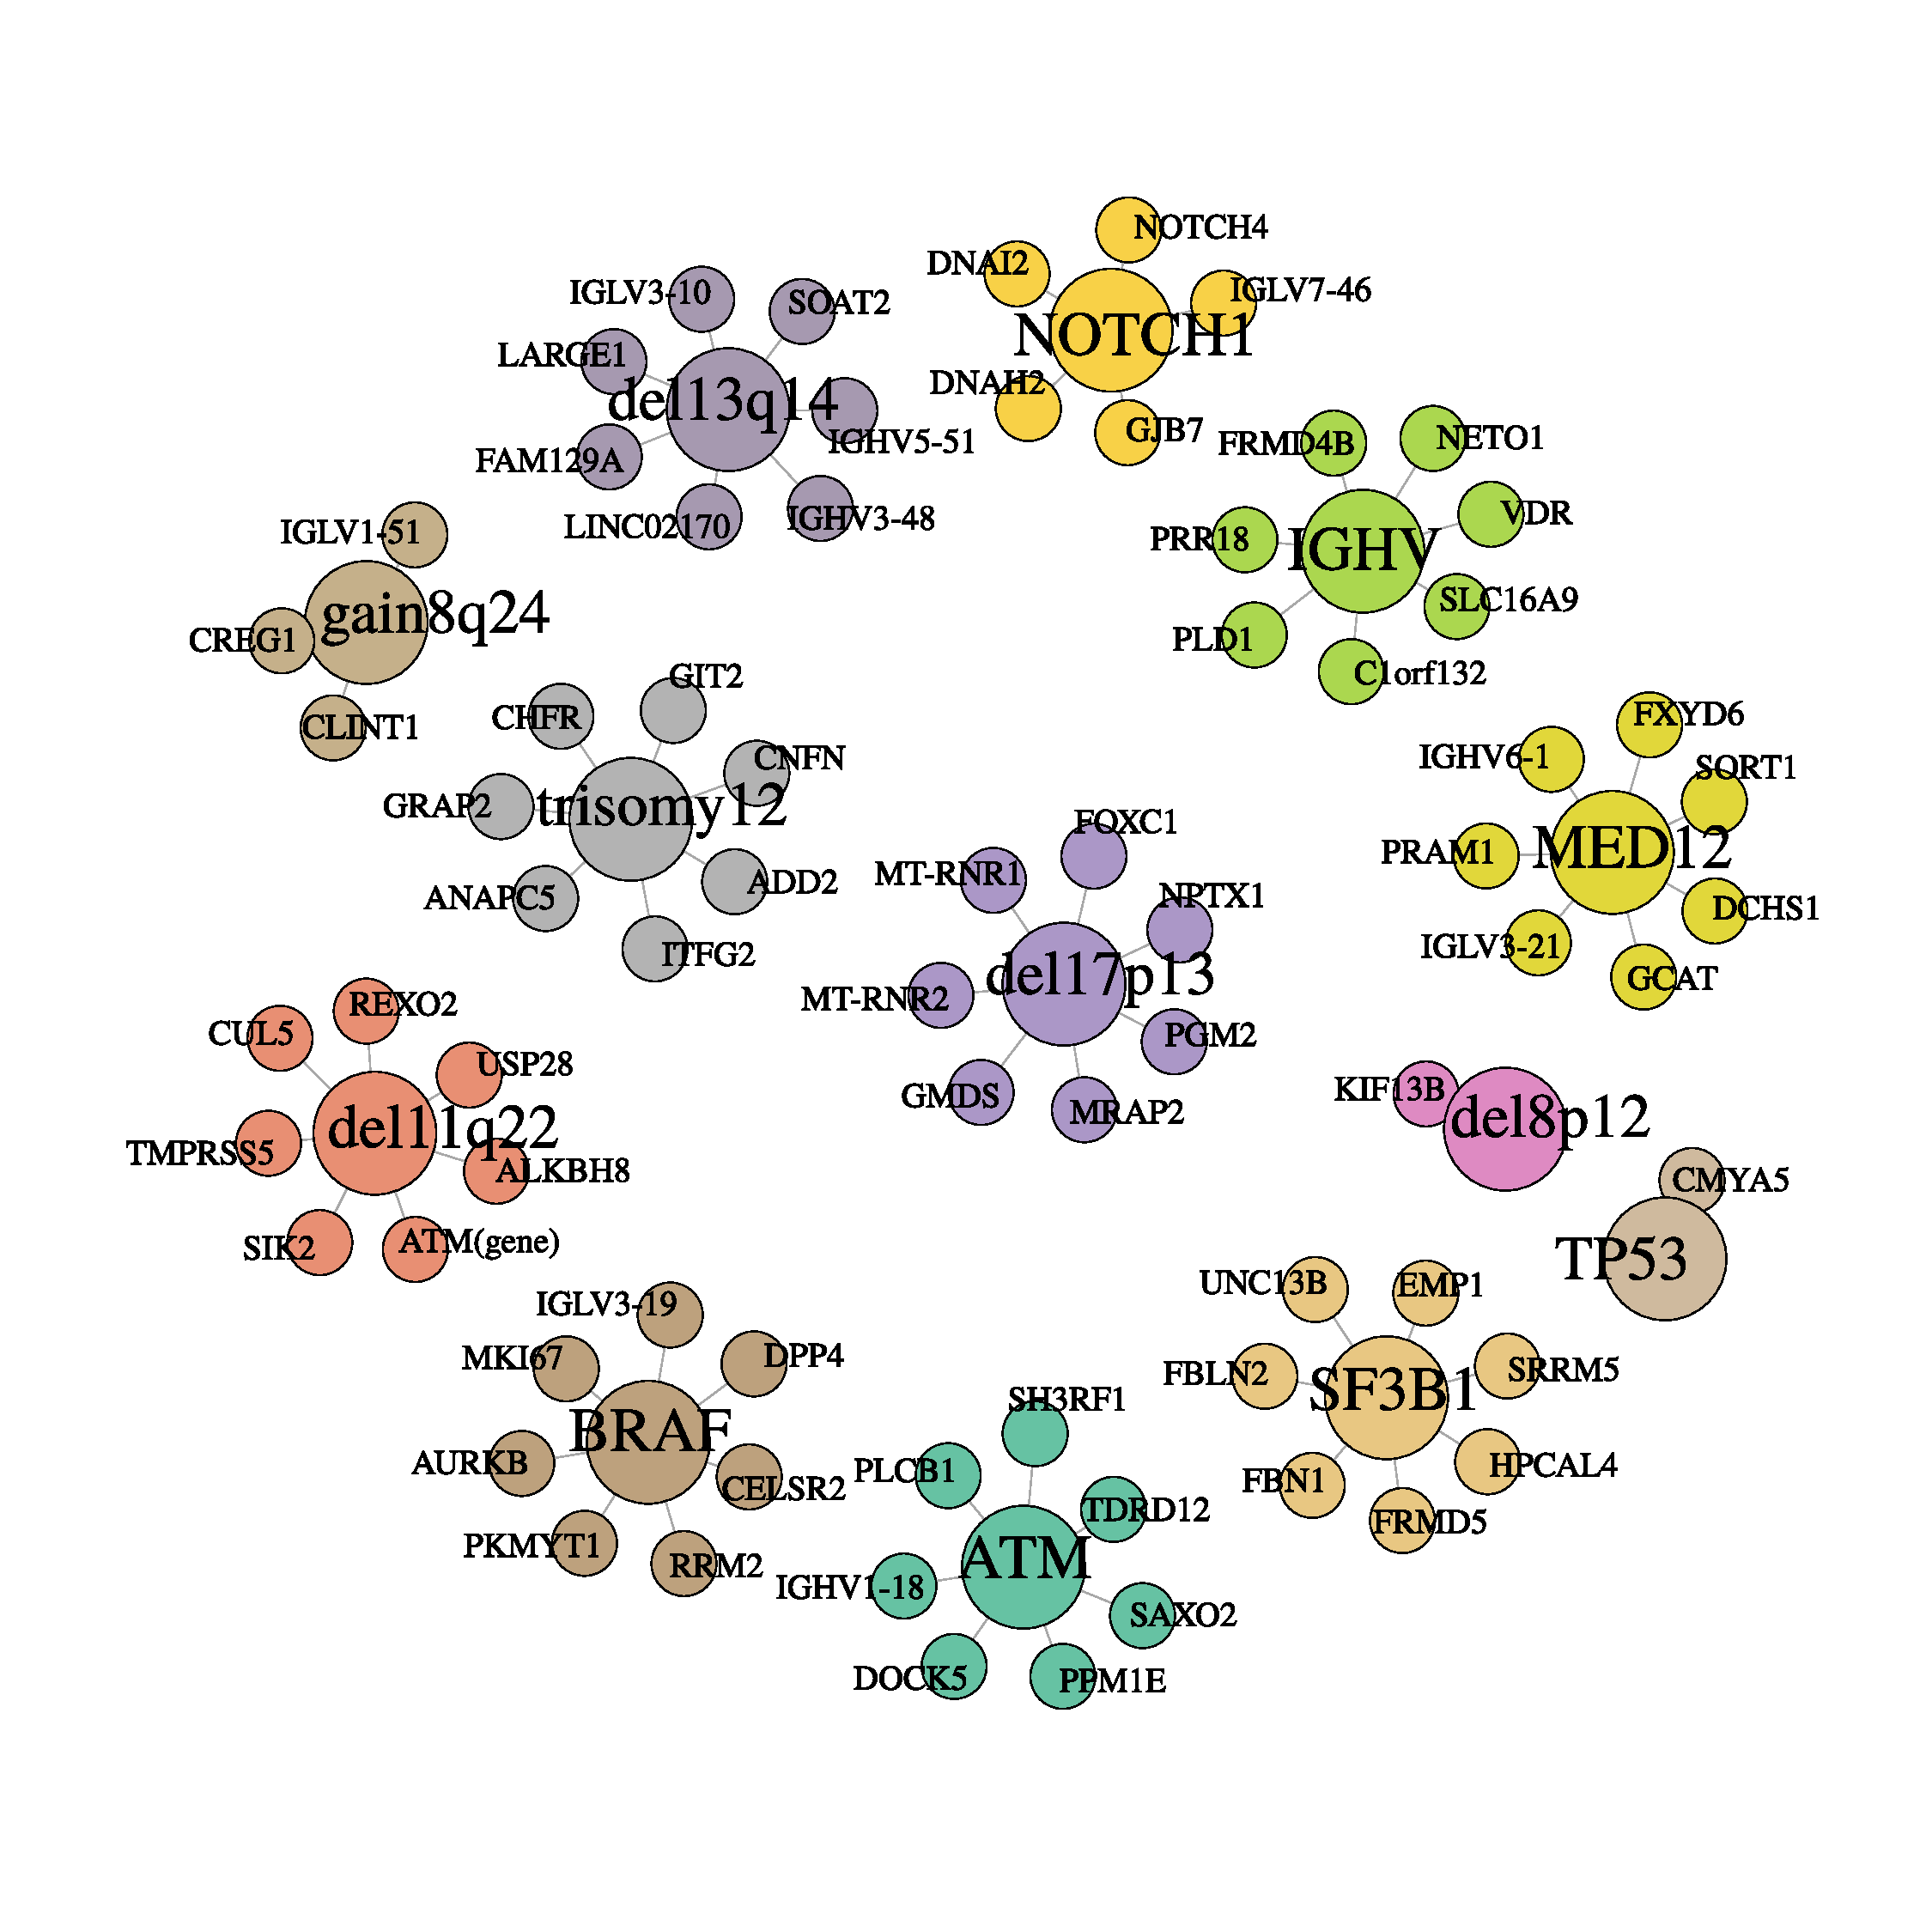
\includegraphics[width=\columnwidth]{/home/almut/Dokumente/git/Transcriptome_CLL/thesis/Figures/reducedModel.pdf}
		\end{figure}
	\end{minipage}
	\begin{minipage}[t]{.3\textwidth}
		\begin{itemize}
			\item Individual effect of each variant
			\item Likelihood ratio test of complete and reduced model
		\end{itemize}
	\end{minipage}
\end{frame}
% 
%
\begin{frame}[c]
	\frametitle{Tumor epistasis - genetic interaction}
	\begin{figure}
		\centering
		%\begin{subfigure}[t]{0.65\columnwidth}
		%	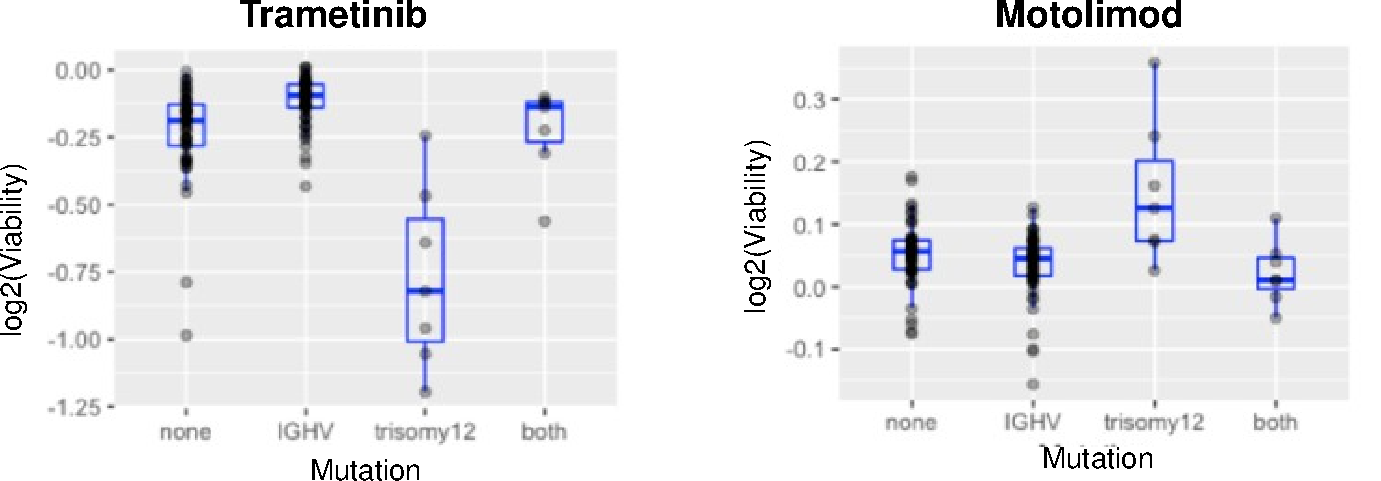
\includegraphics[width=\textwidth]{/home/almut/Dokumente/git/Transcriptome_CLL//presentation/figures/drugII.pdf}
		%\end{subfigure}
		%\hfill
		\begin{subfigure}[t]{0.45\columnwidth}
			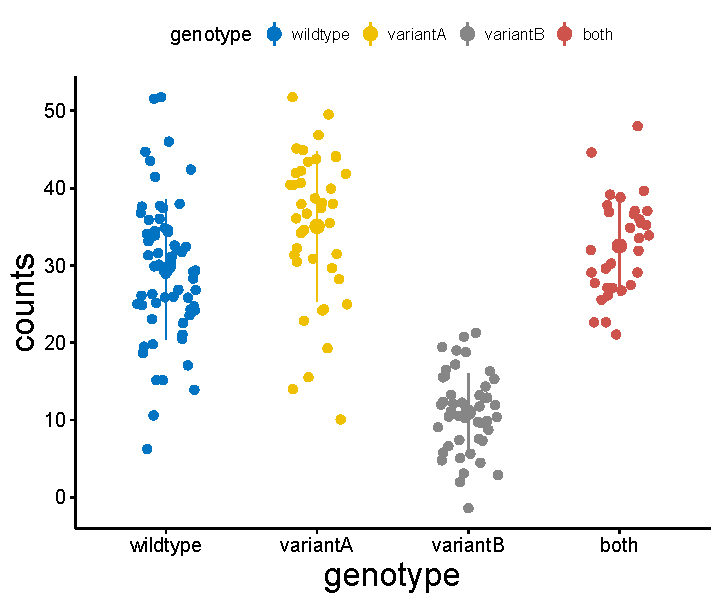
\includegraphics[width=\textwidth]{/home/almut/Dokumente/git/Transcriptome_CLL/thesis/Figures/genetic_interaction_concept.pdf}
		\end{subfigure}
	\end{figure}
	\begin{itemize}
		\item Observed gene expression in a combined genotype differs from the expected expression by combination of the individual effects
	\end{itemize}
\end{frame}
%
\begin{frame}[c]
	\frametitle{Genomic variants}
	\begin{figure}
		\centering
		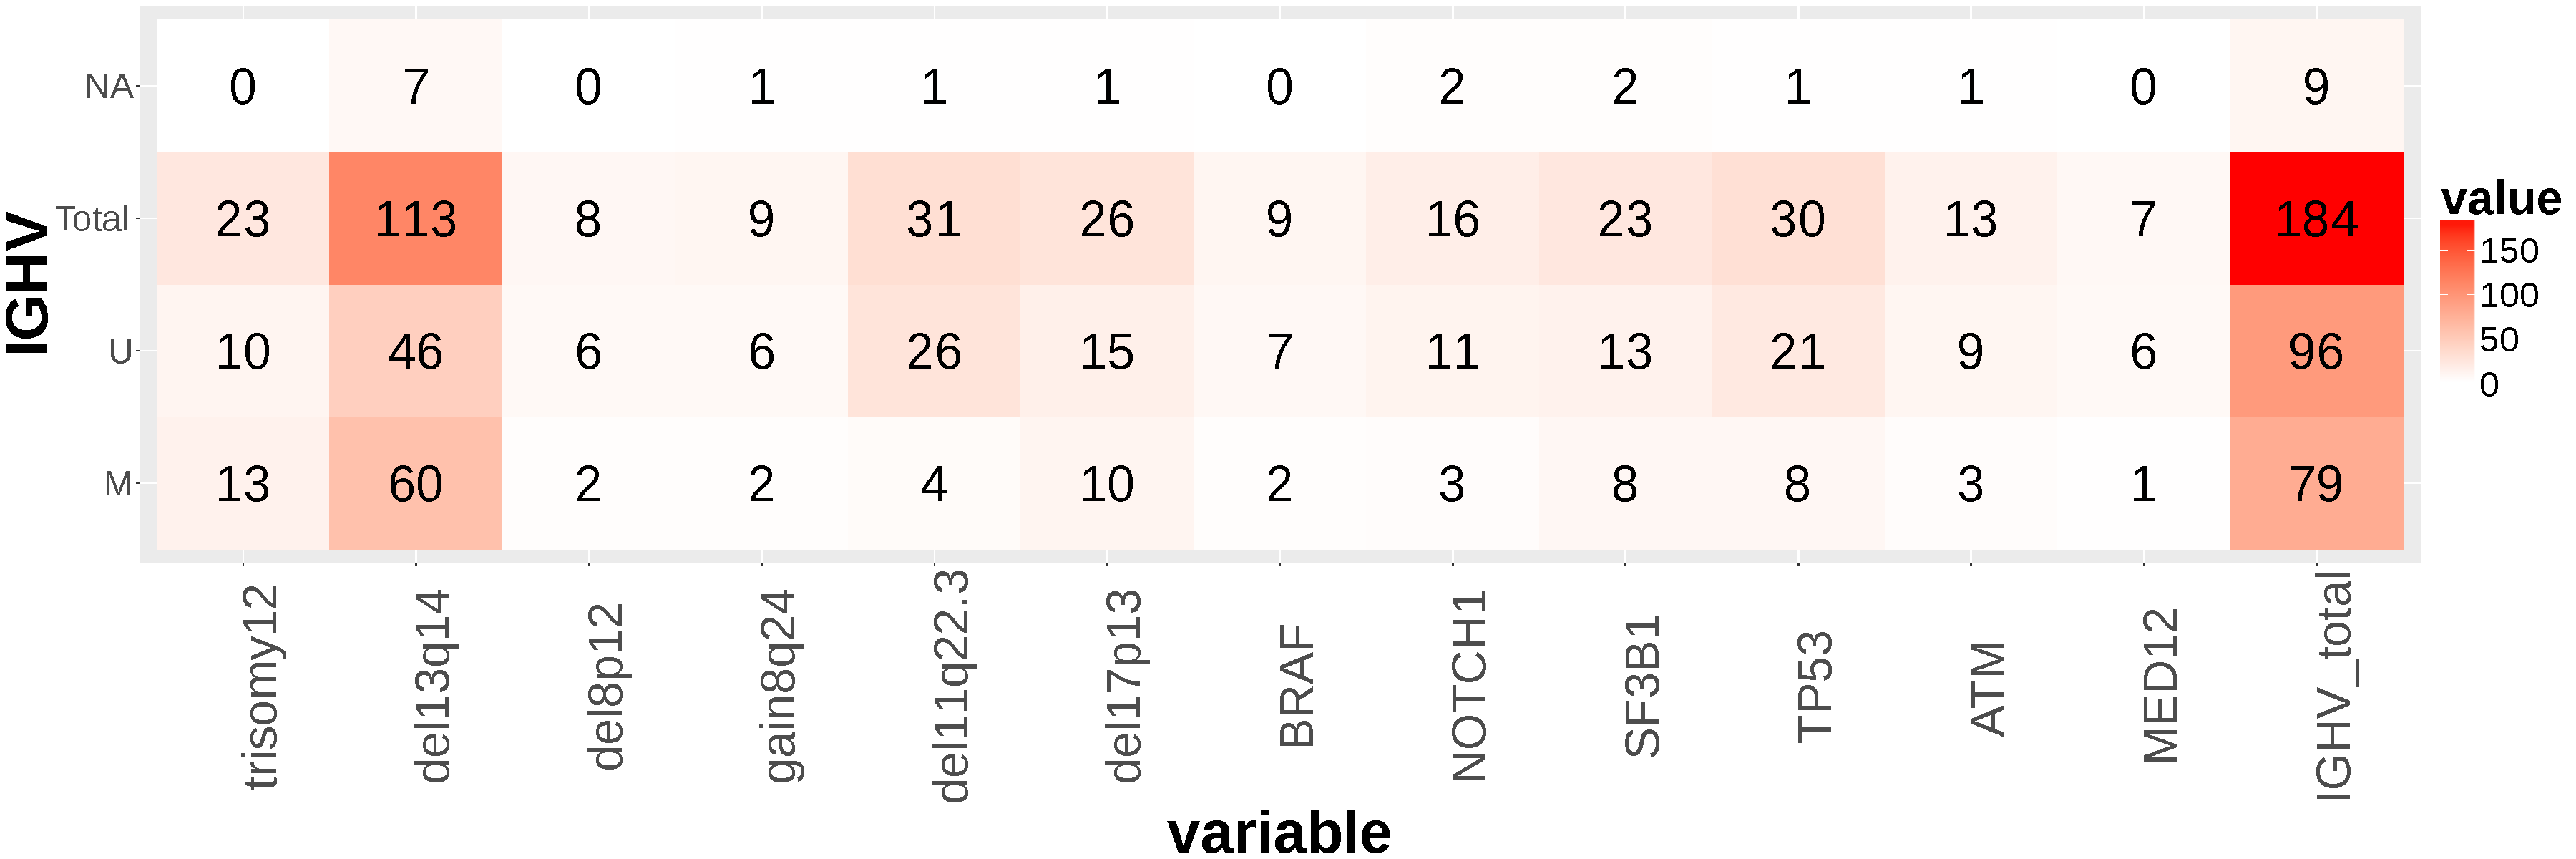
\includegraphics[width=\textwidth]{/home/almut/Dokumente/git/Transcriptome_CLL/thesis/Figures/datatable_overview.pdf}
	\end{figure}
\end{frame}
%
%
\begin{frame}[c]
	\frametitle{Principal Component Analysis}
	\begin{figure}
		\centering
		\begin{subfigure}[t]{0.45\columnwidth}
			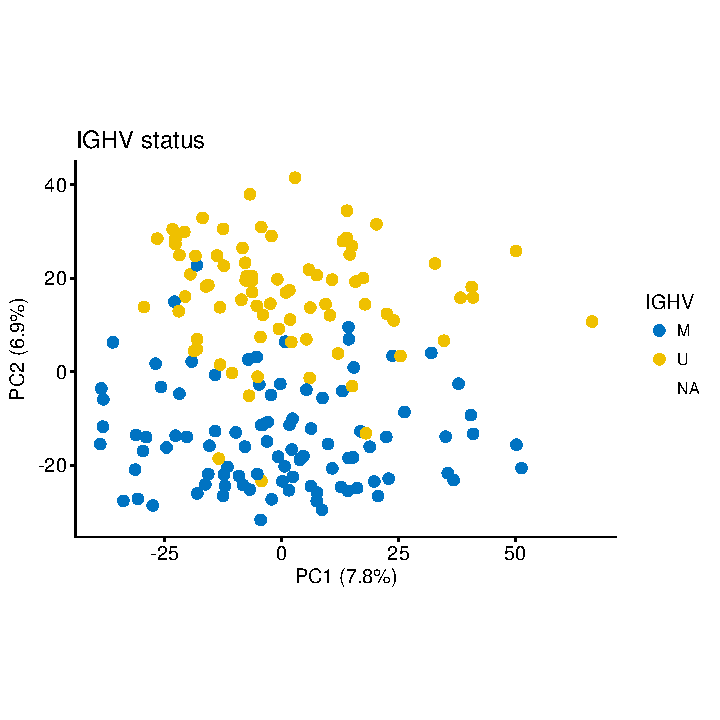
\includegraphics[width=\textwidth]{/home/almut/Dokumente/git/Transcriptome_CLL/presentation/figures/pca_ighv.pdf}
		\end{subfigure}
		\hfill
		\begin{subfigure}[t]{0.45\columnwidth}
			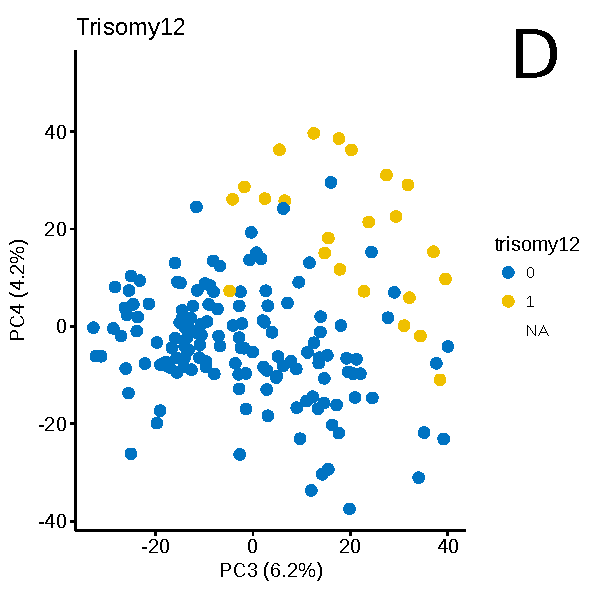
\includegraphics[width=\textwidth]{/home/almut/Dokumente/git/Transcriptome_CLL/presentation/figures/pca_trisomy12.pdf}
		\end{subfigure}
	\end{figure}
\end{frame}
% 
%
\begin{frame}[c]
	\frametitle{IGHV signature}
	\begin{figure}
		\centering
		\includegraphics[width=0.7\textwidth]{/home/almut/Dokumente/git/Transcriptome_CLL/thesis/Figures/gene_exprIGHV_gsea_Hallmark.pdf}
	\end{figure}
\end{frame}
%
%
\begin{frame}[c]
	\frametitle{Trisomy12 signature}
	\begin{figure}
		\centering
		\begin{subfigure}[t]{0.45\columnwidth}
			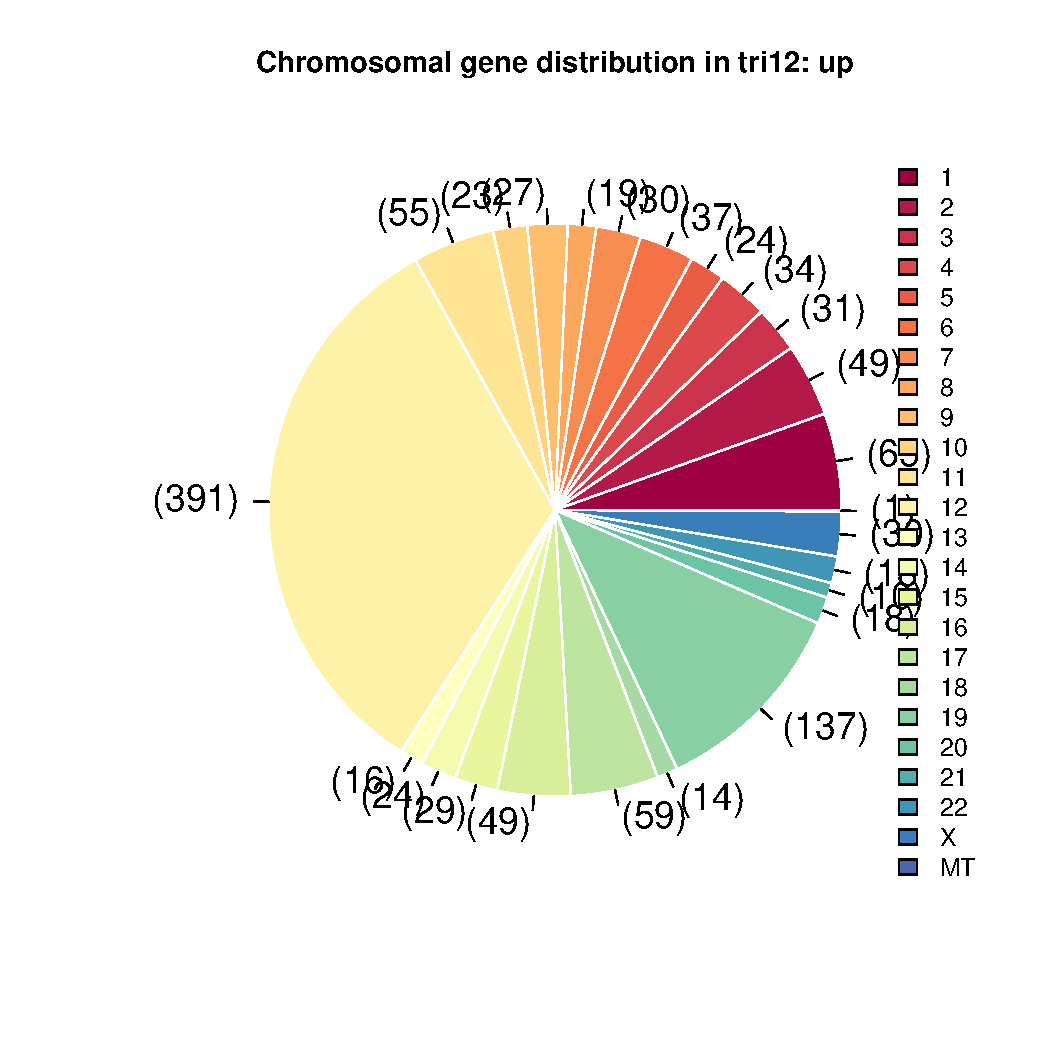
\includegraphics[width=\textwidth]{/home/almut/Dokumente/git/Transcriptome_CLL/presentation/figures/chromosom_dist_up.pdf}
		\end{subfigure}
		\hfill
		\begin{subfigure}[t]{0.45\columnwidth}
			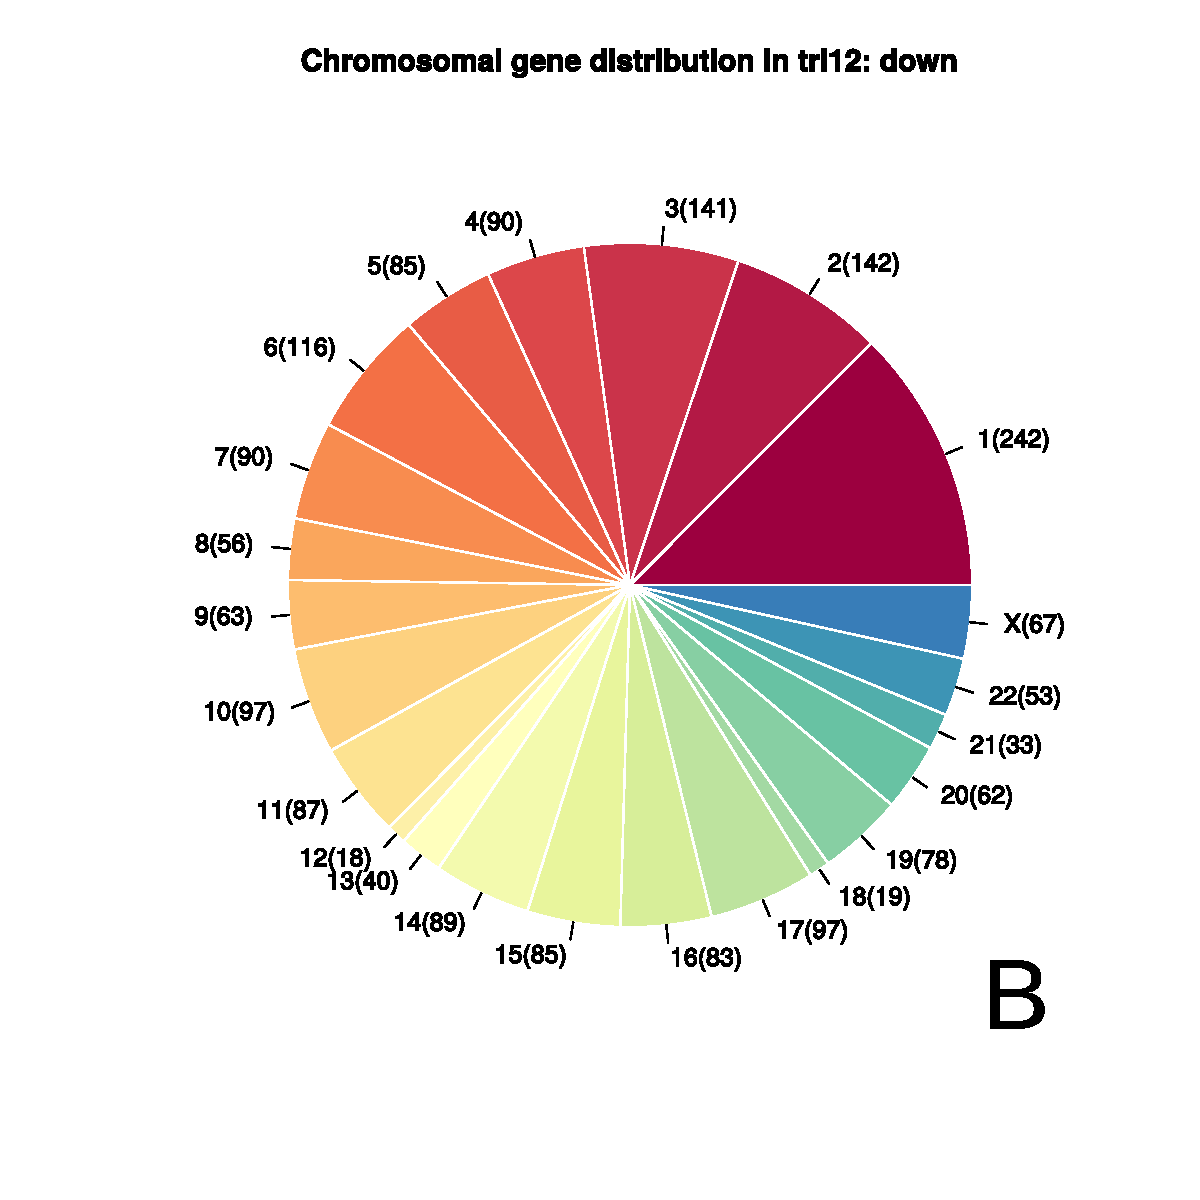
\includegraphics[width=\textwidth]{/home/almut/Dokumente/git/Transcriptome_CLL/presentation/figures/chromosom_dist_down.pdf}
		\end{subfigure}
	\end{figure}
\end{frame}
%
\begin{frame}[c]
	\frametitle{Summary I}	
	\begin{itemize}
		\item Most comprehensive CLL transcriptome dataset (Primary blood cancer cell encyclopedia)
		\item \textbf{IGHV} status and \textbf{Trisomy12} have major impact on gene expression
		\begin{itemize}
			\item 6.9\% variance are associated to IGHV, compared to 1.5\% in previous studies (Feirrera et al. 2014)
		\end{itemize}
		\item Associations between variants (e.g. Del11q22/IGHV, Del17p13/TP53, ..)
	\end{itemize}
\end{frame}
%
%
\begin{frame}[c]
\frametitle{T cell contamination}
		\begin{figure}
			\centering
			\begin{subfigure}[t]{0.5\columnwidth}
				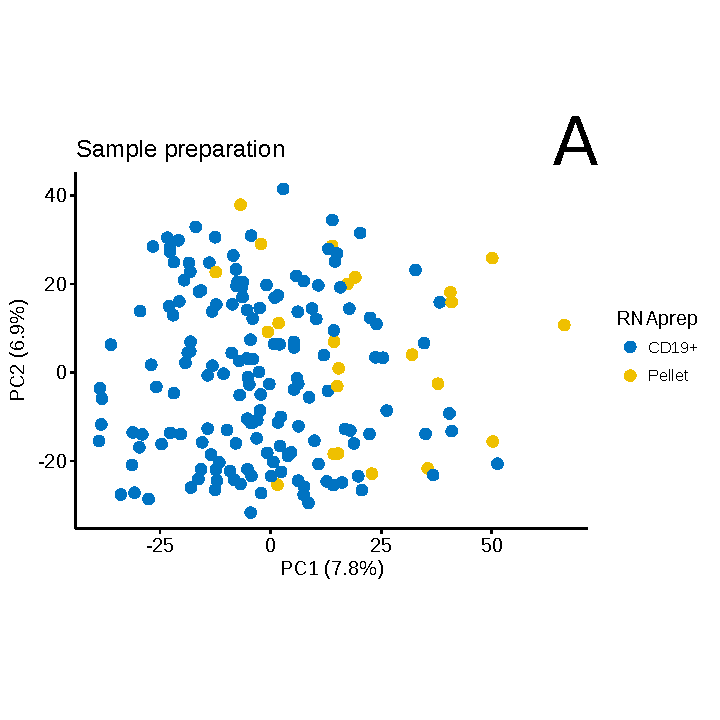
\includegraphics[width=\textwidth]{/home/almut/Dokumente/git/Transcriptome_CLL/presentation/figures/pca_RNAprep.pdf}
			\end{subfigure}
			\hfill
			\begin{subfigure}[t]{0.5\columnwidth}
				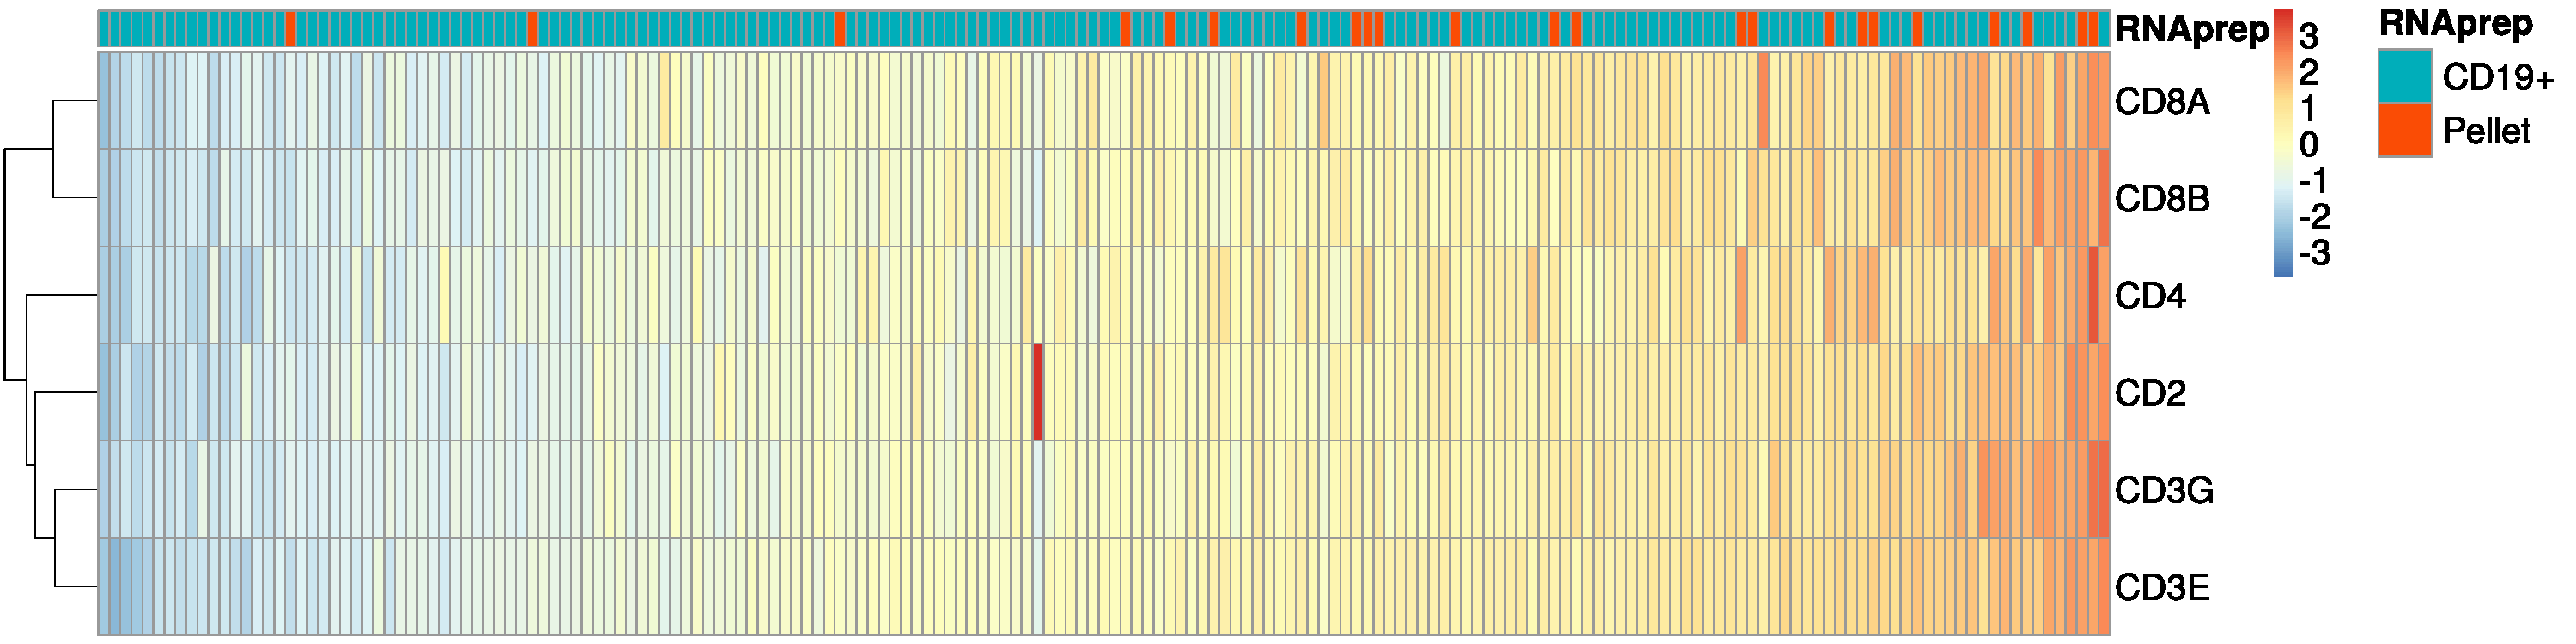
\includegraphics[width=\textwidth]{/home/almut/Dokumente/git/Transcriptome_CLL/presentation/figures/TmarkExpression.pdf}
			\end{subfigure}
		\end{figure}
\end{frame}
%
%
\begin{frame}[c]
	\frametitle{Adapter contamination}
	\begin{figure}
		\centering
		\begin{subfigure}[t]{0.48\columnwidth}
			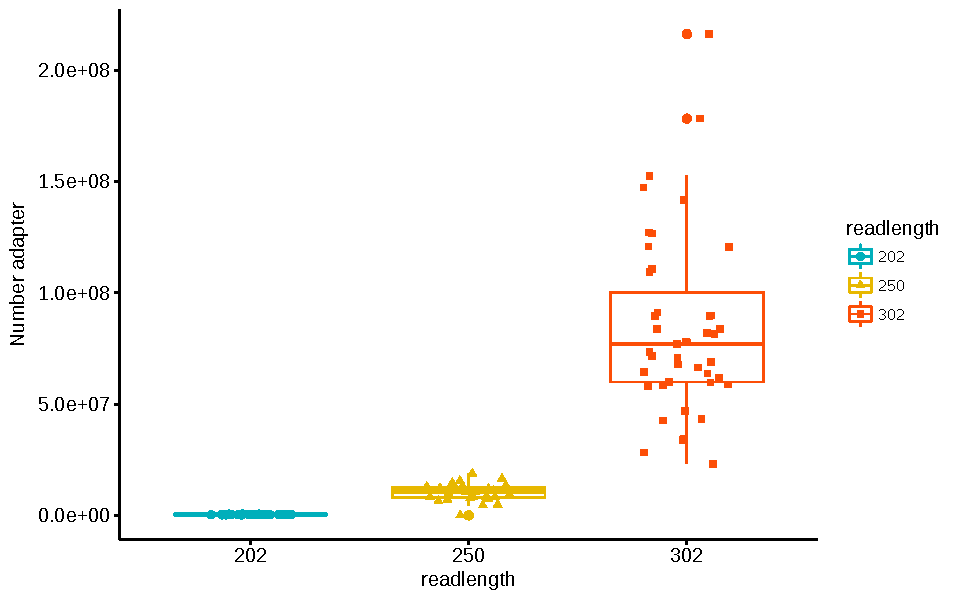
\includegraphics[width=\textwidth]{/home/almut/Dokumente/git/Transcriptome_CLL/thesis/Figures/adapter_contam.pdf}
		\end{subfigure}
		\hfill
		\begin{subfigure}[t]{0.43\columnwidth}
			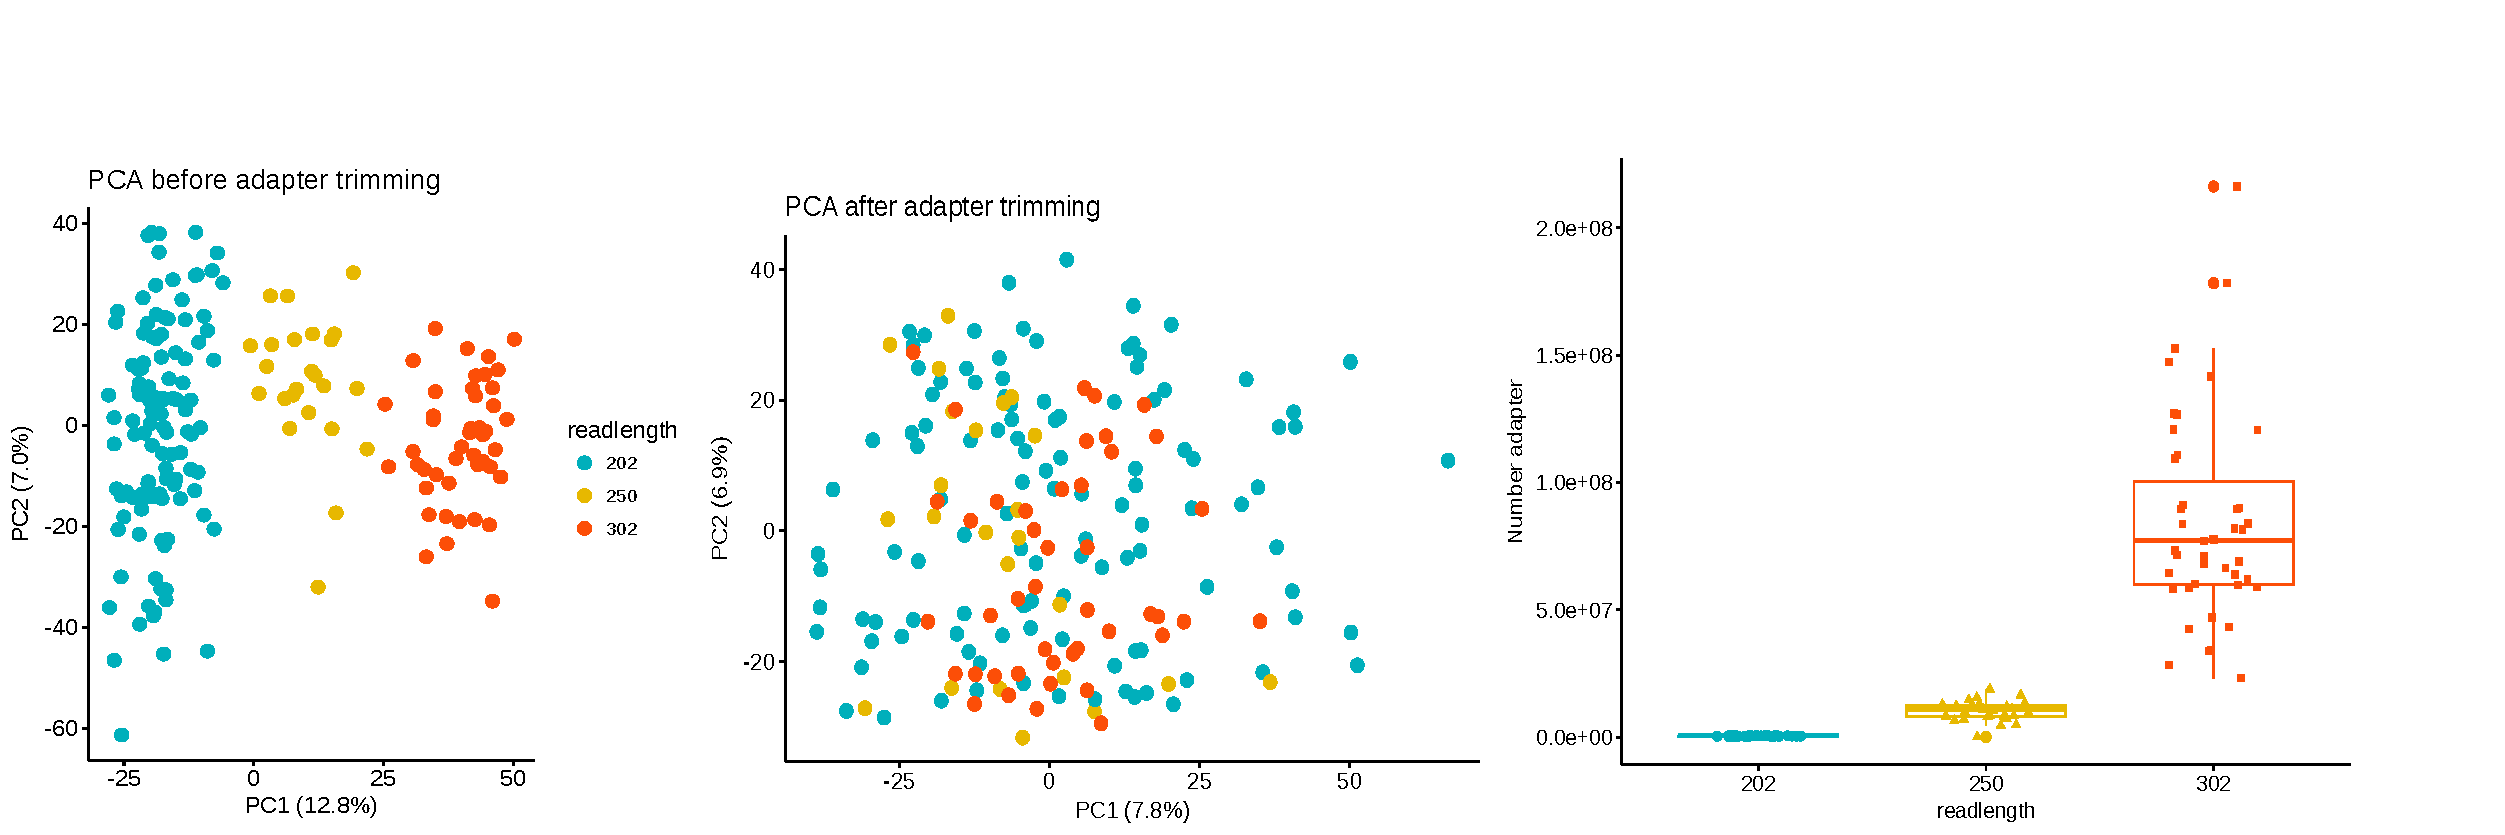
\includegraphics[width=\textwidth]{/home/almut/Dokumente/git/Transcriptome_CLL/thesis/Figures/pca_readlengthOld.pdf}
		\end{subfigure}
		%\quad
		%\begin{subfigure}[t]{0.3\columnwidth}
		%	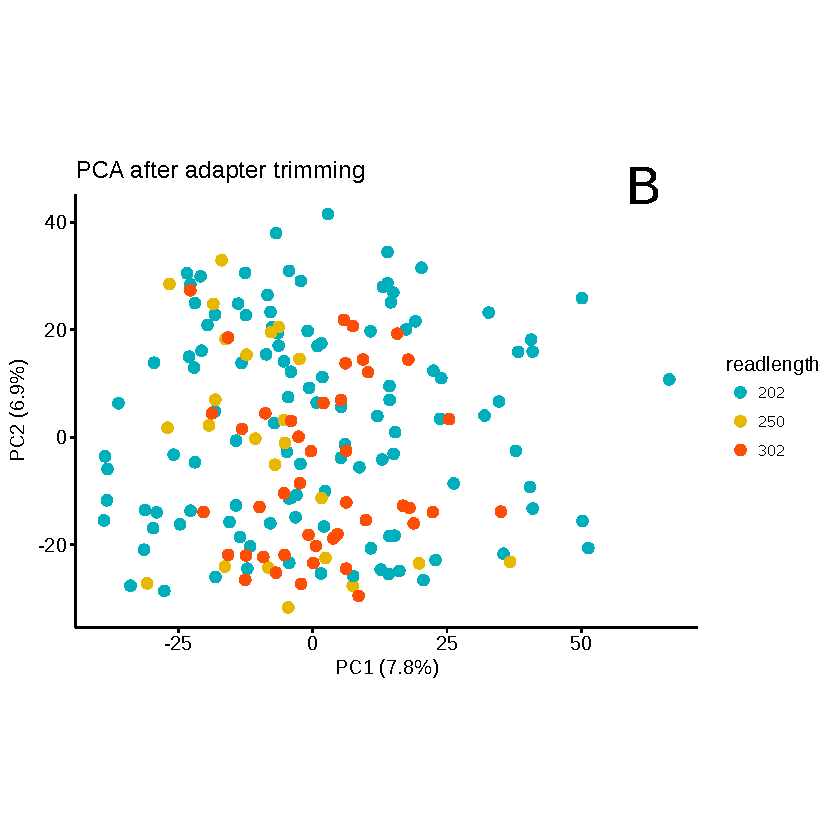
\includegraphics[width=\textwidth]{/home/almut/Dokumente/git/Transcriptome_CLL/thesis/Figures/pca_readlengthtrimmed.pdf}
		%\end{subfigure}
	\end{figure}
\end{frame}
%
%
\begin{frame}[c]
	\frametitle{Methylation groups}
	\begin{figure}
		\centering
		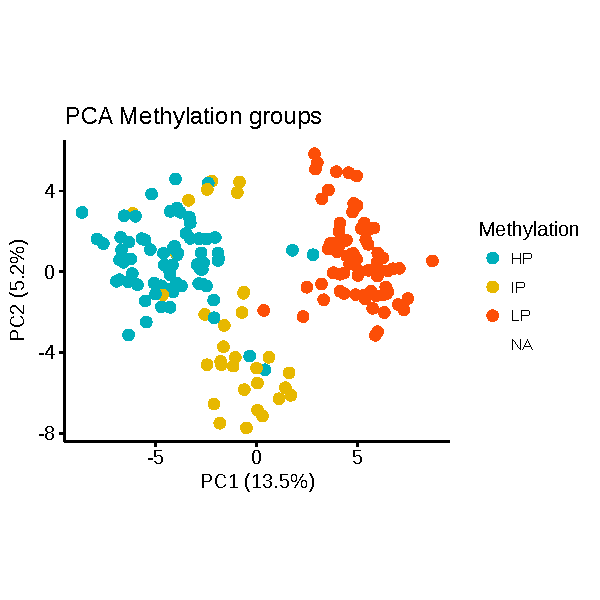
\includegraphics[width=0.7\textwidth]{/home/almut/Dokumente/git/Transcriptome_CLL/thesis/Figures/pca_Meth_top150.pdf}
	\end{figure}
\end{frame}
%
%
\begin{frame}[c]
	\frametitle{Methylation signature}
	\begin{figure}
		\centering
		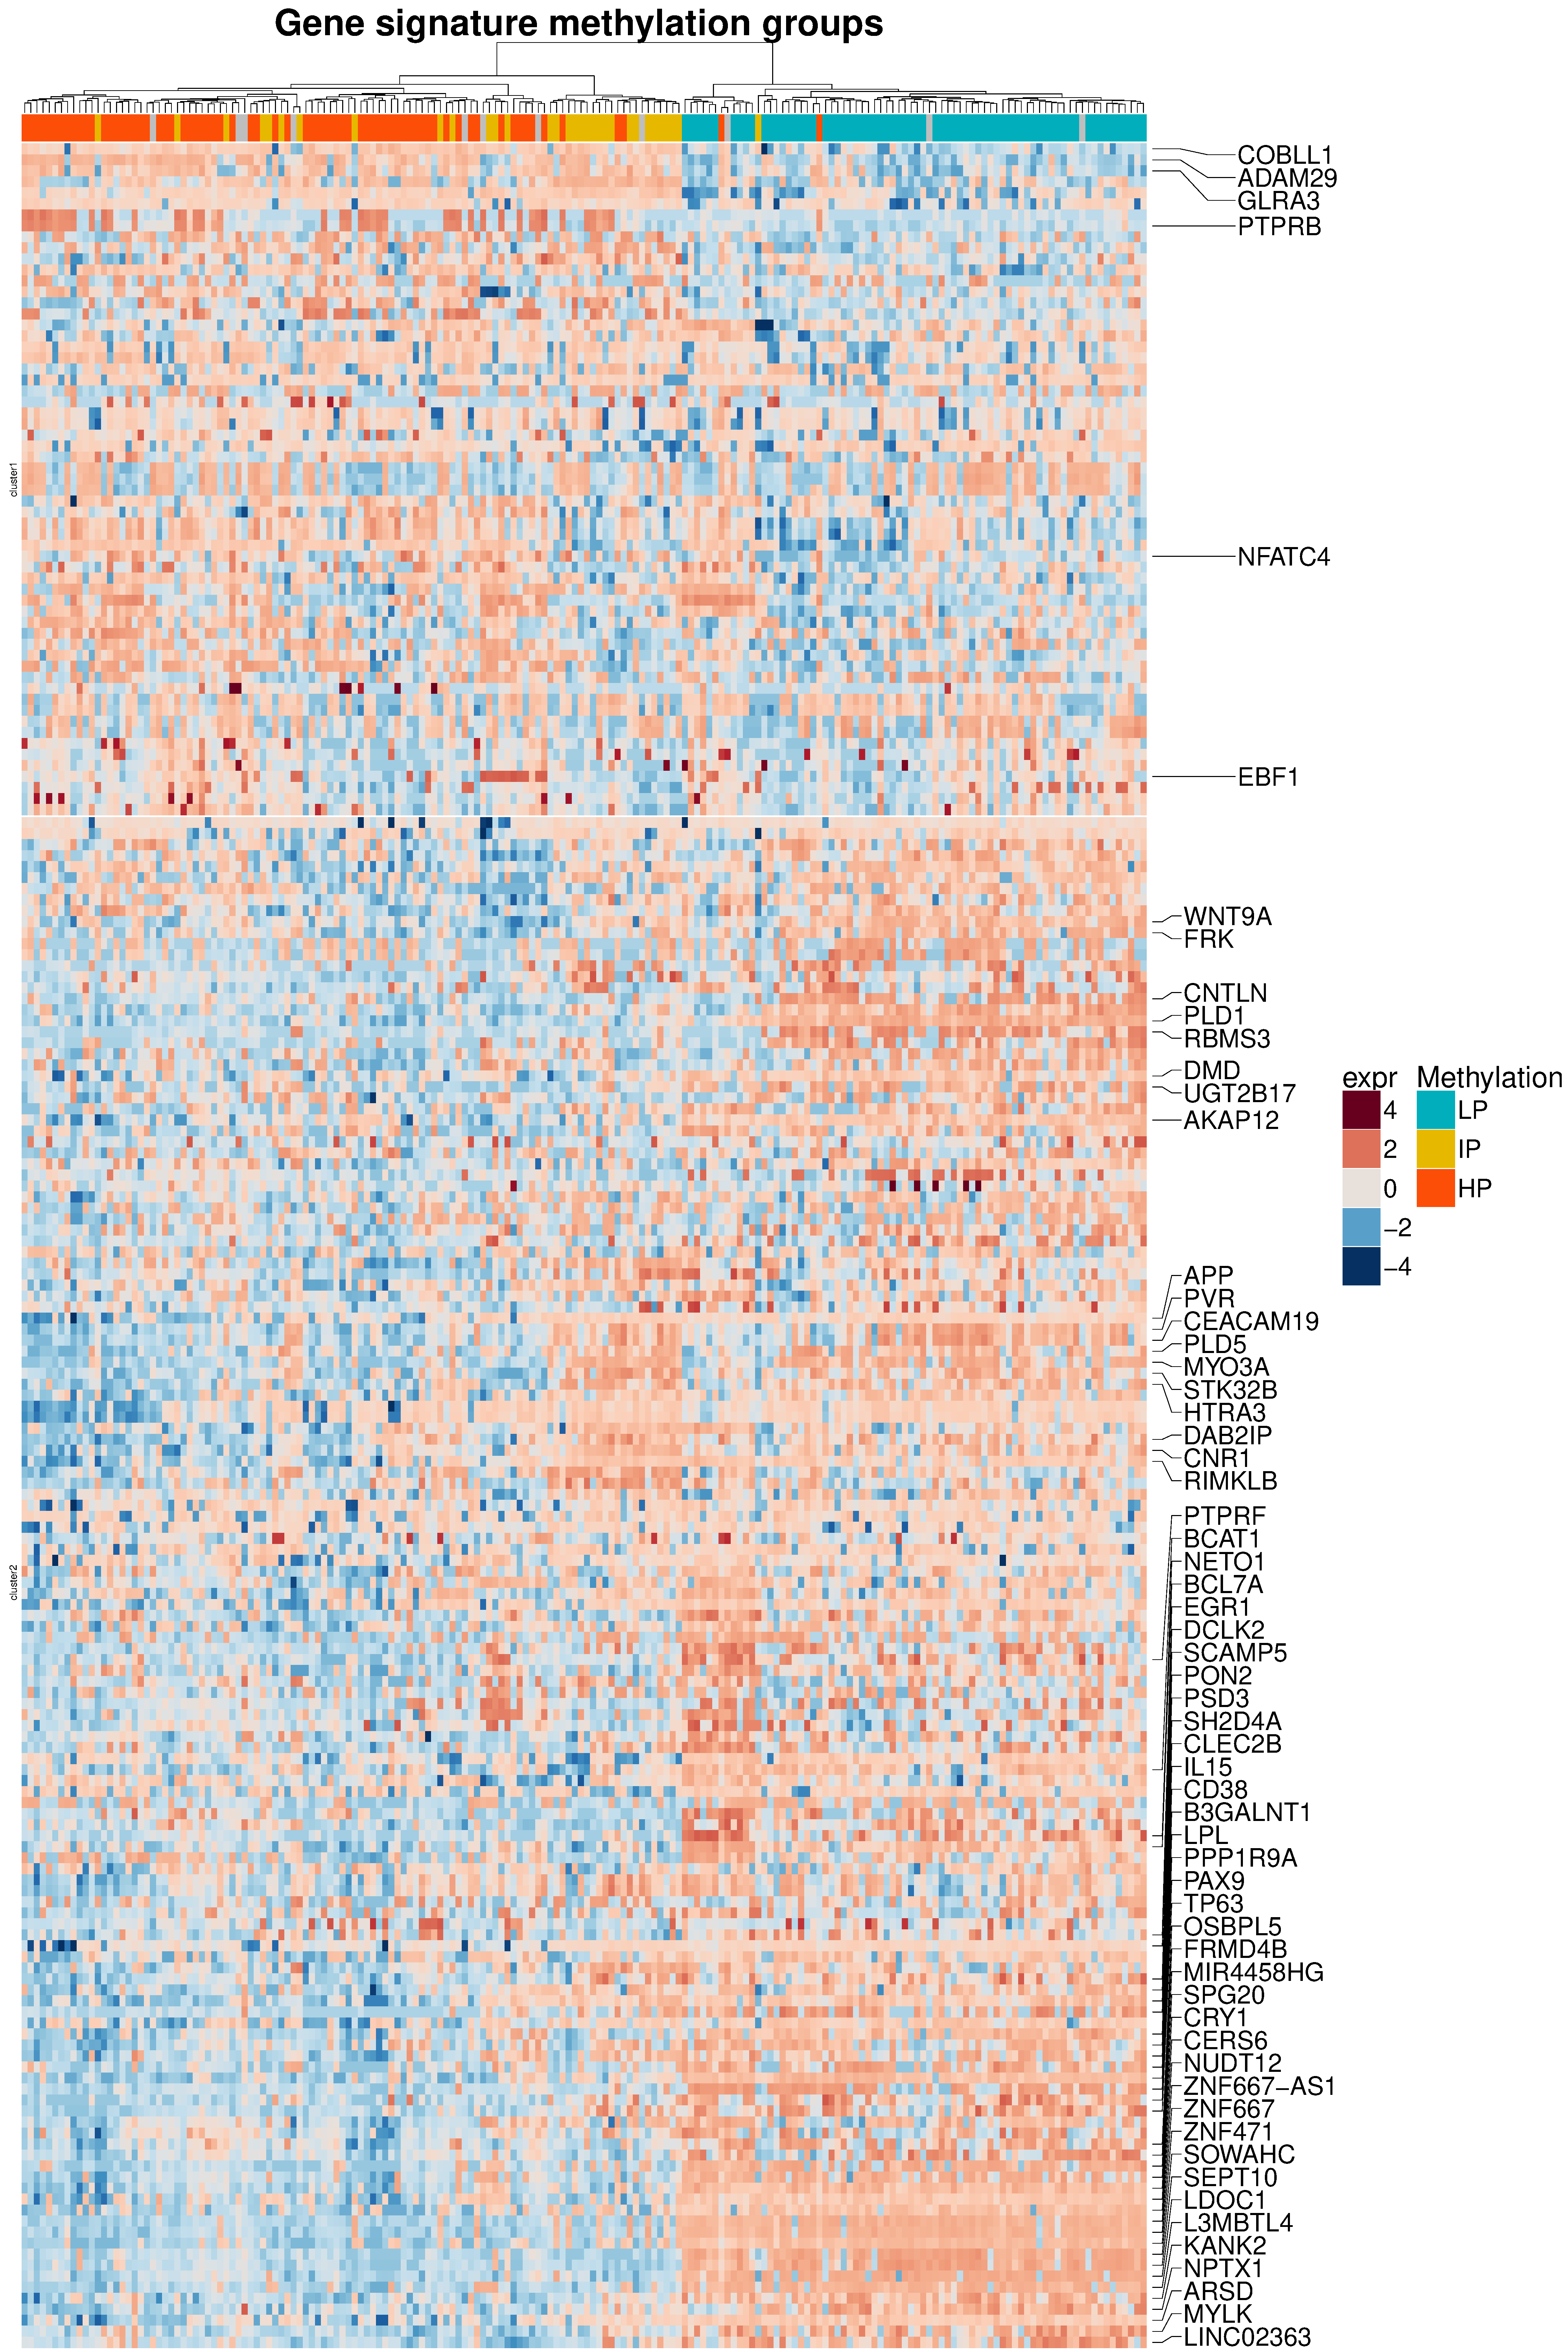
\includegraphics[width=0.5\textwidth]{/home/almut/Dokumente/git/Transcriptome_CLL/thesis/Figures/gene_expr_Methylationgroups_top150.pdf}
	\end{figure}
\end{frame}
%
%
\begin{frame}[c]
	\frametitle{TP53/Del17p13}
	\begin{figure}
		\centering
		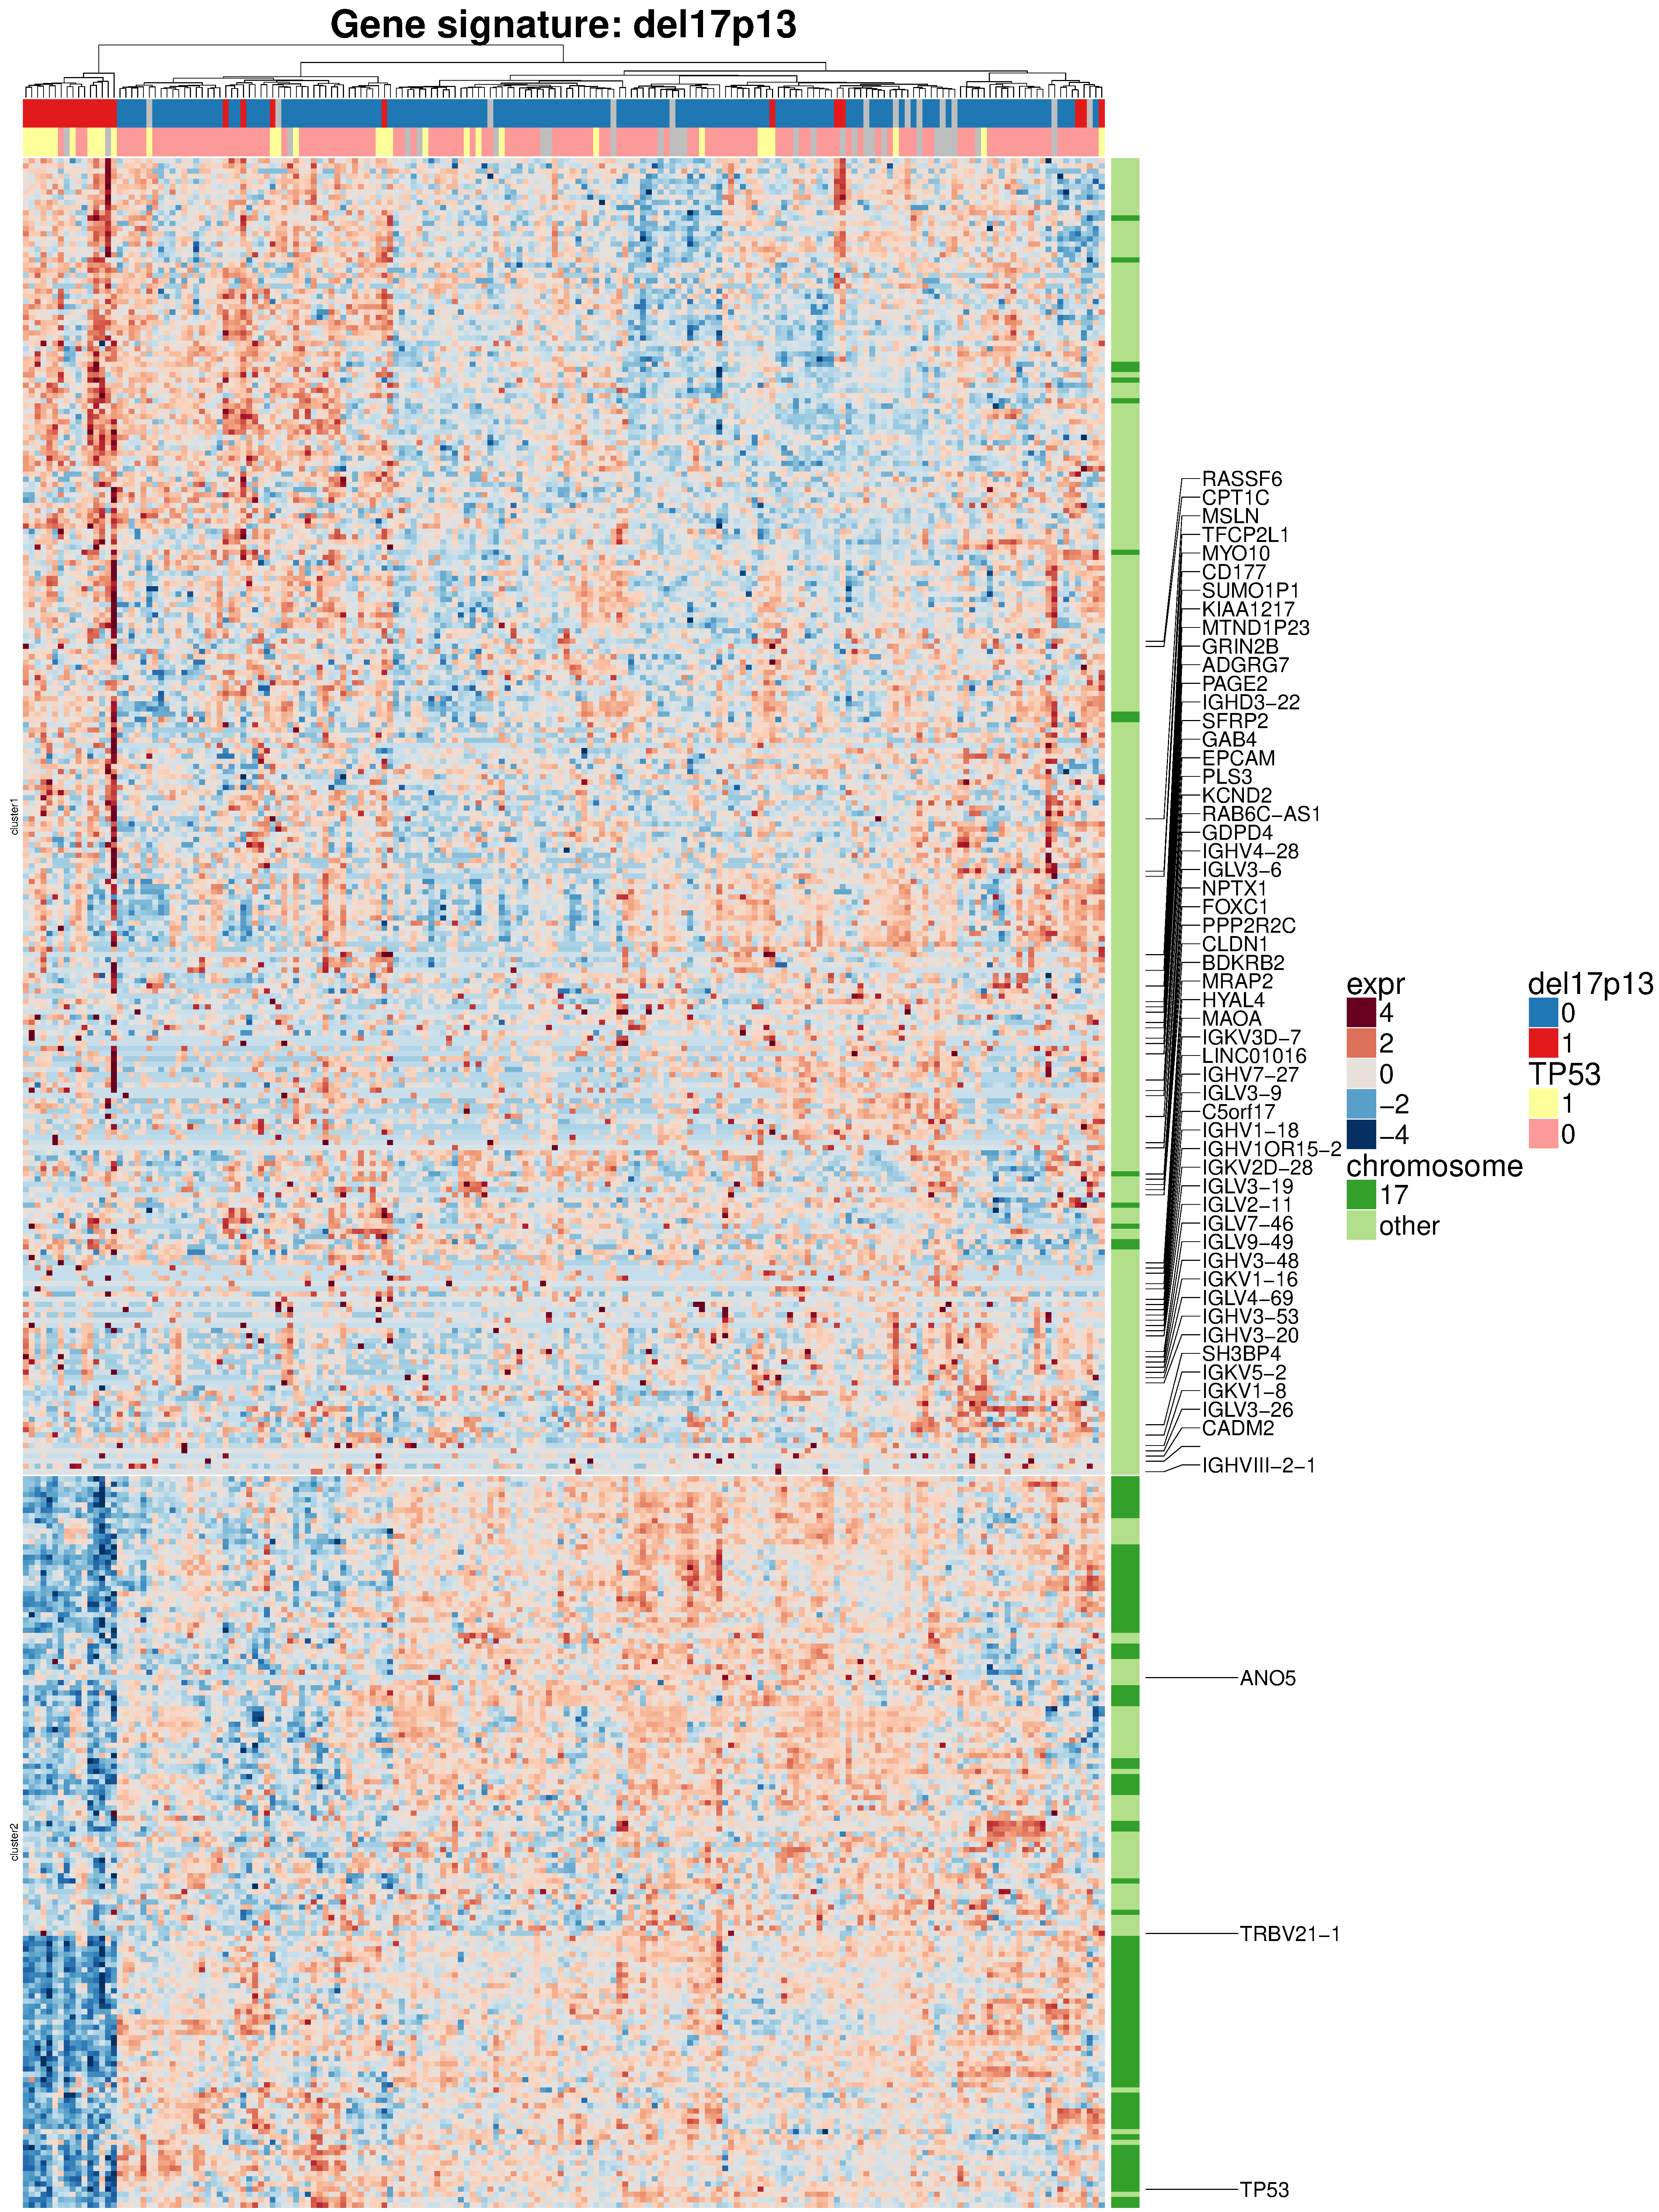
\includegraphics[width=0.6\textwidth]{/home/almut/Dokumente/git/Transcriptome_CLL/thesis/Figures/gene_exprDel17p13_gsea_Kegg.pdf}
	\end{figure}
\end{frame}
%
%
\begin{frame}[c]
	\frametitle{SF3B1 signature}
	\begin{figure}
		\centering
		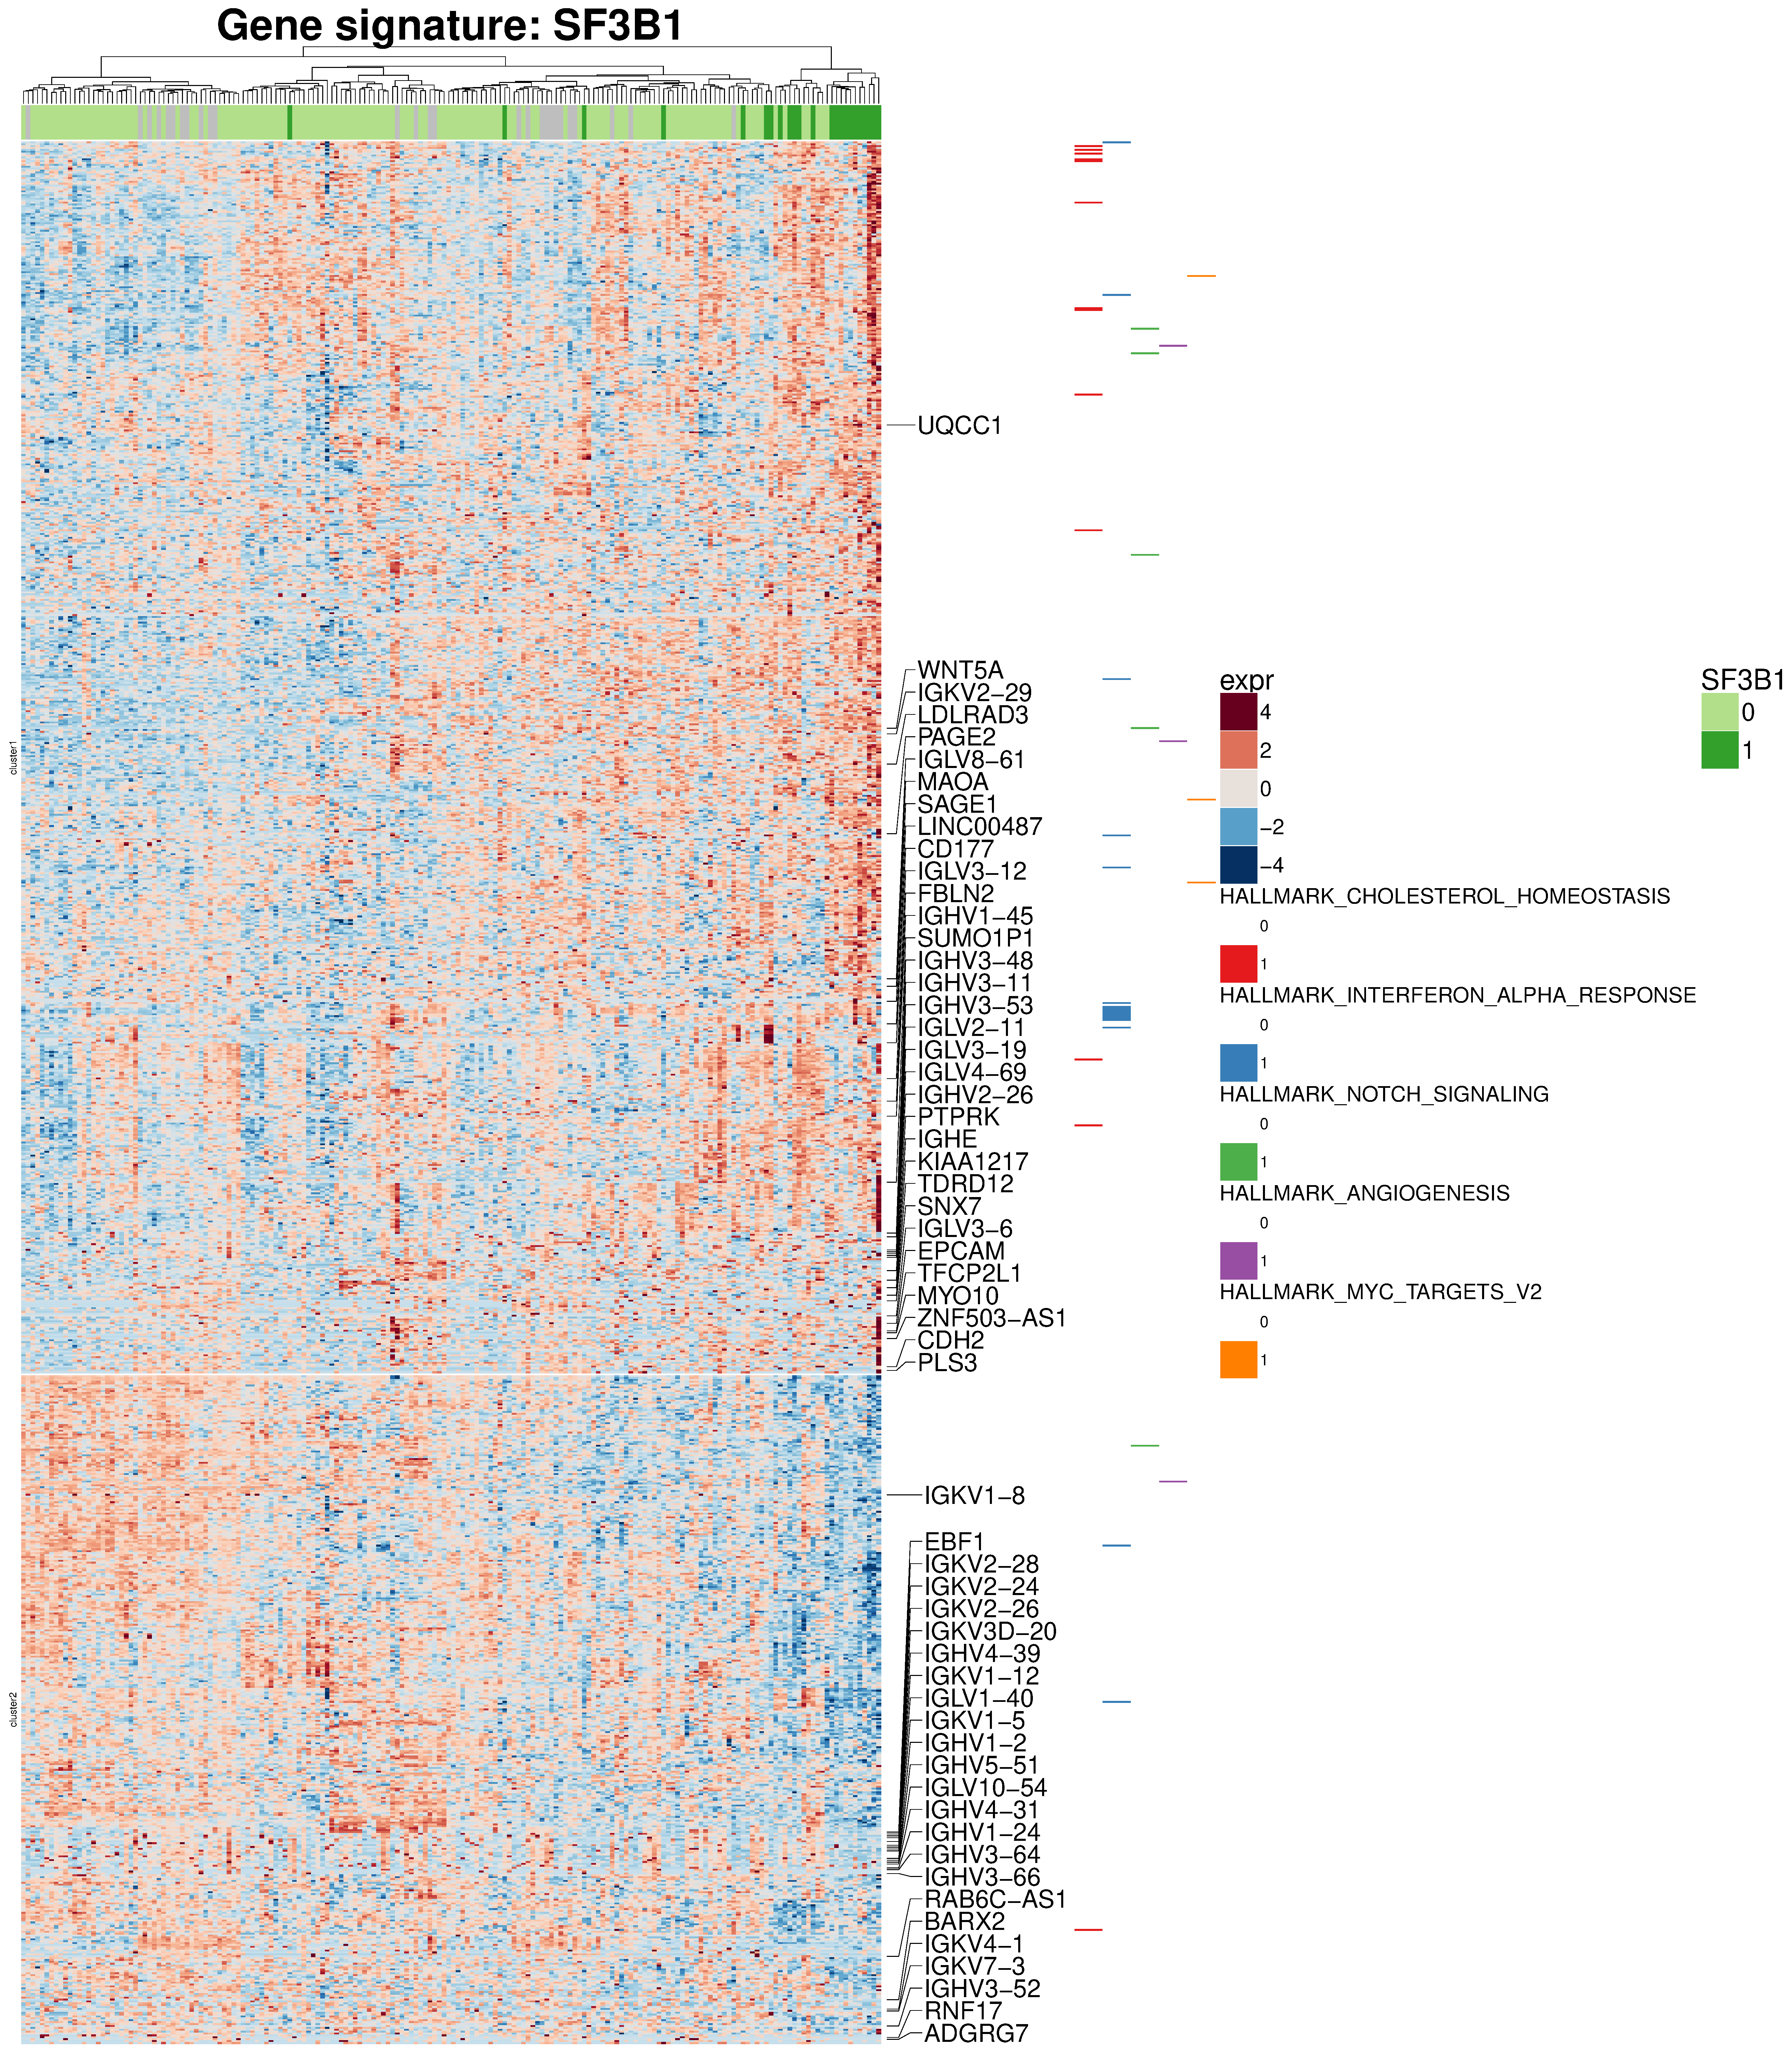
\includegraphics[width=0.58\textwidth]{/home/almut/Dokumente/git/Transcriptome_CLL/thesis/Figures/gene_exprSF3B1_gsea_Hallmark.pdf}
	\end{figure}
\end{frame}
%
%
\begin{frame}[c]
	\frametitle{Del13q14 signature}
	\begin{figure}
		\centering
		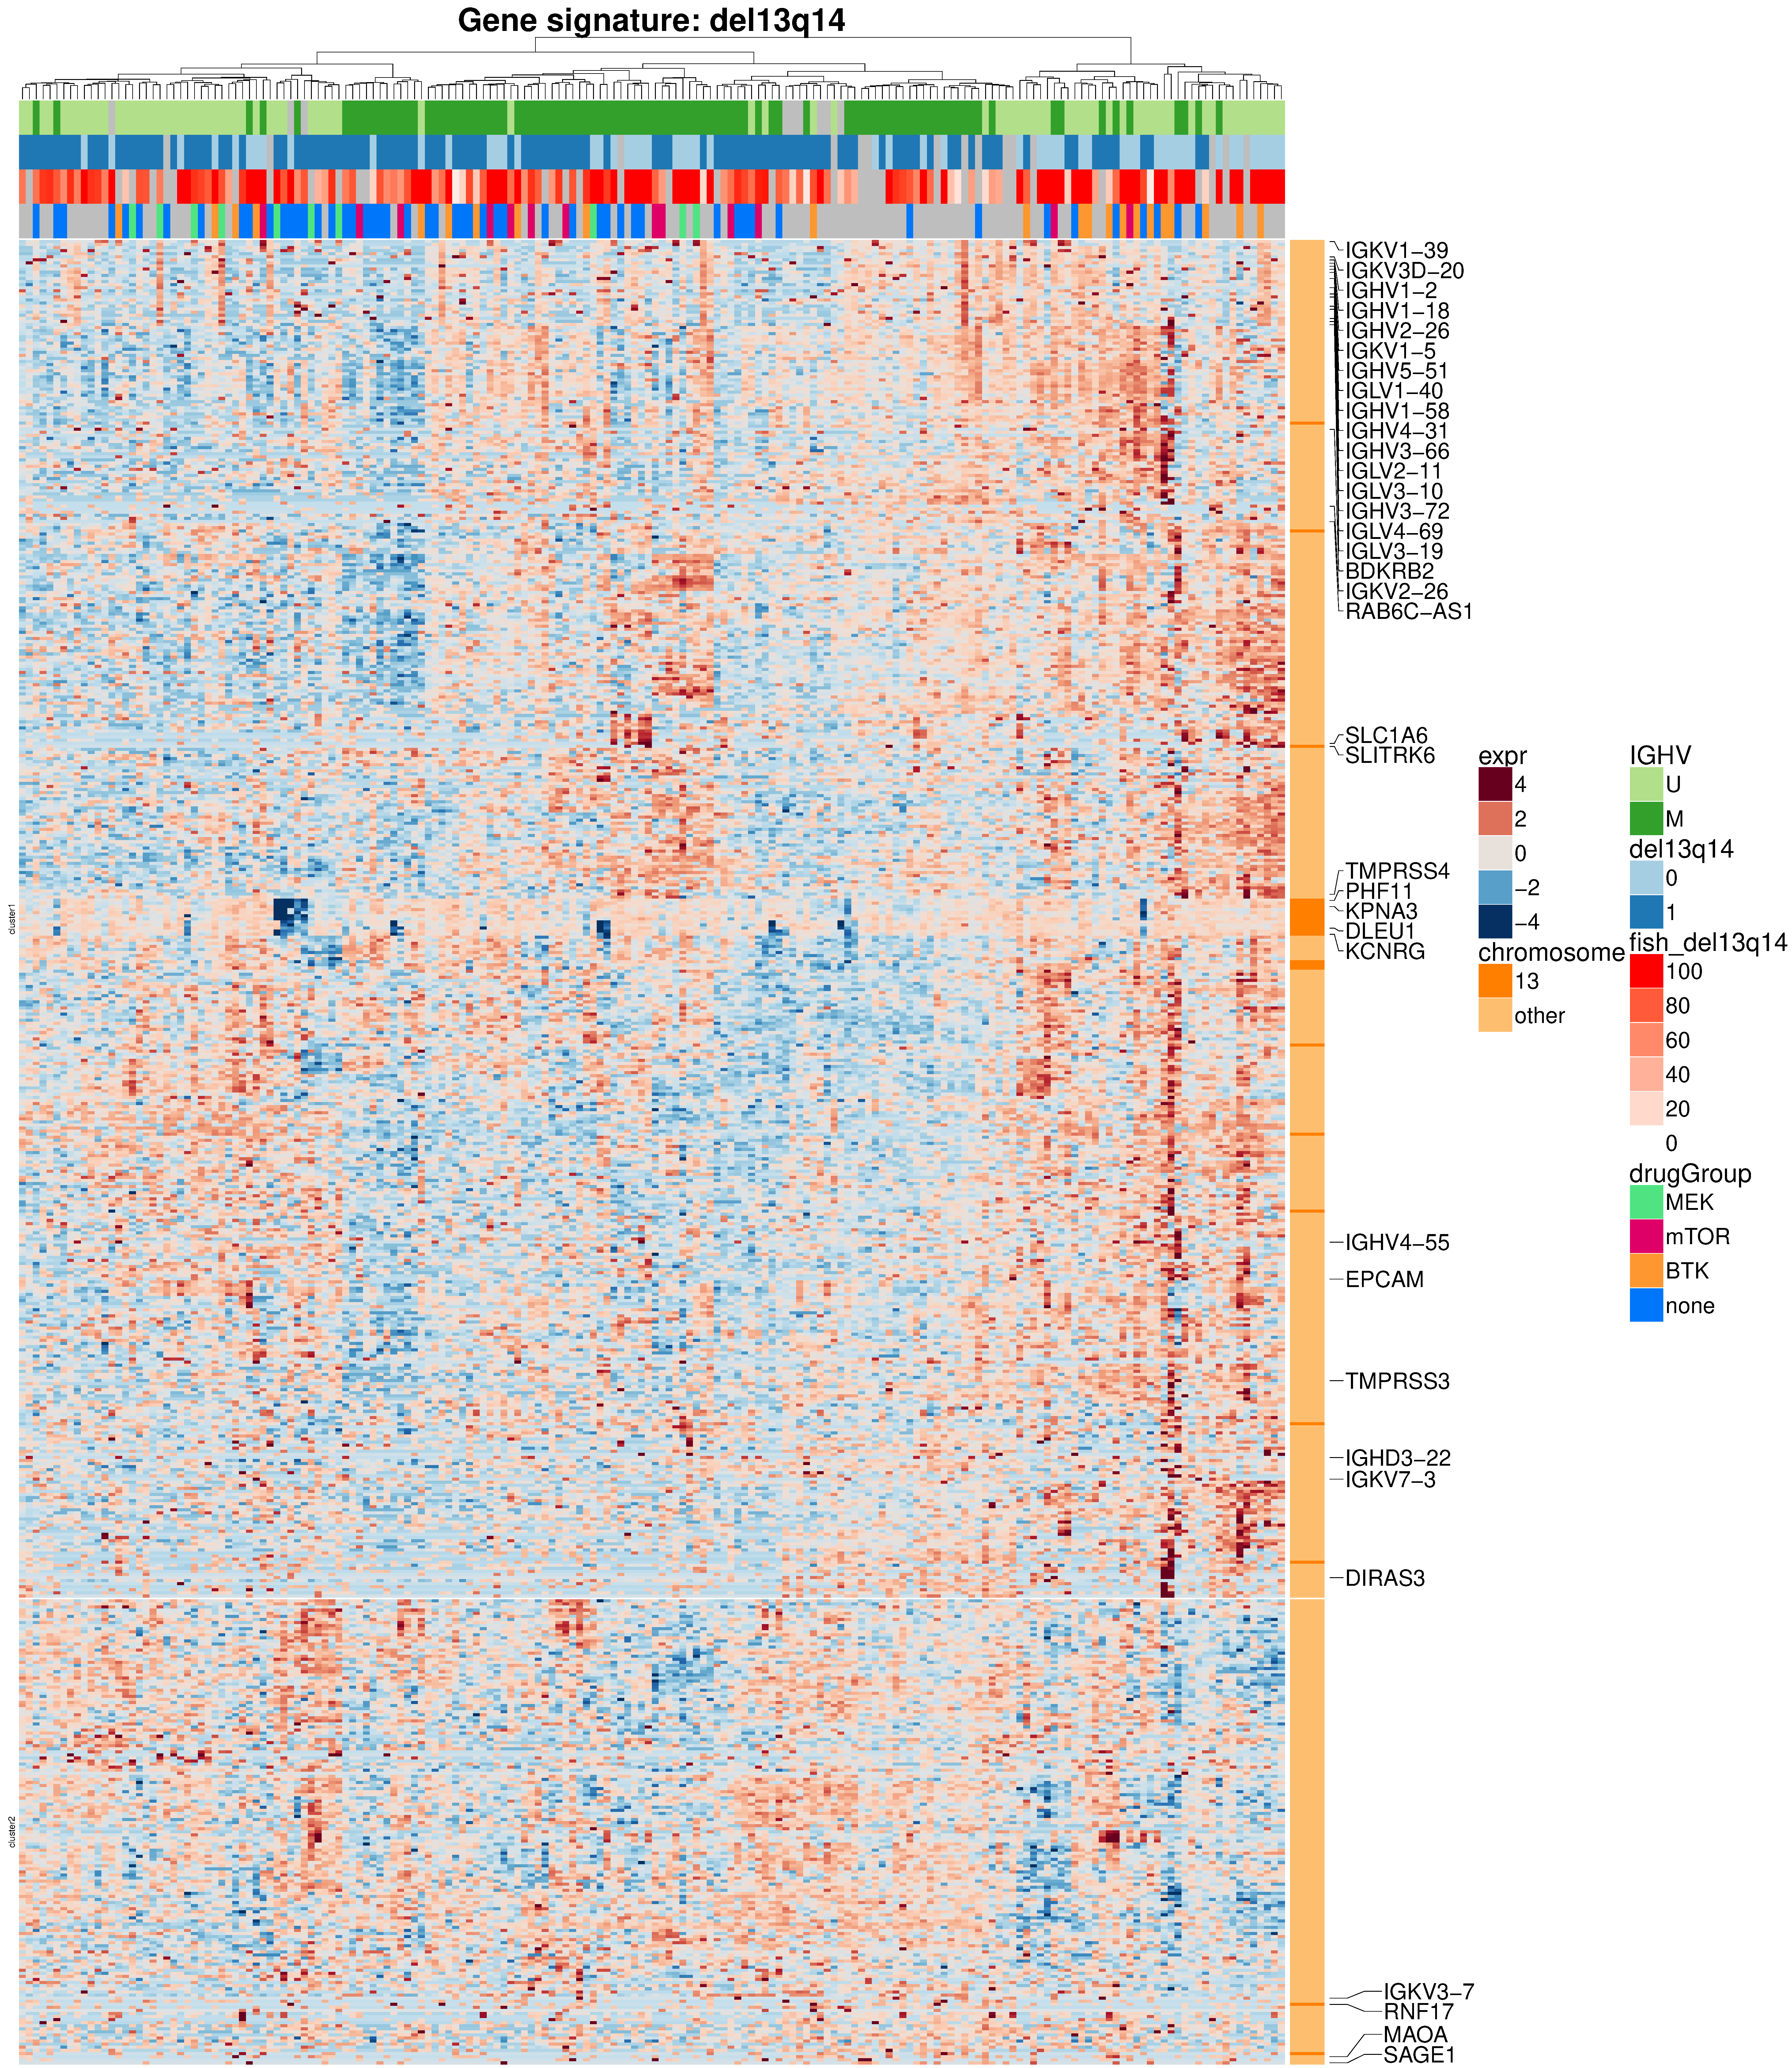
\includegraphics[width=0.65\textwidth]{/home/almut/Dokumente/git/Transcriptome_CLL/thesis/Figures/gene_exprDel13q14_gsea_Kegg.pdf}
	\end{figure}
\end{frame}
%
%
\begin{frame}[c]
	\frametitle{Del11q22 signature}
	\begin{figure}
		\centering
		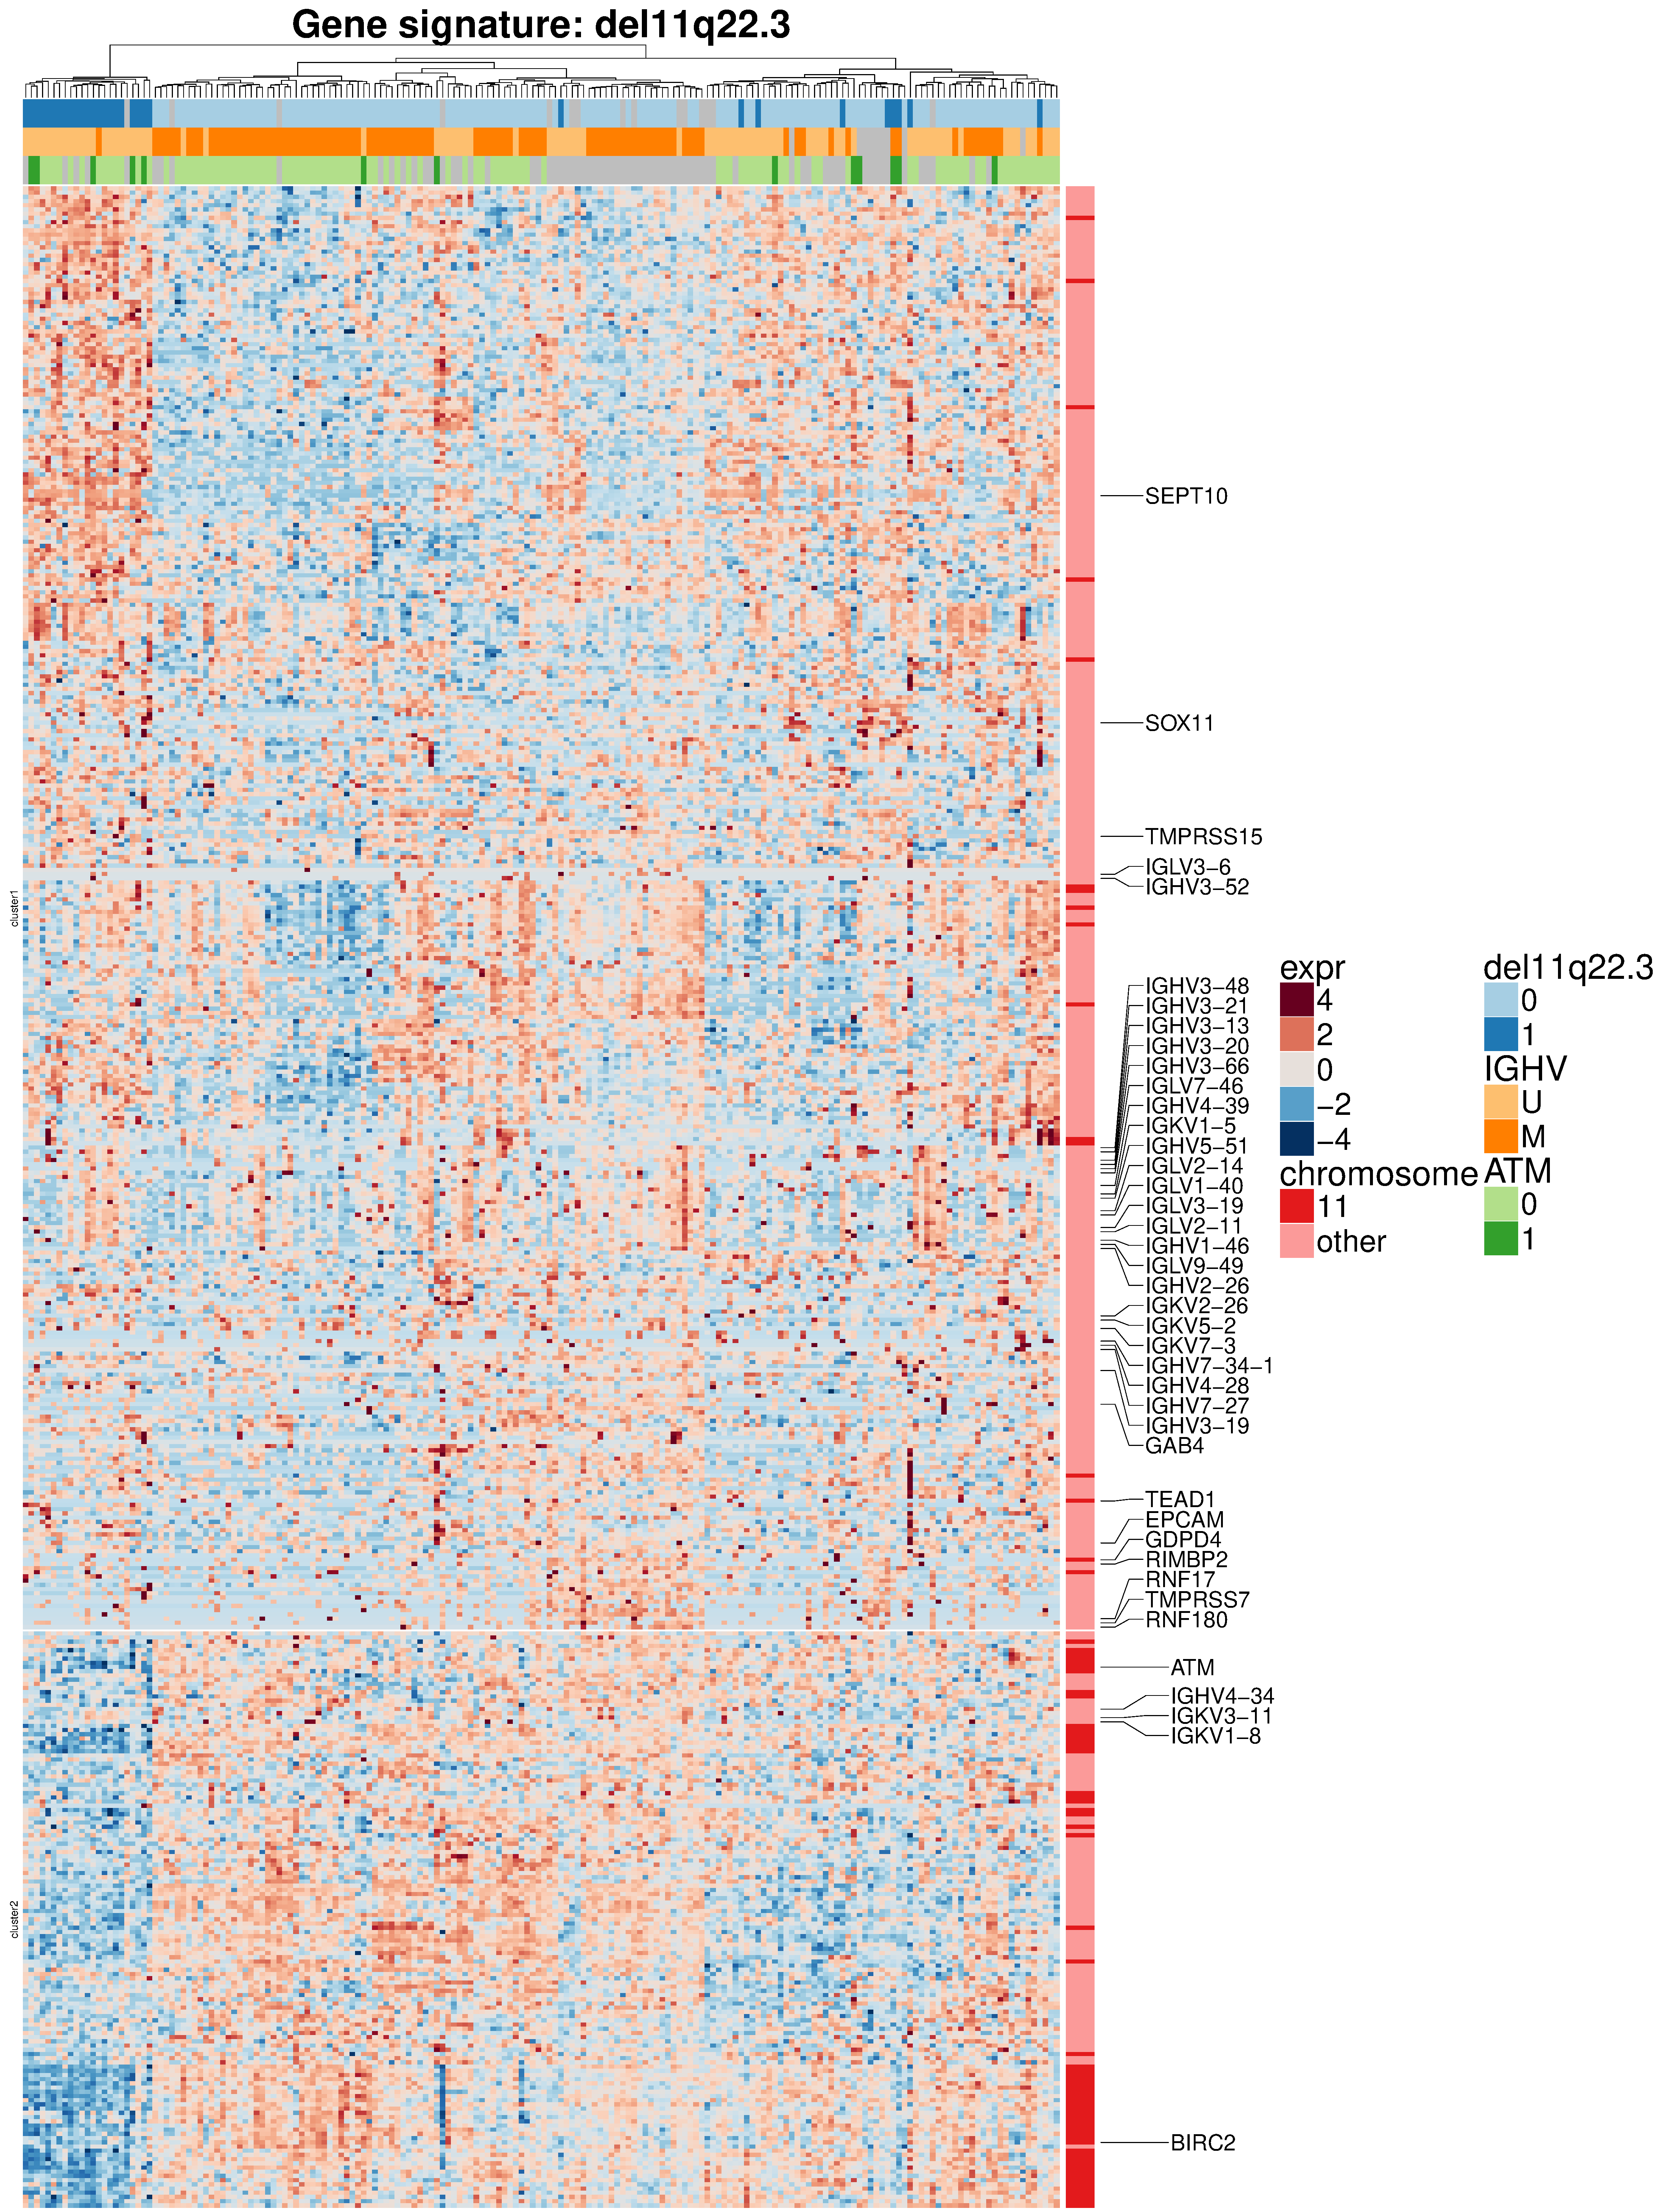
\includegraphics[width=0.6\textwidth]{/home/almut/Dokumente/git/Transcriptome_CLL/thesis/Figures/gene_exprdel11q22_gsea_Hallmark.pdf}
	\end{figure}
\end{frame}
%
% 
\begin{frame}[c]
	\frametitle{BRAF signature}
	\begin{figure}
		\centering
		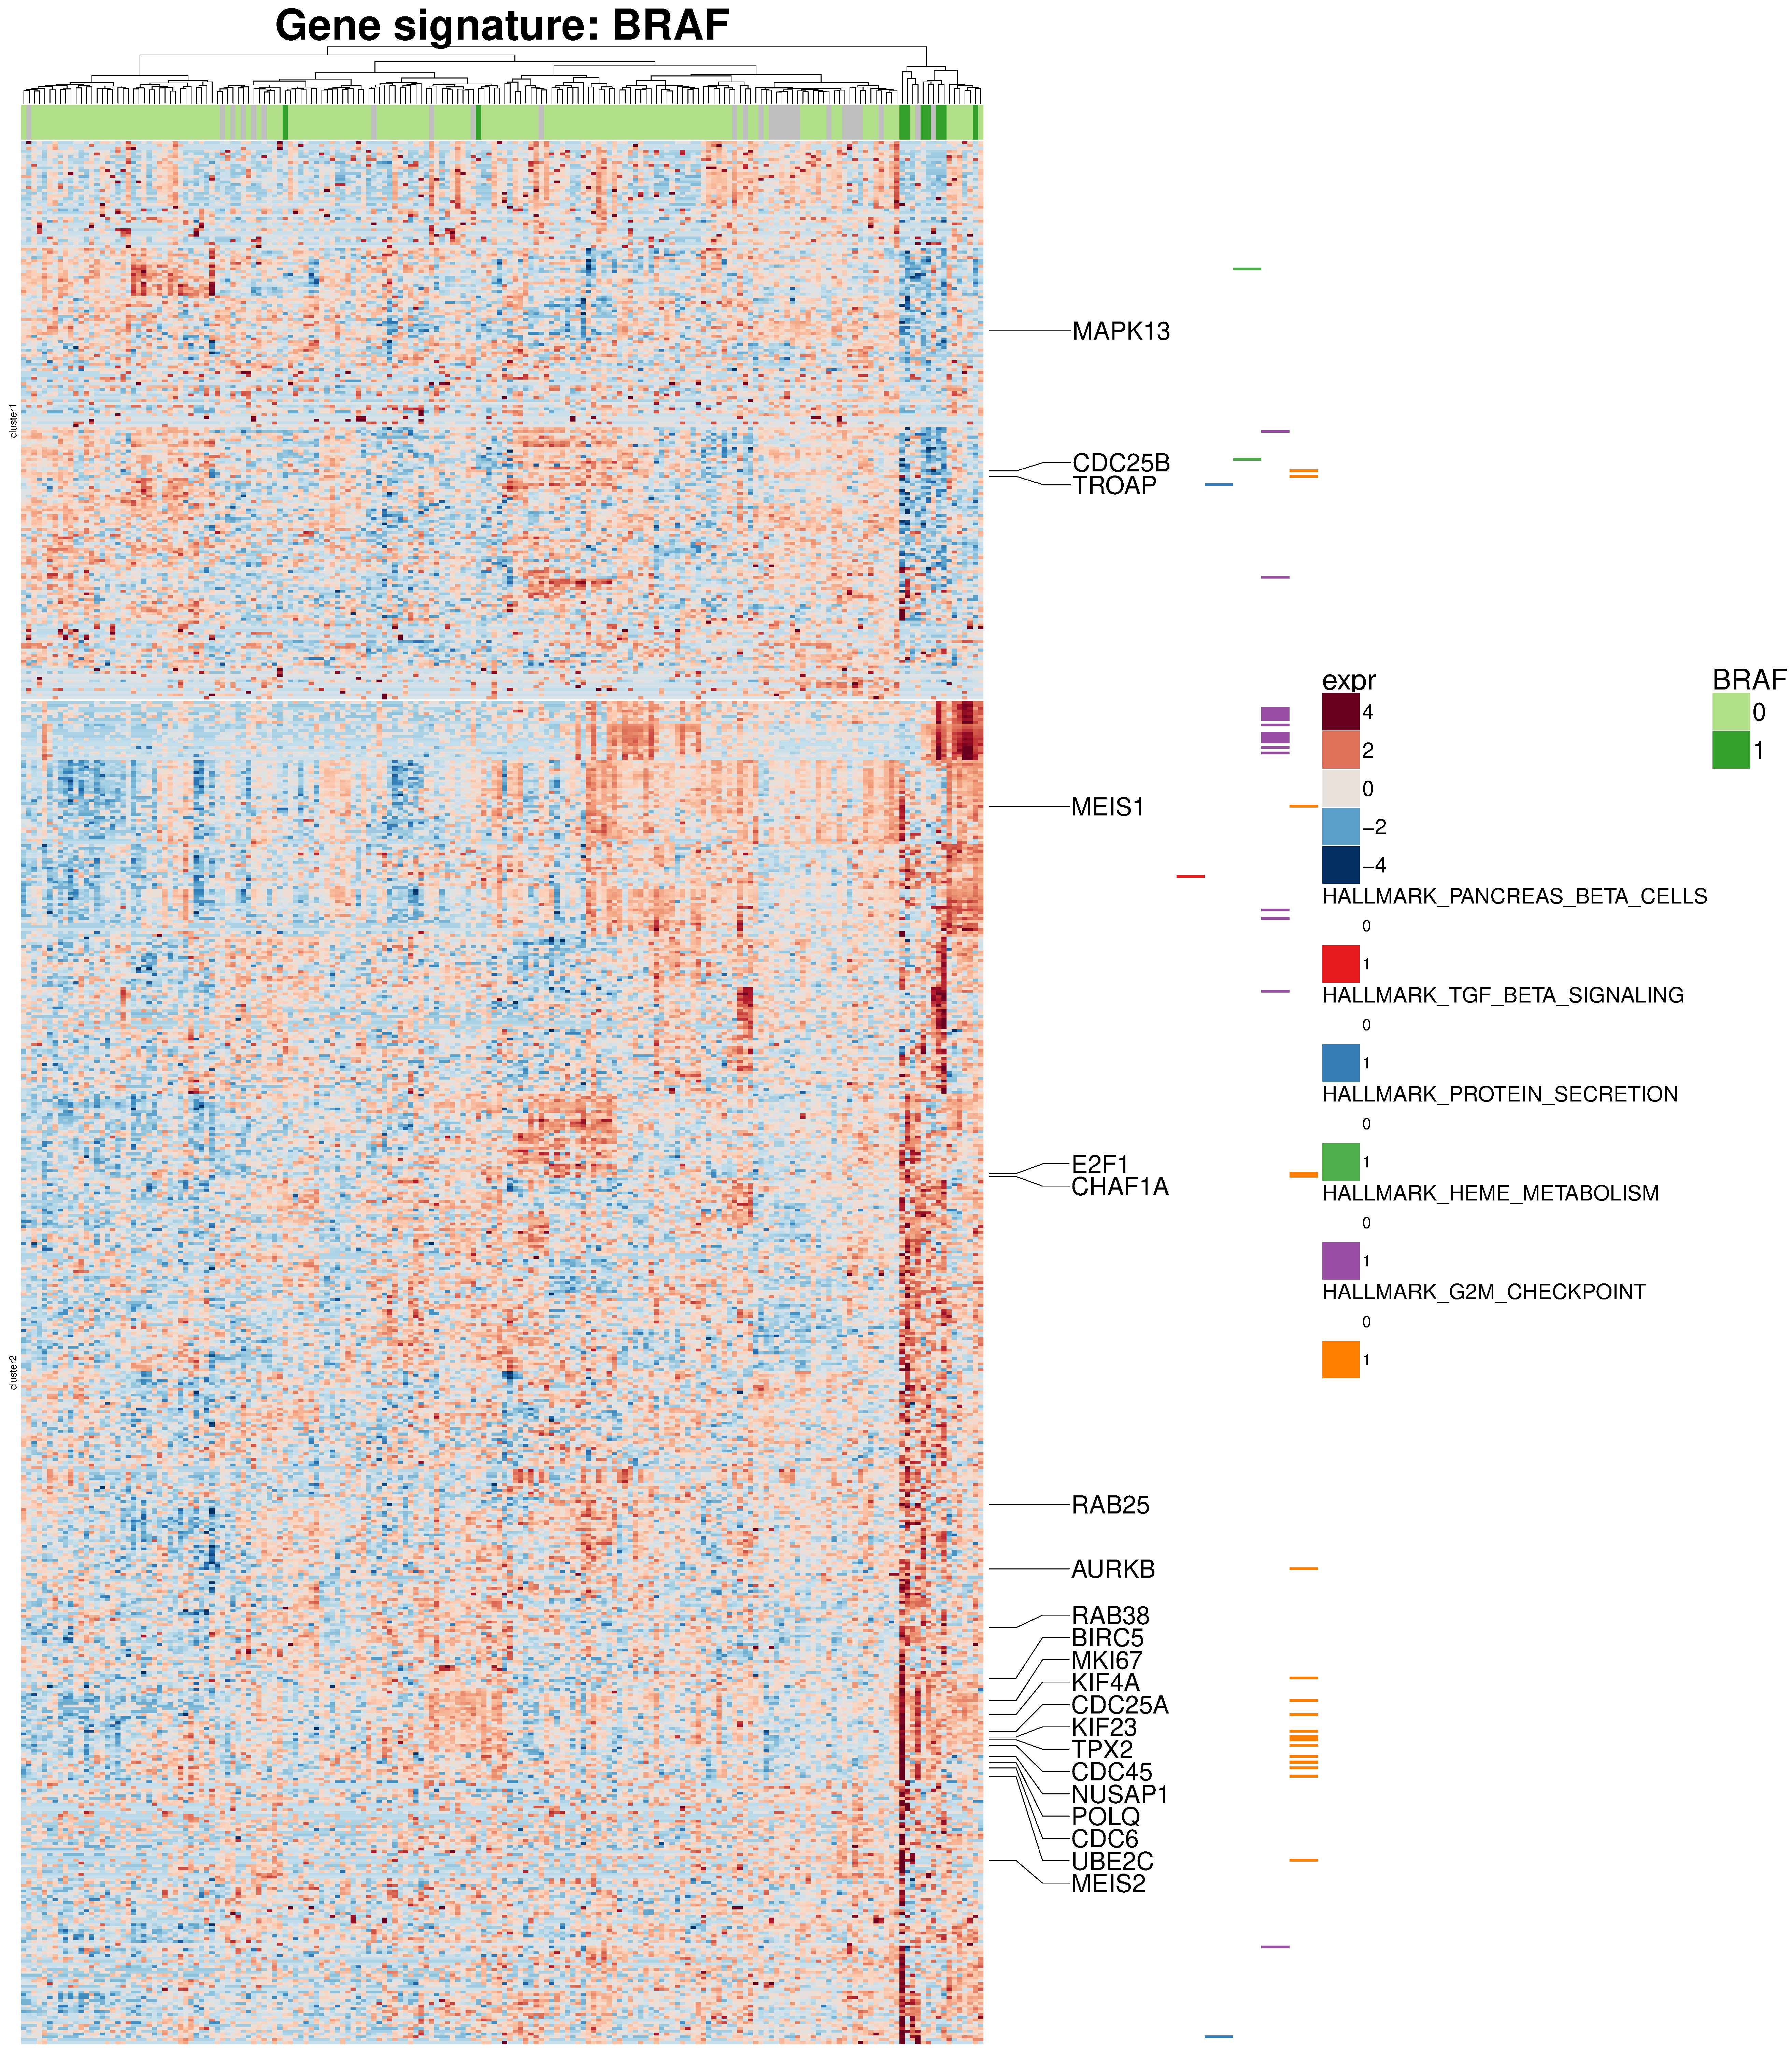
\includegraphics[width=0.7\textwidth]{/home/almut/Dokumente/git/Transcriptome_CLL/thesis/Figures/gene_exprBRAF_gsea_Hallmark.pdf}
	\end{figure}
\end{frame}
%
% 
\begin{frame}[c]
	\frametitle{Notch signature}
	\begin{figure}
		\centering
		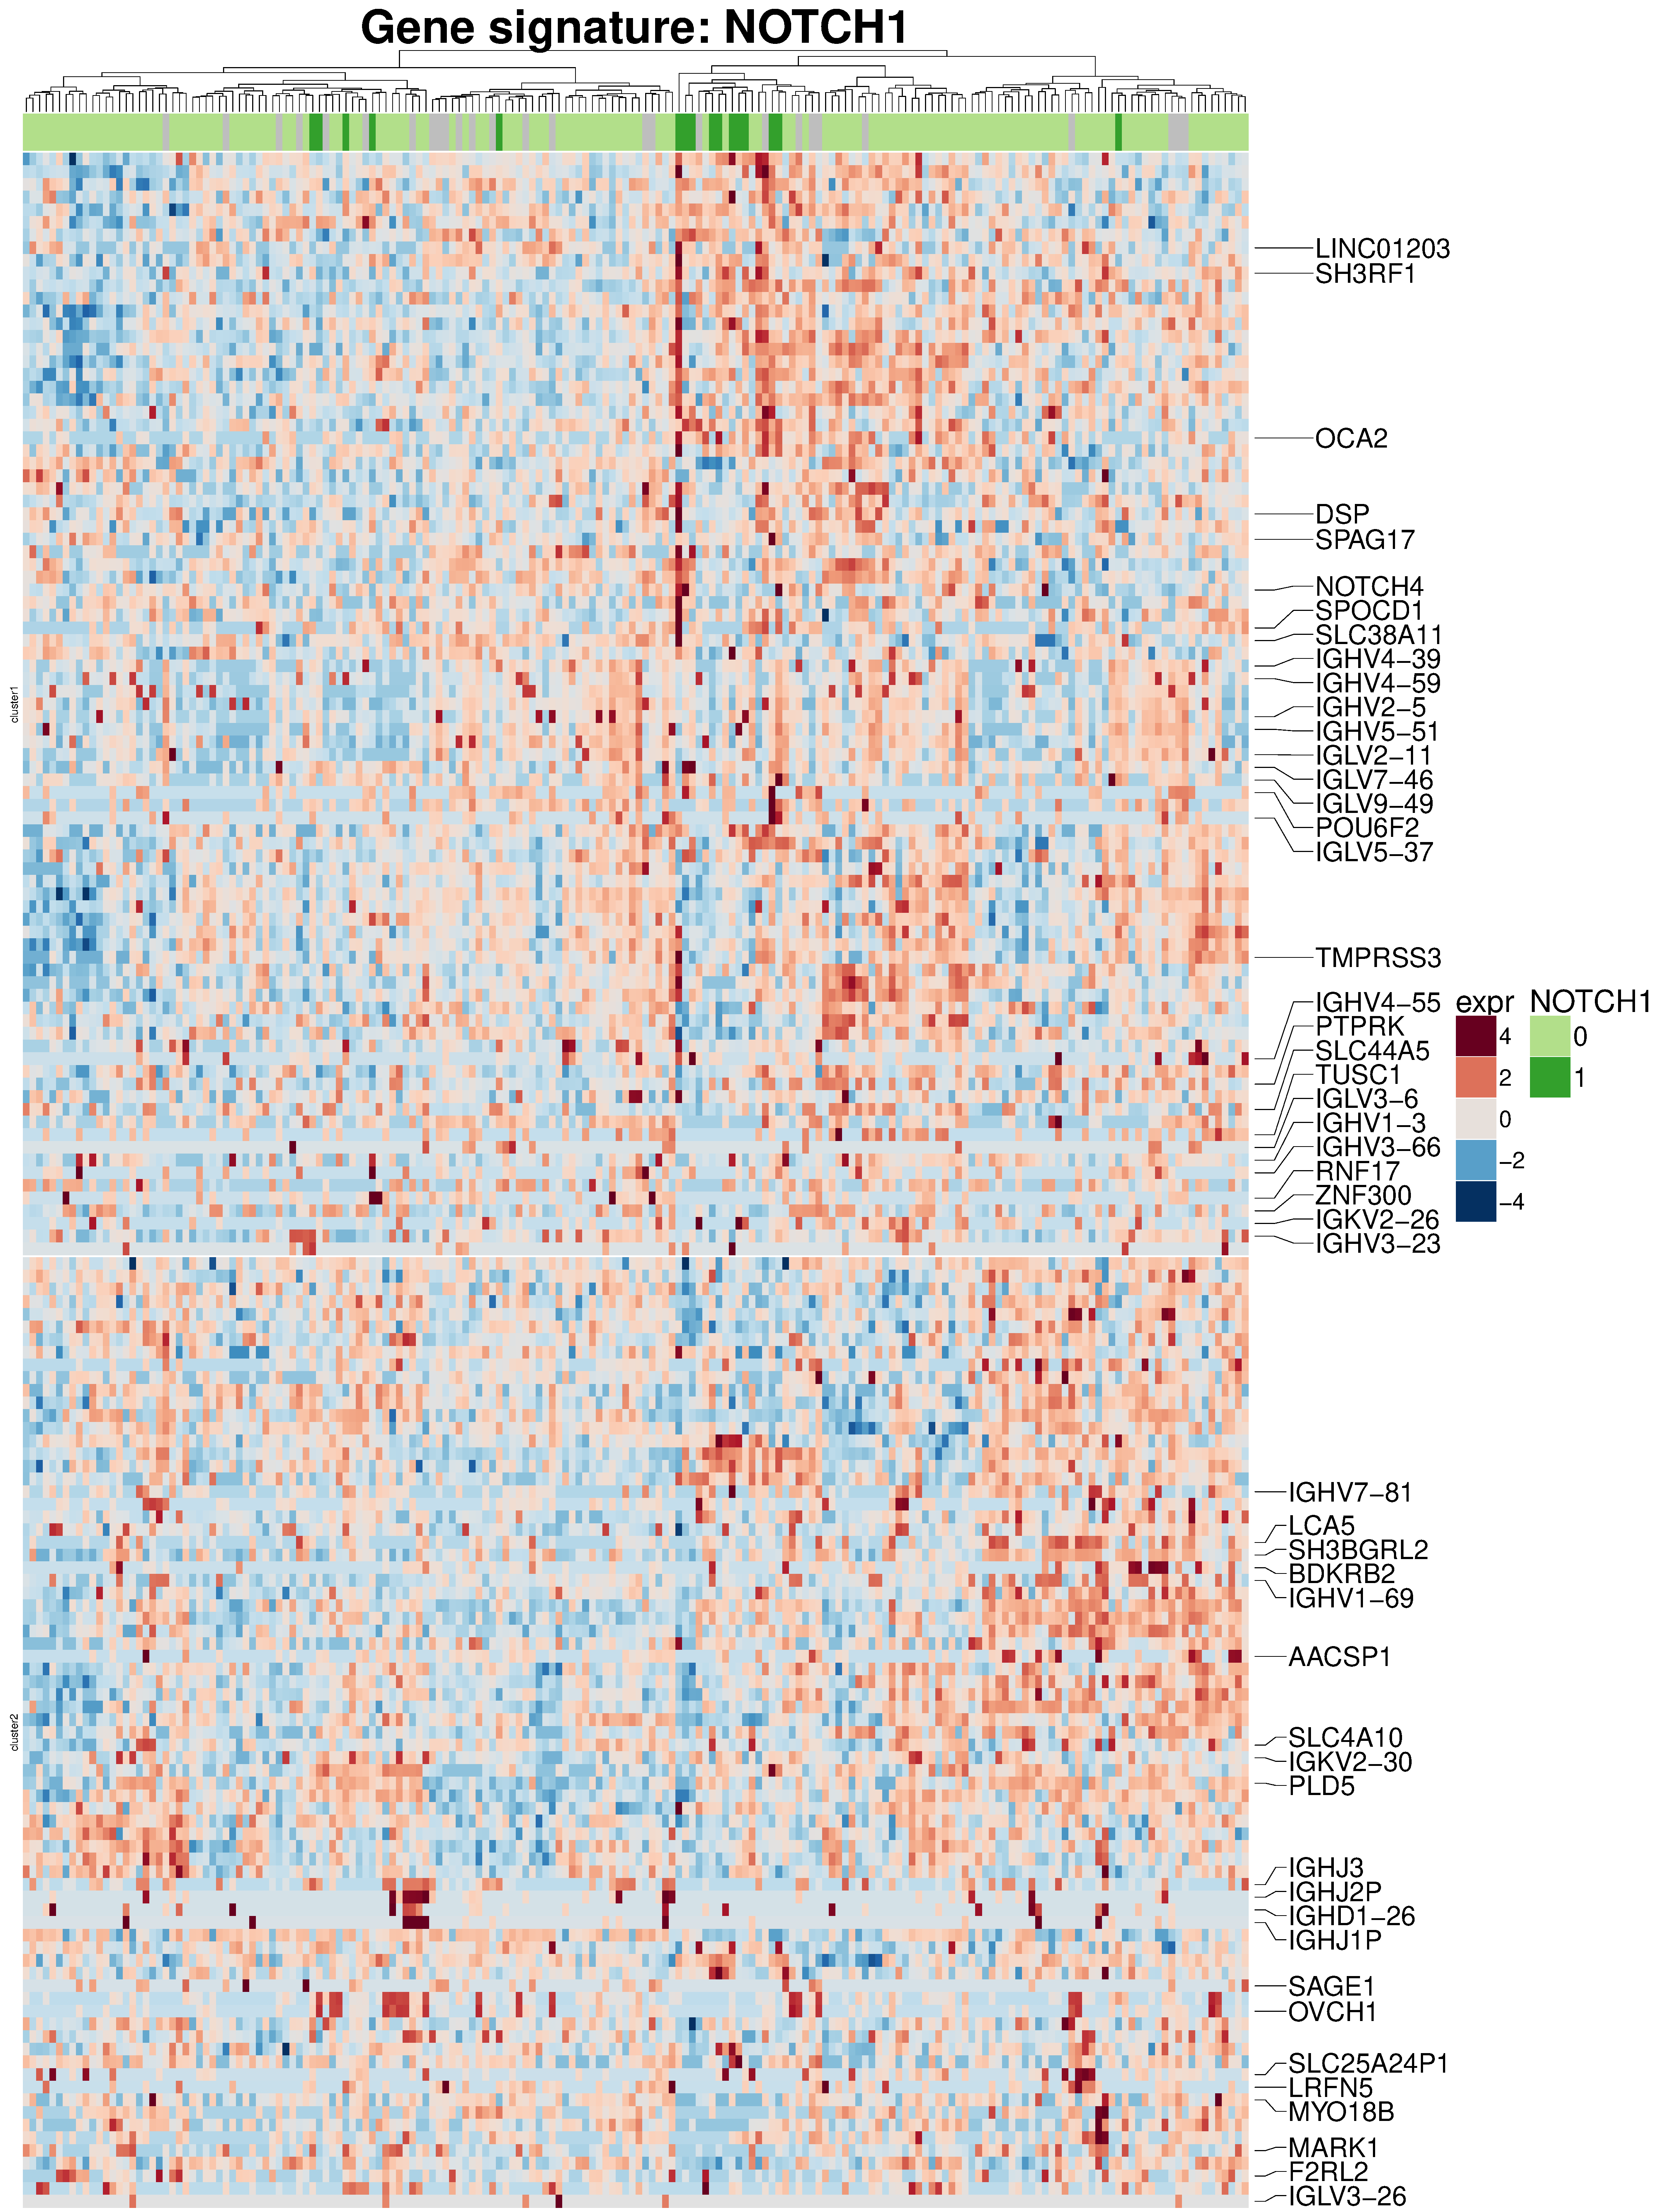
\includegraphics[width=0.5\textwidth]{/home/almut/Dokumente/git/Transcriptome_CLL/thesis/Figures/gene_exprNOTCH1_gsea_Hallmark.pdf}
	\end{figure}
\end{frame}
%
% 
\begin{frame}[c]
	\frametitle{Gain8q24 signature}
	\begin{figure}
		\centering
		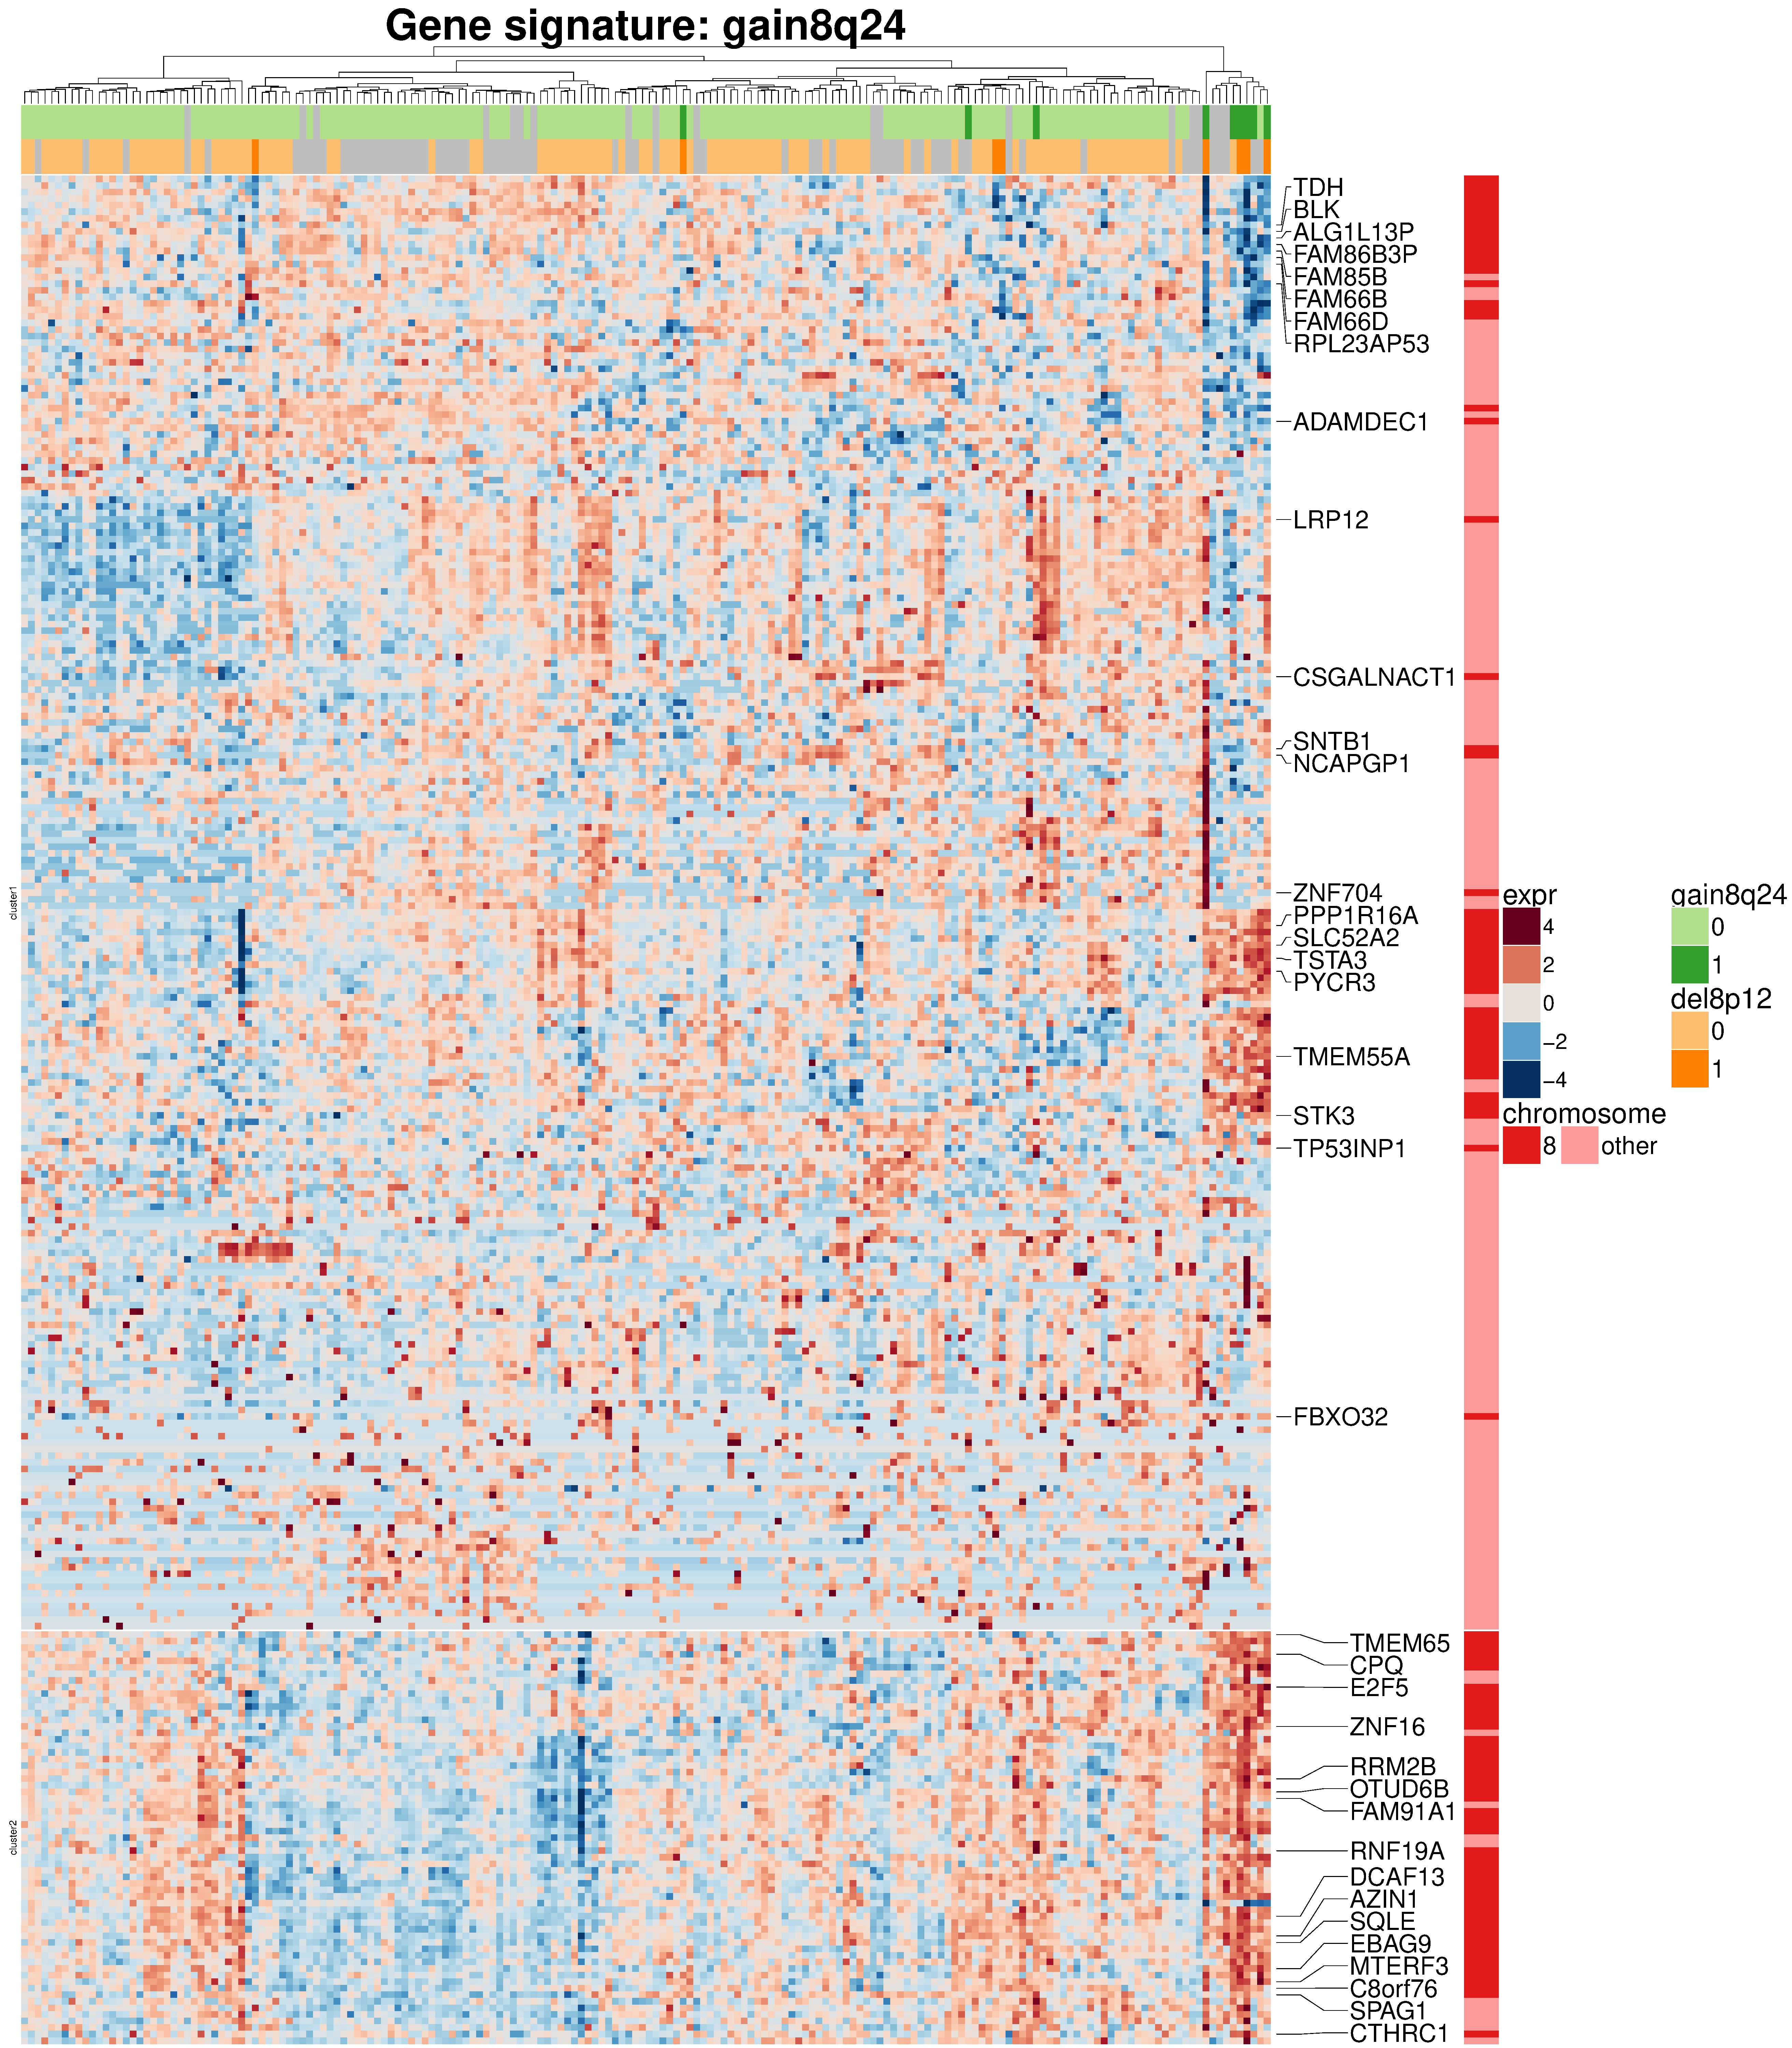
\includegraphics[width=0.6\textwidth]{/home/almut/Dokumente/git/Transcriptome_CLL/thesis/Figures/gene_exprgain8q24_gsea_Hallmark.pdf}
	\end{figure}
\end{frame}
%
% 
\begin{frame}[c]
	\frametitle{MED12 signature}
	\begin{figure}
		\centering
		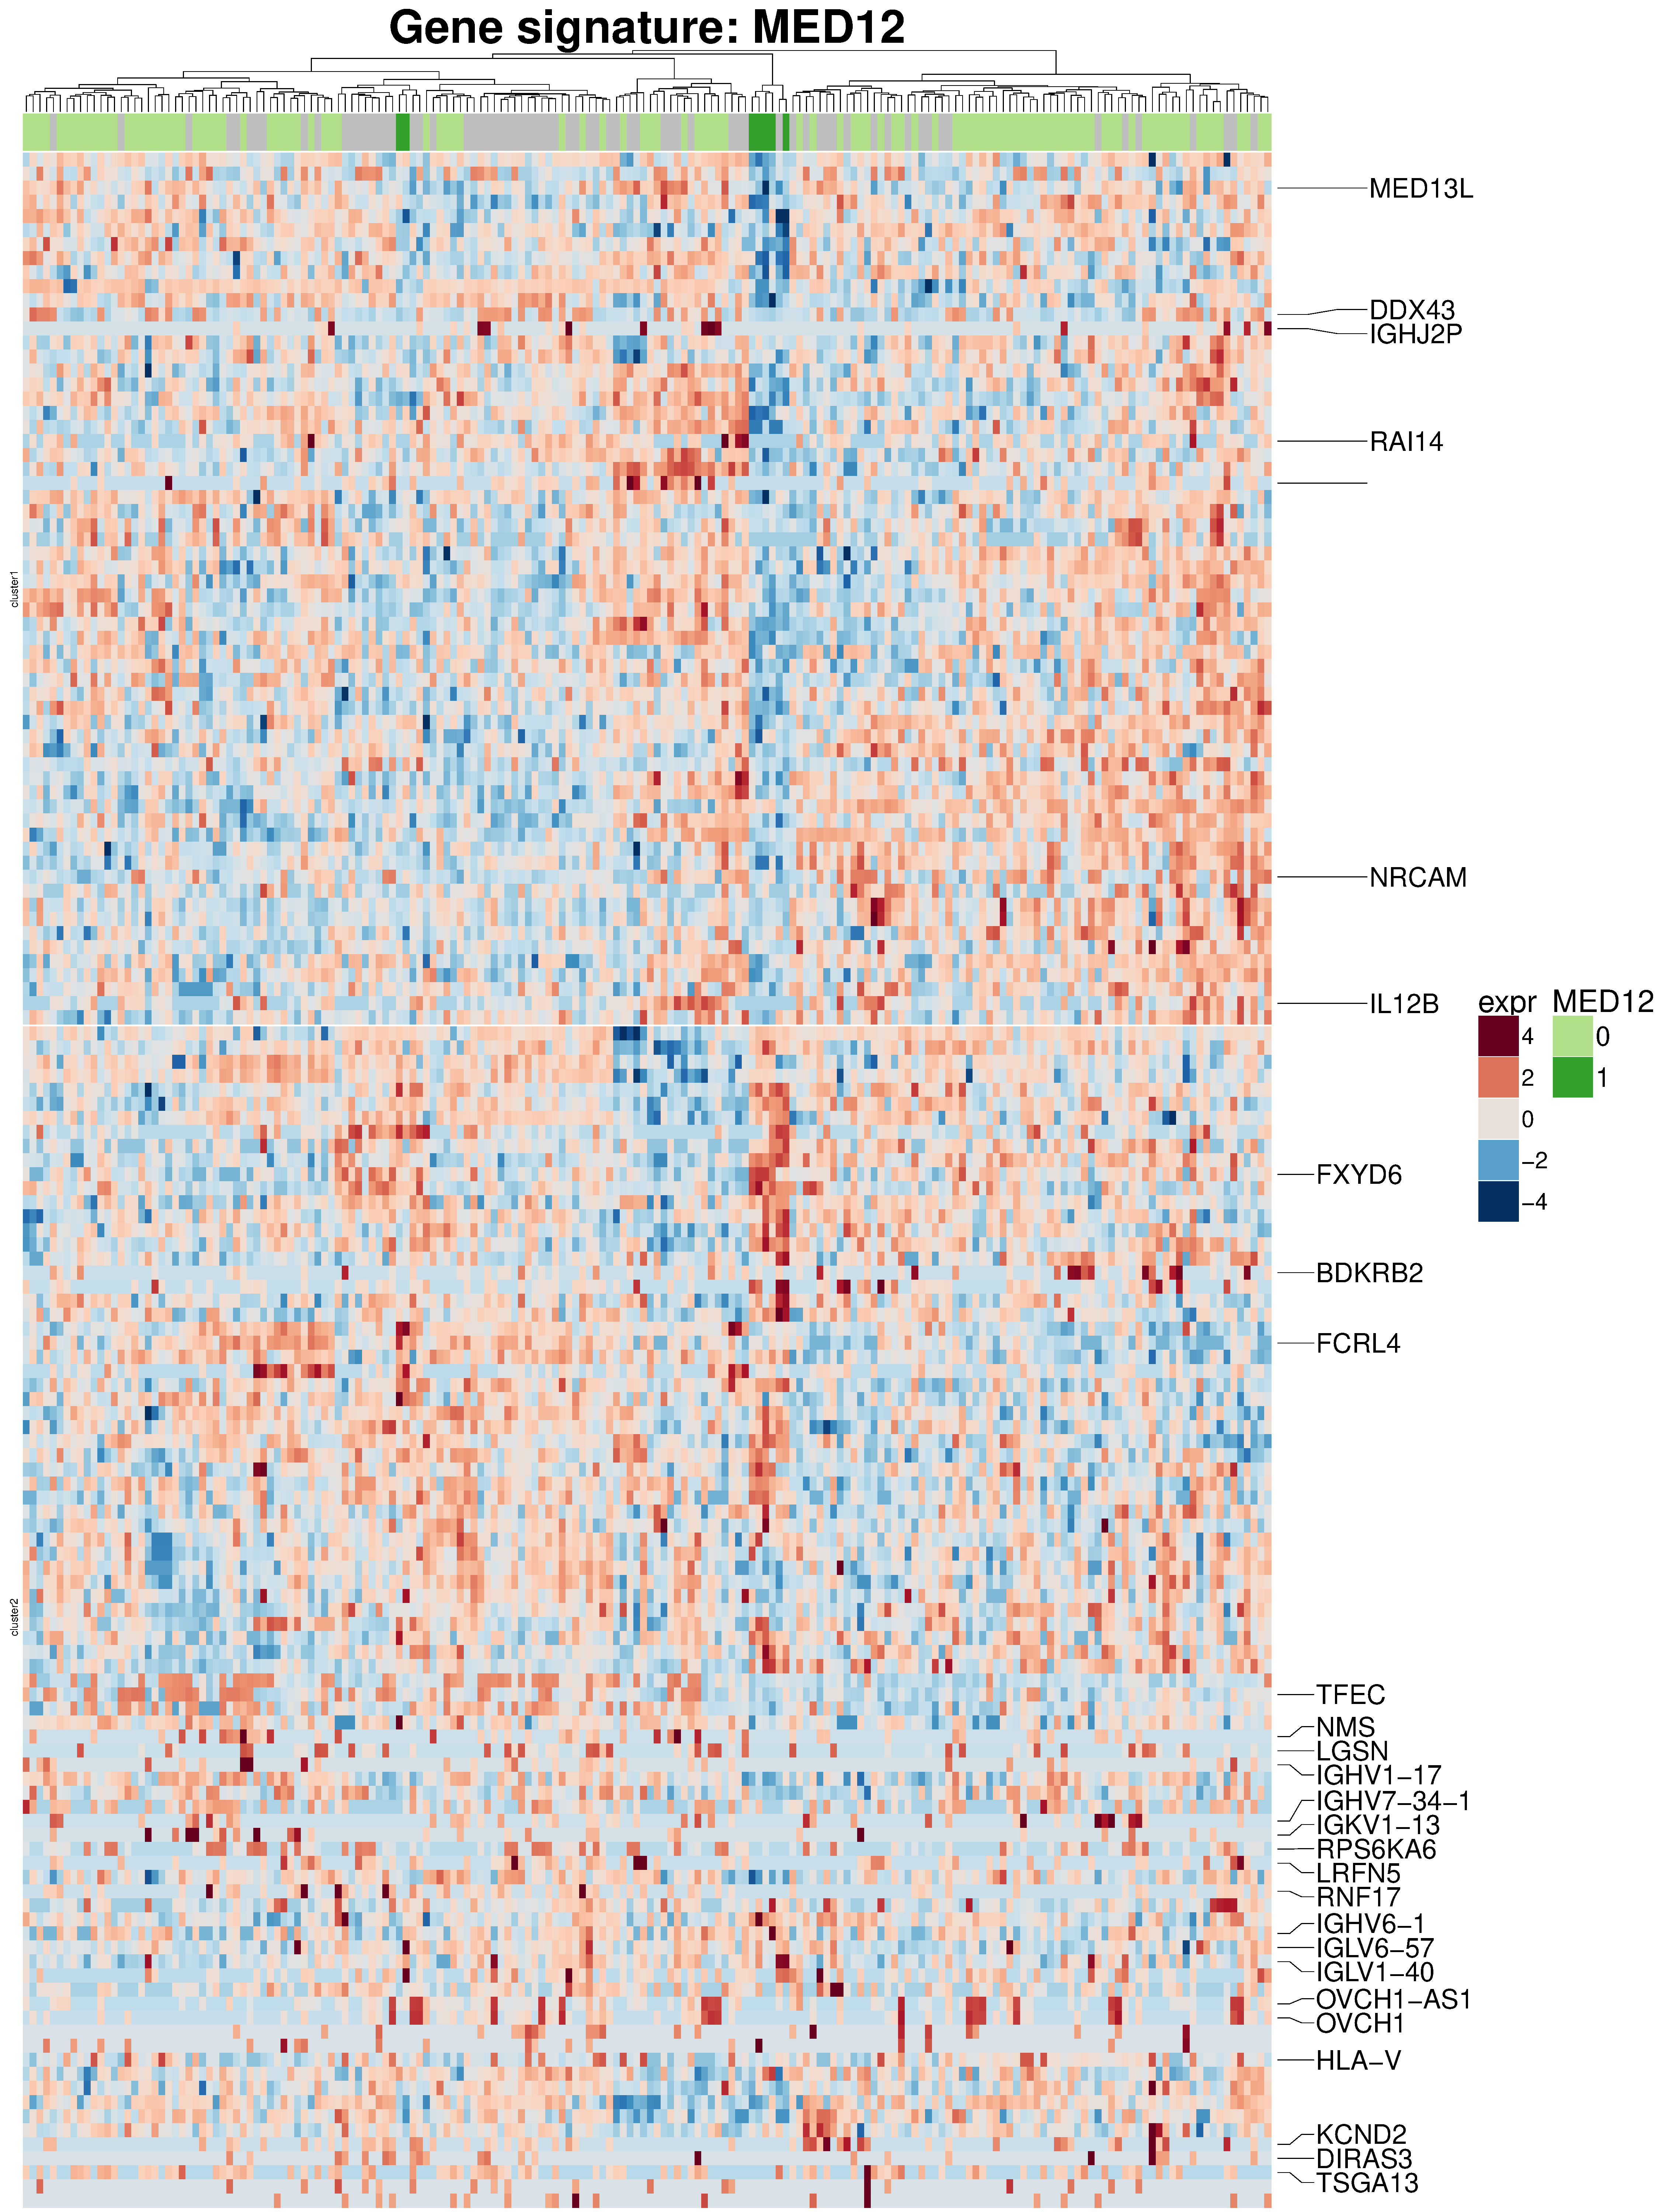
\includegraphics[width=0.5\textwidth]{/home/almut/Dokumente/git/Transcriptome_CLL/thesis/Figures/gene_exprMED12_gsea_Hallmark.pdf}
	\end{figure}
\end{frame}
%
%
\begin{frame}[c]
	\frametitle{Co-occurrence}
	\begin{figure}
		\centering
		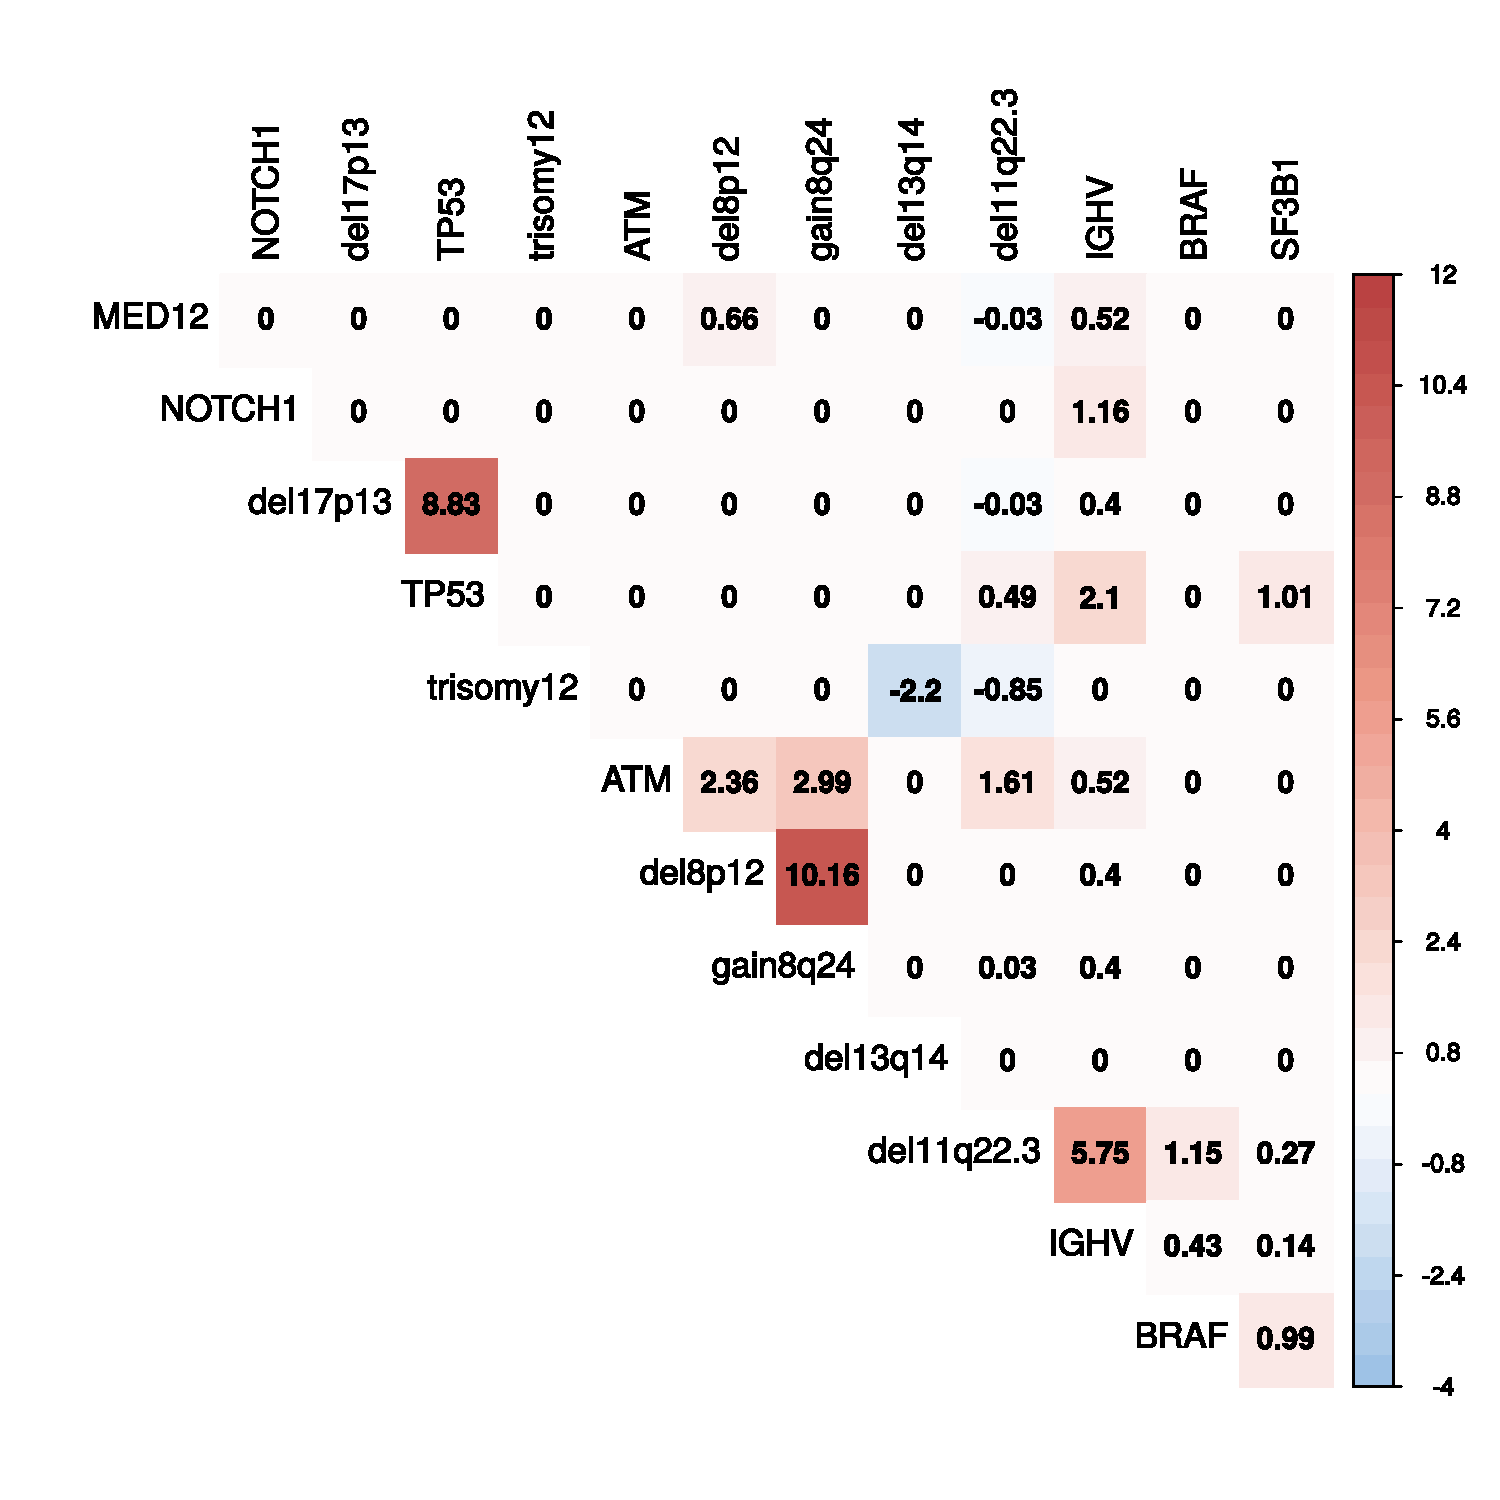
\includegraphics[width=0.55\textwidth]{/home/almut/Dokumente/git/Transcriptome_CLL/thesis/Figures/corplot_chiquare.pdf}
		\caption{-$\log_{10}$(pvalue) for co-occurrence of genetic variants calculated by $\chi^2$-square test. The sign indicates the direction of association.}
	\end{figure}
\end{frame}
%
%
\section{Conclusion}
%
%
\begin{frame}[c]
	\frametitle{Summary II}
	\begin{itemize}
		\item \textbf{IGHV} signature
		\begin{itemize}
			\item Differentially expressed genes are ernriched in B cell receptor signaling
			\item Marker genes ZAP70 and CD38 
		\end{itemize}
		\item \textbf{Trisomy12} signature
		\begin{itemize}
			\item Up regulation of integrins (ITGAM, ITGB2,...)
			\item CD49d
			\item Increased lymphnode homing?
		\end{itemize} 
		\item Differential gene expression pattern in 8 of 13 variants
		\item \textbf{Tumor epistatsis} (drug sensitivity, gene expression)
	\end{itemize}
\end{frame}
%  
%
\begin{frame}[c]
	\frametitle{Directions of epistatic interactions by Fischer et al.}
	\begin{figure}
		\centering
		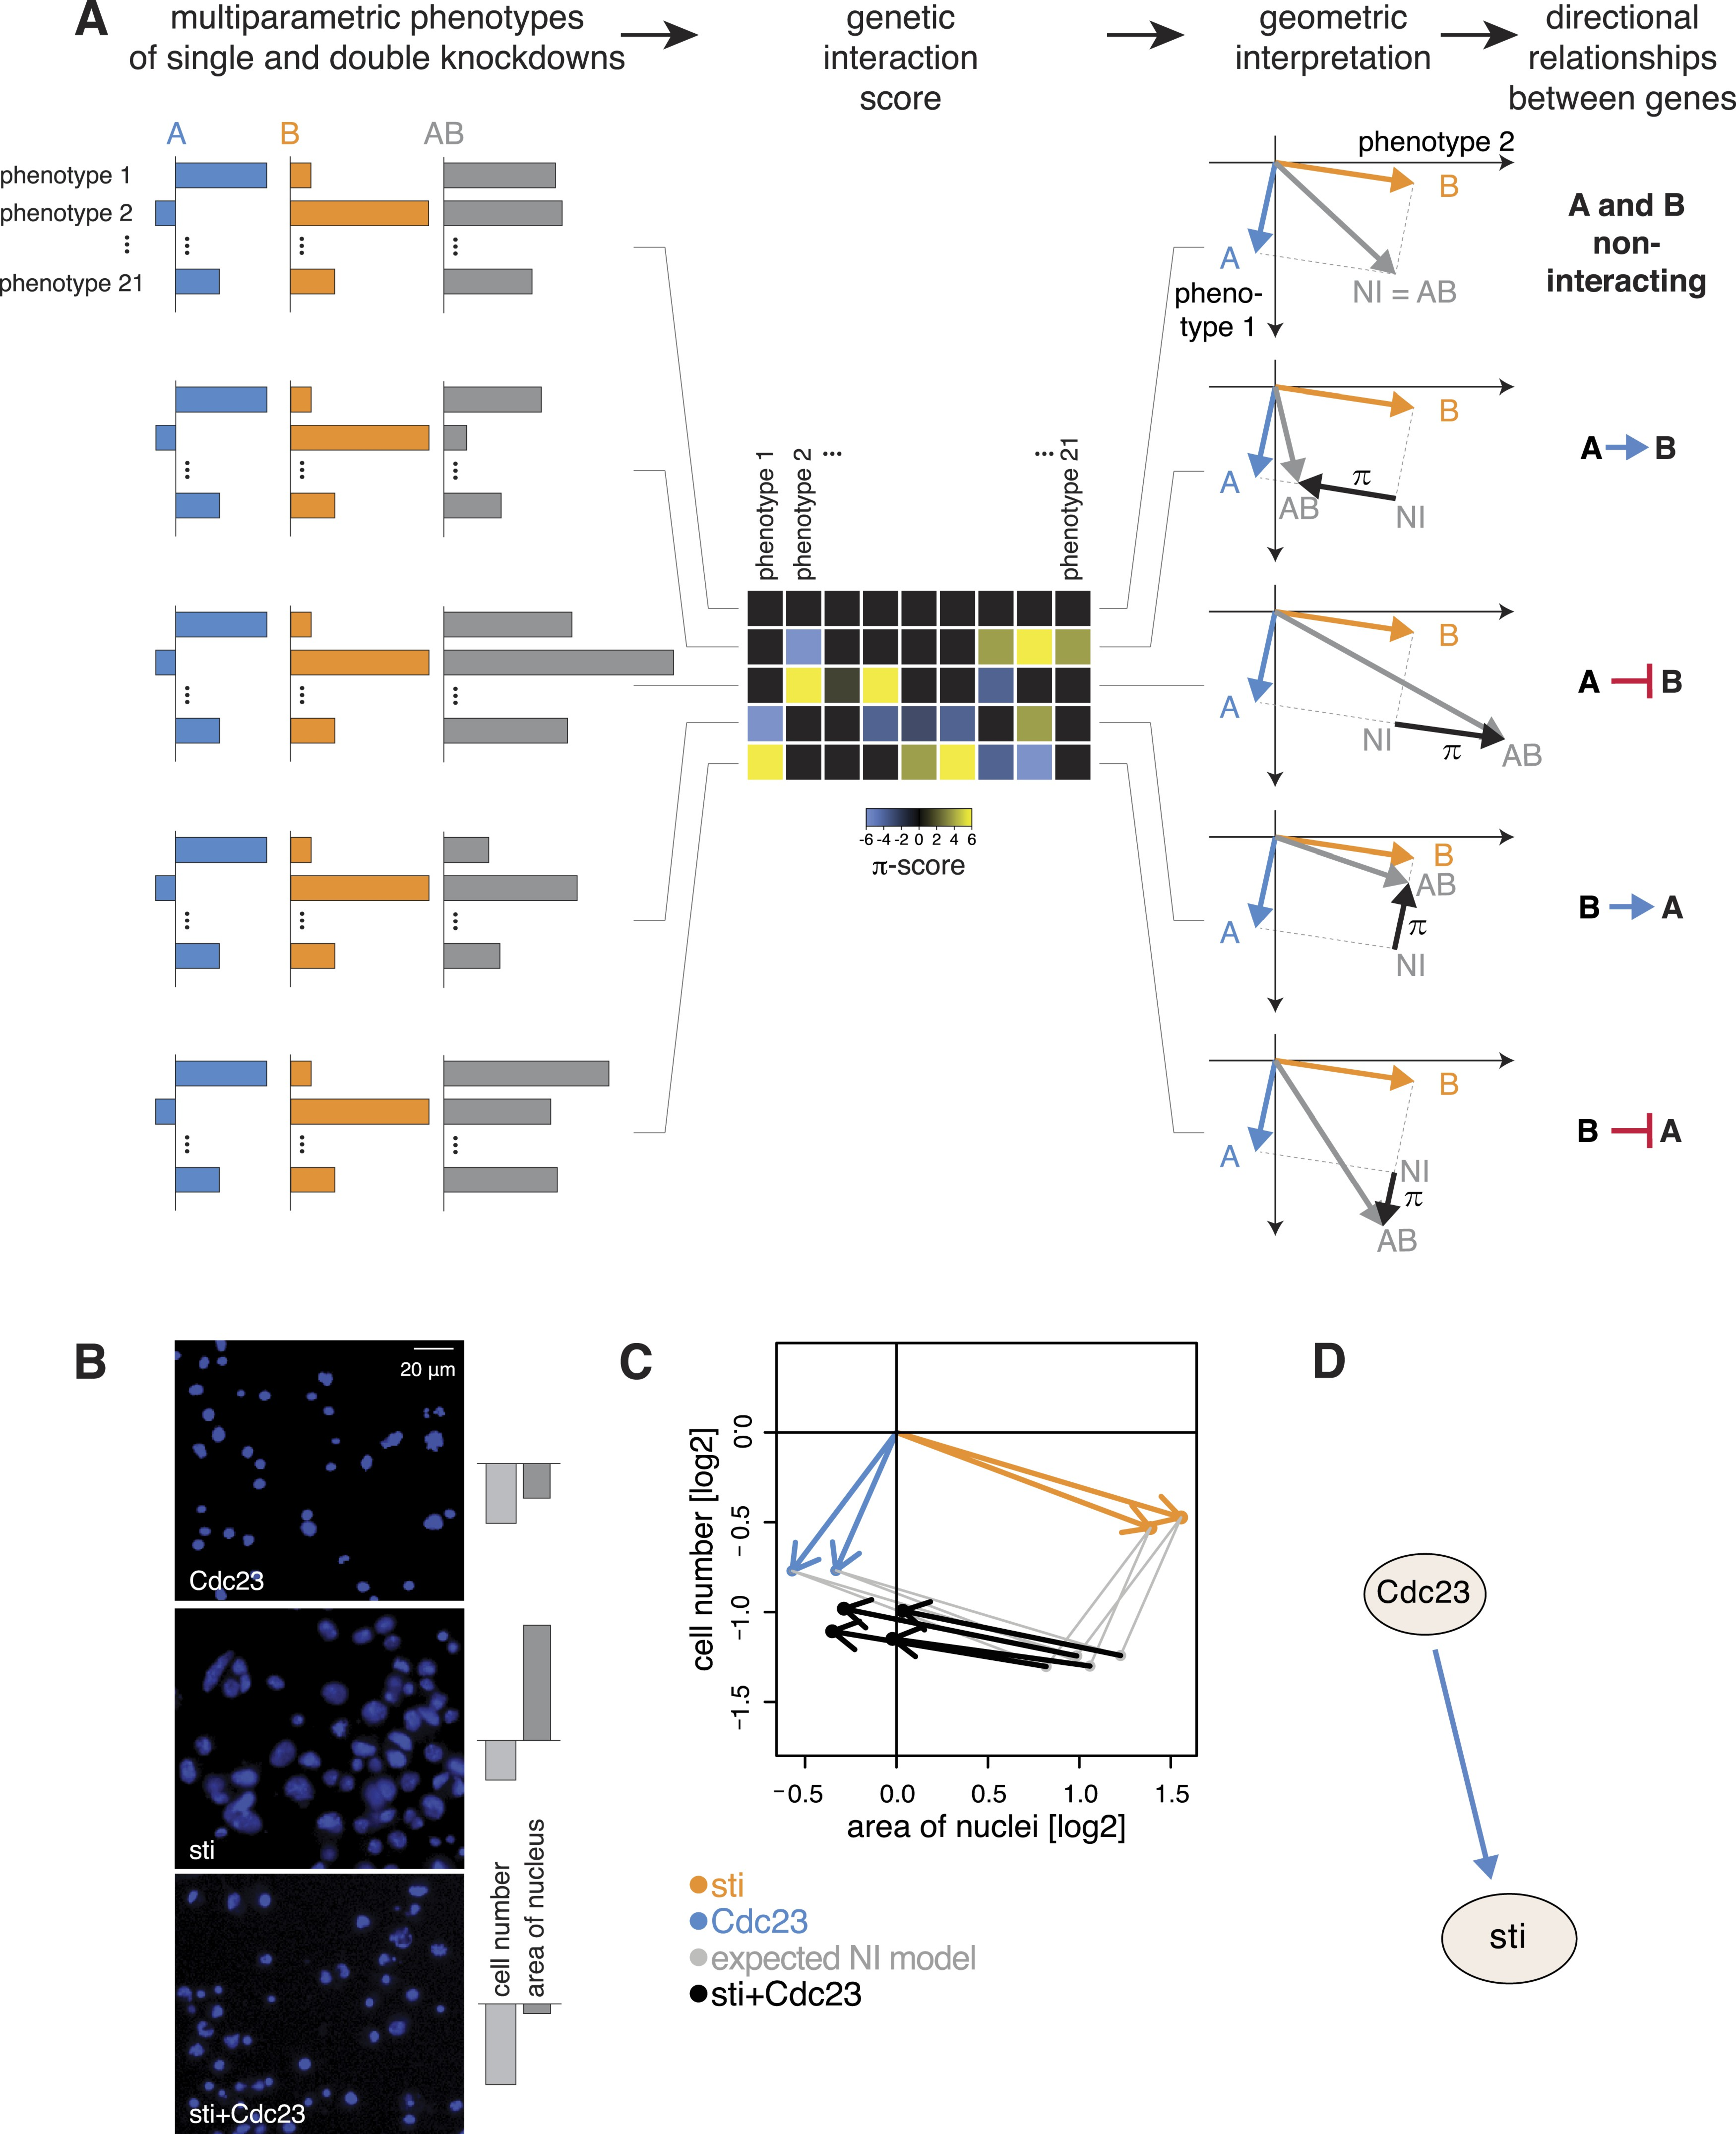
\includegraphics[width=0.5\textwidth]{/home/almut/Dokumente/git/Transcriptome_CLL/presentation/figures/Fischer_directions.pdf}
	\end{figure}
\end{frame}
%
%
\begin{frame}[c]
	\frametitle{Outlook}
	\begin{itemize}
		\item directions/mixed epistasis model? epiNEM
		\item role of TPL2 in Trisomy12 and IGHV-M
		\item lymphnode homing/integrins in Trisomy12
		\item enrichment tests 
	\end{itemize}
\end{frame}

\section{End}
\end{document}
